%%%%%%%%%%%%%%%%%%%%%%%%%%%%%%%%%%%%%%%%%%%%%%%%%%%%%%%%%%%%%%%%%%%%%%%

% Einbinden des Seiten Layouts
% Dokumentation des KOMA-Script-Packets: scrbook
%%%%%%%%%%%%%%%%%%%%%%%%%%%%%%%%%%%%%%%%%%%%%%%%%%%%%%%%%%%%%%%%%%%%%%%
%% Optionen zum Layout des Artikels                                  %%
%%%%%%%%%%%%%%%%%%%%%%%%%%%%%%%%%%%%%%%%%%%%%%%%%%%%%%%%%%%%%%%%%%%%%%%
\documentclass[            %% KOMA-Skript Dokumentklassen verwenden
draft = false,             		% Entwurfsmodus
paper = A4,                		% Papierart
% paper = landscape,       		% Seite im Querformat setzen
pagesize = pdftex,         		% Pagesize an pdfTeX anpassen
% pagesitze = xetex,       		% Pagesize an XeTeX anpassen
fontsize = 12pt,           		% Schriftgröße (12pt, 11pt (Standard))
%BCOR = 10mm,                	% Bindekorrektur
DIV=15,                    		% Satzspiegelfaktor, je größer, desto mehr Text auf Seite
twoside = false,           		% Doppelseiten (Ein|Aus|Semi)
twocolumn = false,         		% zweispaltiger Satz
parskip = full,           		% Absatzformatierung s. scrguide 3.1
%abstract = true,         		% Überschrift über Abstract an (nicht bei scrbook aktiv)
chapterprefix = false,      		% Layout der Kapitelüberschriften
appendixprefix = true,     		% Layout der Anhangüberschriften
headinclude = false,       		% Kopfzeile zu Text betrachten (für Satzspiegelberechnung)
footinclude = false,       		% Fußzeile zu Text betrachten (für Satzspiegelberechnung)
mpinclude = false,         		% Rand zum Text betrachten (für Satzspiegelberechnung)
% headlines = 1.25,        		% Anzahl der Kopfzeilen
% headheight = 2cm,        		% Höhe der Kopfzeile
% headsepline = true,      		% Trennline zum Seitenkopf
% footsepline = true,      		% Trennline zum Seitenfuß
numbers = auto,            		% KOMA-Skript setzt Endpunktierung im Inahltsverzeichnis.
cleardoublepage = plain,   		% Einstellung des Seitenstils für eingefügte Vakatseiten
% leqno,                   		% Nummerierung von Gleichungen links
% fleqn,                   		% Ausgabe von Gleichungen linksbündig
footnotes = multiple,      		% Mehrer aufeinander folgende Fußnoten durch Komma trennen
titlepage = true,          		% Titelei auf eigener Seite \maketitle[Seitenanzahl]
%headings = openright,     		% Kapitel auf rechter Seite beginnen, ggf. Vakatseiten
headings = normal,         		% Normalgroße Überschriften
open = right,              		% Seiten rechts beginnen
%toc = listof,
%toc = listof,              		% Abb.- und Tab.verzeichnis im Inhaltsverzeichnis
%toc = noindex,             		% Index im Inhaltsverzeichnis (index|noindex)
%toc = sectionentrywithoutdots,
%toc = chapterentrywithoutdots,
%bibliography = openstyle,  		% Offener Darstellungsstil der Bibliographie
listof = chaptergapline,   		% Abb.- und Tab.verzeichnis werden nach Kapitel geordnet
overfullrule = true,
numbers=noenddot                % keine Punkte in Kapitelnummern
]{scrbook}


% Einbinden eigener Kommandos
%%%%%%%%%%%%%%%%%%%%%%%%%%%%%%%%%%%%%%%%%%%%%%%%%%%%%%%%%%%%%%%%%%%%%%%
%% Spezielle Kommandos für die Bearbeitung des Projekts
% Fügt eine leere Seite ein
\newcommand*{\blankpage}{
   \clearpage{
      \pagestyle{empty}
      \cleardoublepage
   }
}

% Ändert die Schriftart
\newcommand*{\changefont}[3]{
\fontfamily{#1}  \fontseries{#2}  \fontshape{#3}  \selectfont}

% Verhalten der Gleichungs-Zähler
\newcommand*{\subeq}{\renewcommand\theequation{\theparentequation{}-\arabic{equation}}}

%%%%%%%%%%%%%%%%%%%%%%%%%%%%%%%%%%%%%%%%%%%%%%%%%%%%%%%%%%%%%%%%%%%%%%%
%% Kommandos zum Einfügen von Querverweisen
%% Deutsche Version

% Markiert eine indirekte Zitierung.
% #1: Seitennummer
% #2: Literaturreferenz
\newcommand*{\vgl}[2]{(vgl. \cite[S.~#2]{#1})}

% Markiert eine indirekte Zitierung mit 2 Verweisen
% #1: Seitennummer Verweis 1
% #2: Literaturreferenz 1
% #3: Seitennummer Verweis 2
% #4: Literaturreferenz 2
\newcommand*{\Vgl}[4]{(vgl. \cite[S.~#2]{#1} und \cite[S.~#4]{#3})}

% Deklariert eine Quelle.
% #1: Literaturreferenz
\newcommand*{\source}[1]{Quelle:~\cite{#1}}

% Verweist auf eine Quelle
% #1: Literaturreferenz
\newcommand*{\refSource}[1]{\cite{#1}}

% Verweist auf zwei Quellen
% #1: Literaturreferenz 1
% #2: Literaturreferenz 2
\newcommand*{\RefSource}[2]{\cite{#1, #2}}

% Fügt einen Verweis zu einem Bild ein.
% #1: Referenzname
\newcommand*{\refFig}[1]{\textbf{Abbildung~\ref{#1}}}

% Fügt einen Verweis zu einer Tabelle ein.
% #1: Referenzname
\newcommand*{\refTab}[1]{Tabelle~\ref{#1}}

% Fügt einen Verweis zu einem Kapitel ein.
% #1: Referenzname
\newcommand*{\refChpt}[1]{\textbf{Kapitel~\ref{#1}}}

% Fügt einen Verweis zu einem Abschnitt ein.
% #1: Referenzname
\newcommand*{\refSec}[1]{\textbf{Abschnitt~\ref{#1}}}
\newcommand*{\refAtt}[1]{\textbf{Anhang~\ref{#1}}}

% Fügt einen Verweis zu einem Unterabschnitt ein.
% #1: Referenzname
\newcommand*{\refSubSec}[1]{Unterabschnitt~\ref{#1}}

% Fügt einen Verweis zu einem Codeabschnitt ein.
% #1: Referenzname
\newcommand*{\refCode}[1]{Quellcode~\ref{#1}}

% Fügt einen Verweis zu einer Gleichung ein.
% #1: Referenzname
\newcommand*{\refEqu}[1]{Gleichung~\textnormal{(\ref{#1})}}

% Fügt ein kursiven Querverweis zu einem Bild ein.
% #1: Referenzname
\newcommand*{\seeFig}[1]{(s. \refFig{#1})}

% Fügt ein kursiven Querverweis zu einer Tabelle ein.
% #1: Referenzname
\newcommand*{\seeTab}[1]{(siehe \refTab{#1})}

% Fügt ein kursiven Querverweis zu einem Abschnitt ein.
% #1: Referenzname
\newcommand*{\seeSec}[1]{(s. \refSec{#1})}
\newcommand*{\seeAtt}[1]{(s. \refAtt{#1})}

% Fügt ein kursiven Querverweis zu einem Kapitel ein.
% #1: Referenzname
\newcommand*{\seeChpt}[1]{(siehe \refChpt{#1})}

% Fügt ein kursiven Querverweis zu einem Codeabschnitt ein.
% #1: Referenzname
\newcommand*{\seeCode}[1]{(siehe \refCode{#1})}

% Fügt ein kursiven Querverweis zu einer Gleichung ein.
% #1: Referenzname
\newcommand*{\seeEqu}[1]{(siehe \refEqu{#1})}

% Fügt ein kursiven Querverweis zu zwei Gleichungen ein.
% #1: Referenzname 1
% #2: Referenzname 2
\newcommand*{\SeeEqu}[2]{(siehe \refEqu{#1} und \refEqu{#2})}

\newcommand{\addtotoc}[1]{
\cleardoublepage
\phantomsection
\addcontentsline{toc}{chapter}{\textbf{#1}}
}

%%%%%%%%%%%%%%%%%%%%%%%%%%%%%%%%%%%%%%%%%%%%%%%%%%%%%%%%%%%%%%%%%%%%%%%
\makeatletter
\newcommand{\faculty}[1]{\gdef\@faculty{#1}}
\newcommand{\@faculty}{\@latex@warning@no@line{No \noexpand\faculty given}}
\newcommand{\thesisType}[1]{\gdef\@thesisType{#1}}
\newcommand{\@thesisType}{\@latex@warning@no@line{No \noexpand\thesisType given}}
\newcommand{\erstpruefer}[1]{\gdef\@erstpruefer{#1}}
\newcommand{\@erstpruefer}{\@latex@warning@no@line{No \noexpand\erstpruefer given}}
\newcommand{\zweitpruefer}[1]{\gdef\@zweitpruefer{#1}}
\newcommand{\@zweitpruefer}{\@latex@warning@no@line{No \noexpand\zweitpruefer given}}
\newcommand{\matrikelnummer}[1]{\gdef\@matrikelnummer{#1}}
\newcommand{\@matrikelnummer}{\@latex@warning@no@line{No \noexpand\matrikelnummer given}}

\renewcommand*{\maketitle}{
\begin{titlepage}
   \centering
   \vspace*{\fill}
   {\textbf{\Huge{\@title} \label{title}} \par}
   \vspace{1cm}
   {\LARGE \@subject \par}
   \vspace{2.3cm}
   {\LARGE{{\@thesisType} von \par \@author} \par}
   {\vspace{2.6cm}}
   {\LARGE{\@date}}
   \vfill
\end{titlepage}
}
\makeatother


% Einbinden der Packages
\pagestyle{empty}
% Deutsche Anpassungen %%%%%%%%%%%%%%%%%%%%%%%%%%%%%%%%%%%%%%%%%%%%%%%%%%%%%
\usepackage[T1]{fontenc}				% Schriftkodierung
\usepackage[utf8]{inputenc}				% Eingabekodierung

\usepackage[english,ngerman]{babel}		% Neue deutsche Rechtschreibung verwenden
\addto\captionsngerman{					% Name des Literaturverzeichnisses verändern
  \renewcommand{\bibname}{Quellenverzeichnis}
}
\usepackage{microtype}					% verbessert Umbruch von Texten
\usepackage{scrhack}

% URL %%%%%%%%%%%%%%%%%%%%%%%%%%%%%%%%%%%%%%%%%%%%%%%%%%%%%%%%%%%%%%%%%%%%%%
\usepackage{url}						% Links durch \url{}

\usepackage[
  left=3.8cm,
  right=2.8cm,
  top=3.5cm,
  bottom=3.5cm,
]{geometry}

\usepackage[normalem]{ulem}

\makeatletter
\let\oldTitle\title
\renewcommand{\title}[1]{
   \oldTitle{#1}
   \gdef\@utitle{\uline{#1}}
}
\newcommand{\@utitle}{\@latex@warning@no@line{No \noexpand\Title given}}
\newcommand{\underlinedtitle}{\@utitle}
\makeatother

\usepackage[sfdefault]{roboto}					% Roboto Schriftart
\usepackage[section]{placeins}

\usepackage[                  % Package für Farbe
   pdftex,                    % Ausgabe für pdfTeX
   %xetex,                    % Ausgabe für XeTeX
   hyperref,                  % Hyperref-Support
   svgnames,                             % Zusätzliche Farben per Name hinzufügen
   x11names,                             % un nochmehr Farben
   showerror                  % Fehlermeldung bei Verwendung undefinierter Farbe
   ]{xcolor}%

\definecolor{dkgreen}{rgb}{0,0.6,0}
\definecolor{mauve}{rgb}{0.58,0,0.82}

%% Packages für Grafiken & Abbildungen %%%%%%%%%%%%%%%%%%%%%%%%%%%%%%%%%%%%%%
\usepackage[pdftex]{graphicx}			% Zum Laden von Grafiken
   \graphicspath{{Bilder/}}				% Standardpfad für Bilder/Grafiken

\usepackage{fancybox}		% Ermöglicht zeichnen von Boxen von definierter Länge


% fancy cross-referencing \fref & \Fref
\usepackage[german, plain]{fancyref}


\usepackage[                  % Bildunterschriften
   format = hang,             % Ausrichtung
%   indention = 0.5cm,        % Texteinzug ab 2. Zeile
   labelformat = default,     % Bezeichnerformatierung
   labelsep = colon,          % Bezeichner-Trennzeichen
%  textformat = period,       % Textformatierung (Textendzeichen)
   justification = justified, % Text als Blocksatz setzen
   singlelinecheck = true,    % 1-Zeilen-Beschriftungen --> zentrieren erlaubt
   font = {it, small},        % Beschriftungsformat
   labelfont = bf,			  % Bezeichnerformat (Bild x.y...)
%   textfont = it,            % Textformat
   margin = 0pt,              % Beschriftungsrand (auch links/rechts möglich {0pt, 0pt})
   oneside,                   % Einseitiger Textsatz
%   twoside,                  % Zweiseitiger Textsatz
   parskip = 5pt,             % Abstand zwischen Absätzen in Beschriftungen
   skip = 8pt,                % Abstand von Beschriftung
   listfigurename = Bilderverzeichnis,	% Abbildungen anstatt Abbildungsverzeichniss
   listtablename  = Tabellen,           % Tabellen anstatt Tabellenverzeichnis
   figurewithin = chapter,    % Zählerbegrenzung festlegen (also Bild 3.1 anstatt Bild 43)
   tablewithin = chapter      % Zahlerbegrenzung festlegen
   ]{caption}

% Tabellen %%%%%%%%%%%%%%%%%%%%%%%%%%%%%%%%%%%%%%%%%%%%%%%%%%%%%%%%%%%%%%%%%%%%%%%%%
\usepackage{array}             % Standarderweiterung für Tabellen
\usepackage{diagbox}		   % Diagonale linie durch Zelle

% Bibliographiestil %%%%%%%%%%%%%%%%%%%%%%%%%%%%%%%%%%%%%%%%%%%%%%%%%%%%%%%%%%%%%%%%
%\usepackage[				% Erweiterung der Basisfunktionalität
%	numbers,				% Nummern
%	square,					% Eckige Klammern
%    sort&compress,			% Multiple Zitate sortieren und zusammenfassen
%    longnamesfirst			% Erstes Zitat mit vollen Namen
%   ]
%   {natbib}

%{Bibliographie/ka-style}
%   \setcitestyle{
%     authoryear,% Author-Year-Style
%      square,   % Eckige Klammern
%     semicolon, % semicolon als Trennzeichen
%      aysep{},% Kein explizites Trennzeichen zwischen Author und Year
%      yysep{;}% Komma als Trennzeichen zwischen mehreren Jahren
%      }

% Listings %%
\usepackage{listings}
\usepackage{lipsum}

% Spaltendefinition rechtsbndig mit definierter Breite
%\newcolumntype{w}[1]{>{\raggedleft\hspace{0pt}}p{#1}}

%% Mathematik-Packages%%%%%%%%%%%%%%%%%%%%%%%%%%%%%%%%%%%%%%%%%%%%%%%%%
\usepackage{amsmath}             % AMS Mathematikumgebungen/-erweiterungen
\usepackage{amssymb}             % AMS Symbol/Font-Paket
%\usepackage{accents}            % Erweiterung für Akzente im Mathematik-Modus
\usepackage{mathcomp}            % Symbolerweiterungen für Mathematikmodus
%\usepackage{cancel}             % Durchstreicehn in Mathematikumgebung

% Title format Anpassen
\makeatletter
\renewcommand{\chapterlinesformat}[3]{\@hangfrom{\bfseries{#2}}\mdseries{#3}}
\renewcommand{\sectionlinesformat}[4]{\@hangfrom{\hskip#2\bfseries{#3}}{\mdseries{#4}}}
\makeatother

% TODO: handle more than only chapter and section

\usepackage[                  % Paket zum Navigieren innerhalb eines Dokuments
   plainpages=true,           % Arabische Zeichen für Link-Darstellung
   bookmarksopen=true,        % Lesezeichenbaum aufklappen
   bookmarksopenlevel=1,      % Aufklapptiefe
   pdfborder={0 0 0},         % Rahmenfarbe
   pdfpagemode=UseOutlines,	% Ansicht im Adobe Reader
   pdftex,                    % Ausgabe mit pdfTeX
   pdfusetitle
   ]{hyperref}
   \hypersetup{
   pdfborder={0 0 0},			% Kein Rand um Links
	plainpages=false,			% Zur korrekten Erstellung der Bookmarks
	hypertexnames=false			% Zur korrekten Erstellung der Bookmarks
   }


\usepackage[
   printonlyused
   ]{acronym}

\usepackage{upgreek}

\lstset{ %
    basicstyle=\footnotesize\ttfamily,	% the size of the fonts that are used for the code
    numbers=left,						% where to put the line-numbers
    numbersep=5pt,						% how far the line-numbers are from the code
    backgroundcolor=\color{white},      % choose the background color. You must add \usepackage{color}
    showspaces=false,               % show spaces adding particular underscores
    showstringspaces=false,         % underline spaces within strings
    showtabs=false,                 % show tabs within strings adding particular underscores
    rulecolor=\color{black},        % if not set, the frame-color may be changed on line-breaks within not-black text (e.g. commens (green here))
    tabsize=2,                      % sets default tabsize to 2 spaces
    captionpos=t,                   % sets the caption-position to bottom
    breaklines=true,                % sets automatic line breaking
    breakatwhitespace=false,        % sets if automatic breaks should only happen at whitespace
    title=\lstname,                 % show the filename of files included with \lstinputlisting;
									% also try caption instead of title
    keywordstyle=\color{blue},      % keyword style
    commentstyle=\color{dkgreen},   % comment style
    escapeinside={\%*}{*)},         % if you want to add LaTeX within your code
    morekeywords={*,...}            % if you want to add more keywords to the set
    frame=b,
    stringstyle=\color{mauve}\ttfamily,	% Farbe der String
    showspaces=false,					% Leerzeichen anzeigen ?
    showtabs=false,						% Tabs anzeigen ?
    xleftmargin=17pt,
    framexleftmargin=17pt,
    framexrightmargin=5pt,
    framexbottommargin=4pt,
    showstringspaces=false      % Leerzeichen in Strings anzeigen ?
}

\DeclareCaptionFont{white}{\color{white}}
\DeclareCaptionFormat{listing}{\colorbox[cmyk]{0.43, 0.35, 0.35,0.01}{\parbox{\textwidth}{\hspace{15pt}#1#2#3}}}
%\captionsetup[lstlisting]{format=listing,labelfont=white,textfont=white, singlelinecheck=false, margin=0pt, font={bf,footnotesize}}

\usepackage{tabularx}
\usepackage{booktabs}
\usepackage{caption}
\usepackage{csquotes}
\usepackage{helvet}
\usepackage{mathpazo}
\usepackage[binary-units=true]{siunitx}
\usepackage{subcaption}
\usepackage{enumitem}
\setlist[description]{style=nextline}
\usepackage{romannum}

\renewcaptionname{ngerman}\figureautorefname{Abb.}

\tolerance 1414
\hbadness 1414
\emergencystretch 1.5em
\hfuzz 0.3pt
\widowpenalty=10000
\vfuzz \hfuzz
\raggedbottom

% XXX: ugly
%\makeatletter
%  \let\ps@plain\ps@empty
%\makeatother

\DeclareTOCStyleEntries[linefill=\hfill]{tocline}{section,subsection,subsubsection,figure,table}
\DeclareTOCEntryStyle{section}{section}
\addtokomafont{chapterentry}{\mdseries}
\addtokomafont{chapterentrypagenumber}{\bfseries}
\newcommand*{\SavedOriginaladdchaptertocentry}{}
\let\SavedOriginaladdchaptertocentry\addchaptertocentry

\setuptoc{toc}{indent}
\RedeclareSectionCommand[tocpagenumberformat=\bfseries]{section}%
\RedeclareSectionCommand[tocpagenumberformat=\bfseries]{subsection}%

\renewcommand*{\addchaptertocentry}[2]{%
   \SavedOriginaladdchaptertocentry{\bfseries{#1}}{
       \texorpdfstring{\textbf{#2}}{#2}}
}

\newcommand*{\SavedOriginaladdsectiontocentry}{}
\let\SavedOriginaladdsectiontocentry\addsectiontocentry
\renewcommand*{\addsectiontocentry}[2]{%
   \SavedOriginaladdsectiontocentry{\bfseries{#1}}{#2}
}

\newcommand*{\SavedOriginaladdsubsectiontocentry}{}
\let\SavedOriginaladdsubsectiontocentry\addsubsectiontocentry
\renewcommand*{\addsubsectiontocentry}[2]{%
   \SavedOriginaladdsubsectiontocentry{\bfseries{#1}}{#2}
}

\makeatletter
%\renewcommand\frontmatter{%
%   \cleardoublepage
%   \@mainmatterfalse
%   \pagenumbering{Roman}}
%\makeatother
\DeclareNewTOC[
   name=Formel,
   listname={Formelverzeichnis}
]{equation}
\setuptoc{equation}{chapterlist}

\newcommand{\myequations}[1]{%
\addcontentsline{equation}{chapter}{\protect\numberline{\theequation}#1}}


% Einbinden eigener Makros
\newcommand*{\maintoc}{% Hauptinhaltsverzeichnis
  \begingroup
    \@fileswfalse% kein neues Verzeichnis öffnen
    \renewcommand*{\appendixattoc}{% Trennanweisung im Inhaltsverzeichnis
      \value{tocdepth}=-10000 % lokal tocdepth auf sehr kleinen Wert setzen
    }%
    \tableofcontents% Verzeichnis ausgeben
  \endgroup
}
\newcommand*{\appendixtoc}{% Anhangsinhaltsverzeichnis
  \begingroup
    \edef\@alltocdepth{\the\value{tocdepth}}% tocdepth merken
    \setcounter{tocdepth}{-10000}% Keine Verzeichniseinträge
    \renewcommand*{\contentsname}{% Verzeichnisname ändern
      Anhang}%
    \renewcommand*{\appendixattoc}{% Trennanweisung im Inhaltsverzeichnis
      \setcounter{tocdepth}{\@alltocdepth}% tocdepth wiederherstellen
    }%
    \tableofcontents% Verzeichnis ausgeben
    \setcounter{tocdepth}{\@alltocdepth}% tocdepth wiederherstellen
  \endgroup
}
\newcommand*{\appendixattoc}{% Trennanweisung im Inhaltsverzeichnis
}
\g@addto@macro\appendix{% \appendix erweitern
  \if@openright\cleardoublepage\else\clearpage\fi% Neue Seite
  \phantomsection
  \addcontentsline{toc}{chapter}{\textbf{\appendixname}}% Eintrag ins Hauptverzeichnis
  \addtocontents{toc}{\protect\appendixattoc}% Trennanweisung in die toc-Datei
}

\g@addto@macro\appendix{%
  %\pagenumbering{Roman}%
  \addtocontents{toc}{\protect\renewcommand*{\protect\@pnumwidth}{3.5em}}%Seitenzahlen im Anhangverzeichnis nicht über Seitenrand hinaus. Problem entstand durch die langen römischen Zahlen. Siehe auch: http://www.komascript.de/node/608
}

% Kapitel Punkt entfernen
%\renewcommand{\autodot}{}

% Einbinen eigner Pakete
% Hie die eigenen benötigten Pakete einflegen
\usepackage[backend=biber, style=ieee, citestyle=ieee, dashed=false]{biblatex}

   % Einbinden des Literaturverzeichnisses
   \addbibresource{Literatur/Literatur_David.bib}
   \addbibresource{Literatur/Literatur_Dennis.bib}

% fix nodate
\xpatchbibdriver{online}
   {\printtext[parens]{\usebibmacro{date}}}
   {\iffieldundef{year}
     {. (o. D.). }
     {\printtext[parens]{\usebibmacro{date}}}}
   {}
   {\typeout{There was an error patching biblatex-ieee (specifically, ieee.bbx's @online driver)}}

\usepackage{tensor} % Formeln

\usepackage{fixfoot}
\DeclareFixedFootnote{\ver}{verfasst von Steinbeck \cite{steinbeck_entwicklung_2022}}
\DeclareFixedFootnote{\aus}{ausführlich behandelt in \cite[Steinbeck, Abschnitt~3.4]{steinbeck_entwicklung_2022}}
\DeclareFixedFootnote{\beh}{ausführlich behandelt in \cite[Steinbeck, Abschnitt~4.2]{steinbeck_entwicklung_2022}}
\usepackage{dirtree}

%Daten die Automatisch Verwendet werden
\author{David Gries}
\title{\texorpdfstring{\hspace{-0.3cm}
\includegraphics[width=6cm]{Bilder/thab_logo.png}\\[3cm]}{}Entwicklung einer KI-basierten Robotersteuerung mit Industrial ROS}
\subject{Automatische Erkennung und Lokalisierung von Objekten durch ein 3D-Kamerasystem}
\thesisType{Bachelorarbeit}
\faculty{Fakultät Ingenieurswissenschaften}
\erstpruefer{Prof. Dr. Hartmut Bruhm}
\matrikelnummer{2217395}

%%%%%%%%%%%%%%%%%%%%%%%%%%%%%%%%%%%%%%%%%%%%%%%%%%%%%%%%%%%%%%%%%%%%%%%
%%%                          Dokumentanfang                         %%%
%%%%%%%%%%%%%%%%%%%%%%%%%%%%%%%%%%%%%%%%%%%%%%%%%%%%%%%%%%%%%%%%%%%%%%%

\begin{document}
   % Dokument erstmalig initialisieren (Front Matter)
   \frontmatter
   \pagenumbering{Roman}
   % Deckblatt
   % Erste Titelseite
\newgeometry{margin=2cm}
\maketitle
\newgeometry{left=3.8cm, right=2.8cm, top=3.5cm, bottom=3.5cm}
% Zweite Titelseite
\newpage
\thispagestyle{empty}
\begin{center}
\makeatletter
\textbf{Entwicklung einer KI-basierten Robotersteuerung mit Industrial ROS}
Automatische Erkennung und Lokalisierung von Objekten durch ein 3D-Kamerasystem
\makeatother
\end{center}
\begin{flushleft}
   \vspace{10em}
   \textbf{Autor:}\\
   \makeatletter
   \@author\\
   \@matrikelnummer\\
   \makeatother
   \vspace{5em}
   \textbf{Prüfer:}\\
   \makeatletter
   \@erstpruefer\\
   \makeatother
   \vspace{10em}
   \begin{minipage}[b]{0.4\textwidth}
       
\includegraphics[scale=0.15]{Bilder/thab_logo.png}
   \end{minipage}
   \par
   \large{\MakeUppercase{\textbf{Technische Hochschule Aschaffenburg}}} \par
   \makeatletter
   \large{\MakeUppercase{\textbf{\@faculty}}} \par
   \makeatother
   \large{\MakeUppercase{\textbf{Würzburger Straße 45}}} \par
   \large{\MakeUppercase{\textbf{D-63743 Aschaffenburg}}} \par
    \vfill
\end{flushleft}

%%%%%%%%%%%%%%%%%%%%%%%%%%%%%%%%%%%%%%%%%%%%%%%%%%%%%%%%%%%%%%

\newpage
\thispagestyle{empty}
   \textbf{Erklärung zur Abschlussarbeit}

   Hiermit versichere ich, dass ich die vorliegende Arbeit selbständig verfasst
   und keine anderen Hilfsmittel als die angegebenen verwendet habe.
   Die Stellen, die anderen Werken
   (gilt ebenso für Werke aus elektronischen Datenbanken oder aus dem Internet)
   wörtlich oder sinngemäß entnommen sind, habe ich unter Angabe der Quelle
   und Einhaltung der Regeln wissenschaftlichen Zitierens kenntlich gemacht.
   Diese Versicherung umfasst auch in der Arbeit verwendete bildliche Darstellungen,
   Tabellen, Kartenskizzen und gelieferte Zeichnungen.

   Mir ist bewusst, dass Täuschungen nach der für mich gültigen Studien- und
   Prüfungsordnung / nach § 6 RaPO / § 48 BayVwVfG geahndet werden.

   Die Zustimmung zur elektronischen Plagiatsprüfung wird erteilt.
   \vspace{1.5cm}

   \begin{tabular}{@{}p{3.5cm}p{7cm}@{}}
    \hrulefill & \hrulefill \\
    Ort, Datum & Unterschrift des Verfassers / der Verfasserin \\
   \end{tabular}

   \vspace{1cm}
   \textbf{Veröffentlichung der Arbeit in der Bibliothek der Technischen Hochschule Aschaffenburg}

   Der Veröffentlichung der Master-/Bachelorarbeit in der Bibliothek
   der Technischen Hochschule Aschaffenburg wird zugestimmt.
   \vspace{1.5cm}

   \begin{tabular}{@{}p{3.5cm}p{7cm}@{}}
    \hrulefill & \hrulefill \\
    Ort, Datum & Unterschrift des Verfassers / der Verfasserin \\
   \end{tabular}

%%%%%%%%%%%%%%%%%%%%%%%%%%%%%%%%%%%%%%%%%%%%%%%%%%%%%%%%%%%%%%%%%%%

   %\chapter*{Abstract}
\newpage
\begin{center}
    \Large
    \textbf{Entwicklung einer KI-basierten Robotersteuerung mit Industrial ROS}
       
    \large
    Automatische Erkennung und Lokalisierung von Objekten durch ein 3D-Kamerasystem
        
    \vspace{0.4cm}
    \textbf{David Gries}
       
    \vspace{2cm}
    \textbf{Abstract}
\end{center}

Die vorliegende Arbeit befasst sich mit der Entwicklung einer KI-basierten Robotersteuerung auf Basis von ROS, die mithilfe eines 3D-Kamerasystems die Position und Art von Objekten erkennt. Diese nutzt das Intel RealSense 435 3D-Kamerasystem und den Objekterkennungsalgorithmus YOLOv3. Die Umsetzung des Systems erfolgt am 6-Achs-Knickarmroboter RV6L der Firma Reis Robotics. Es wird ein ROS-Paket implementiert, das die zweidimensionale Objektposition mit dem 3D-Bild der RealSense abgleicht, um zusätzlich zum Objektmittelpunkt dessen Abstand zur Kamera zu ermitteln. Der YOLOv3-Algorithmus weist eine geringe Fehlerrate bei der Klassifizierung auf und erkennt die Positionen der Objekte zuverlässig, kann jedoch nicht deren Orientierung feststellen. Im Vergleich zu traditioneller Computer Vision bietet der verwendete Deep Learning Algorithmus vor allem in Bezug auf den Einlernprozess und der möglichen Weiterentwicklung Vorteile.\\

This thesis describes the development of an AI-based robot controller using ROS. It uses a 3D camera system to recognize the position and class of unordered objects. To accomplish this, an Intel RealSense 435 3D camera system and the object recognition algorithm YOLOv3 are used. The system is implemented on the six-axis articulated arm robot RV6L from Reis Robotics. A ROS package that matches the two-dimensional object position with the three-dimensional image of the RealSense is implemented to determine the distance between the camera and the object center. The YOLOv3 algorithm has a low error rate in classification and reliably detects the positions of the objects, but cannot determine their orientation. Compared to traditional computer vision, the Deep Learning algorithm offers advantages especially in terms of the learning process and possible further development.

   \setcounter{page}{0}
   % Inhaltsverzeichnis einfügen
   \pagestyle{plain}
   \setcounter{secnumdepth}{3}                        % Tiefe des Inhaltsverzeichnisses festlegen
   \setcounter{tocdepth}{2}
   \maintoc                                           % Inhaltsverzeichnis erzeugen

   %%%%%%%%%%%%%%%%%%%%%%%%%%%%%%%%%%%%%%%%%%%%%%%%%%%%%%%%%%%%%%

   \newpage \phantomsection
   \addtotoc{Abkürzungsverzeichnis}
   %%%%%%%%%%%%%%%%%%%%%%%%%%%%%%%%%%%%%%%%%%%%%%%%%%%%%%%%%%%%%%
\chapter*{Abkürzungsverzeichnis}

\begin{acronym}[Abkuerzungen]
   % Numerische Abkürzungen

   % 'A'
   \acro{ANN}{Artificial Neural Network}
   % 'B'
   \acro{Bash}{Bourne-again Shell}
   % 'C'
   \acro{CMOS}{Complementary Metal-Oxide-Semiconductor}
   \acro{CNN}{Convolutional Neural Network}
   \acro{CP}{Continuous Path}
   \acro{CUDA}{Compute Unified Device Architecture}
   \acro{CV}{Computer Vision}
   % 'D'
   \acro{DCNN}{Deep Convolutional Neural Network}
   \acro{DL}{Deep Learning}
   % 'E'

   % 'F'

   % 'G'

   % 'H'
   \acro{HBBs}{Horizontal Bounding Boxes}
   % 'I'
   \acro{IoU}{Intersection over Union}
   % 'J'
 
   % 'K'

   % 'L'
   \acro{LTS}{Long Term Support}
   % 'M'

   % 'N'
   \acro{NMS}{Non Maximum Suppression}
   % 'O'
   \acro{OBBs}{Orientation Bounding Boxes}
   % 'P'
   \acro{PTP}{Point to Point}
   % 'Q'

   % 'R'
   \acro{ROS}{Robot Operating System}
   \acro{RNN}{Recurrent Neural Network}
   % 'S'
   \acro{SDK}{Software Development Kit}
   \acro{SIFT}{Scale-invariant Feature Transform}
   \acro{SoC}{System on a Chip}
   \acro{SURF}{Speeded up Robust Features}
   \acro{SVM}{Support Vector Machine}
   % 'T'
   \acro{TCP}{Tool Center Point}
   \acro{ToF}{Time of Flight}
   % 'U'

   % 'V'
   \acro{VM}{virtuelle Maschine}
   % 'W'

   % 'X'
   
   % 'Y'
   \acro{YOLO}{You Only Look Once}
   % 'Z'

\end{acronym}

   
   %%%%%%%%%%%%%%%%%%%%%%%%%%%%%%%%%%%%%%%%%%%%%%%%%%%%%%%%%%%%%%

   % Dokument initialisieren
   \mainmatter
   \pagestyle{headings}

   % Kapitel einbinden
   \chapter{Einleitung}

Roboter spielen aufgrund der schnellen Anpassungsmöglichkeit bei Produktionsprozessen, die heute einen hohen Stellenwert hat, eine immer wichtigere Rolle in der Industrie. Mit steigender Rechenleistung und dem schnellen Fortschritt im Bereich der Bilderkennung, vor allem unter Anwendung von \textit{\acp{CNN}}, findet die Erkennung von Objekten mit Kamerasystemen in immer mehr Bereichen der Robotik Anwendung. So können beispielsweise schon heute auf \textit{\ac{DL}} basierende Techniken, die noch vor Kurzem nur selten für einen praktischen Einsatz geeignet waren, Anwendung in der Industrie finden. Zukünftig kann \textit{\ac{DL}} für die Vereinfachung der Bedienbarkeit von Robotern und eine weiter reichende Automatisierung von Prozessen genutzt werden \cite{diesing_how_2021}. Dabei erfolgt die Programmierung von Robotersteuerungen meist mithilfe herstellerspezifischer Programme, die an bestimmte Hardware gebunden sind. Diese Herstellerbindung bringt Nachteile bei der Interaktionsfähigkeit mehrerer Roboter mit sich. Auch die Integration von Komponenten wie Kameras und weiteren Sensoren, die nicht vom jeweiligen Hersteller der Robotersteuerung unterstützt werden, erschwert die Automatisierung von Prozessen und erhöht die Umsetzungskosten. Diese Problematik versucht das Open-Source-Projekt \ac{ROS} zu lösen. Das seit 2007 kontinuierlich weiterentwickelte System verfolgt das Ziel, die Steuerung verschiedener Roboter zu standardisieren und eine gemeinsame Schnittstelle zu schaffen \cite[Kapitel~1]{quigley_ros_2009}. Der öffentlich zugängliche Quellcode bietet die Möglichkeit, eigene Anpassungen vorzunehmen und zur Entwicklung beizutragen. Neben der Interoperabilität der Programmteile stellen aufgrund des Open-Source-Codes auch die umfangreiche Verfügbarkeit anwendungsspezifischer Pakete und Anwendungen, die mit der vom Hersteller bereitgestellten Schnittstelle nicht realisierbar sind, große Vorteile des \ac{ROS} dar. Durch die Möglichkeit, eigene mit \ac{ROS} kompatible Programme zu veröffentlichen, erfolgt eine schnelle und kontinuierliche Weiterentwicklung des Systems.

Da \ac {ROS} Industrial nicht nur in der klassischen Robotik eingesetzt wird, sondern auch in anderen Bereichen wie beispielsweise der Forschung an autonomen Fahrzeugen, ergibt sich ein breites Spektrum an Softwarepaketen mit unterschiedlichen Anwendungszwecken. Dazu zählt unter anderem das Programm \textit{darknet\_ros}, das eine Schnittstelle zwischen \textit{\ac{YOLO}}, einem Algorithmus zur Objekterkennung, und \ac{ROS} Industrial zur Verfügung stellt. Die Erkennung, Unterscheidung und Ortung von Objekten ist, wenn überhaupt eine Schnittstelle vorhanden ist, bei Nutzung von Systemen der Hersteller oft hardwaregebunden und nur schwierig umsetzbar. 

Das Ziel dieser Arbeit ist die Programmierung einer Robotersteuerung unter Anwendung des \ac{ROS} Industrial und eines 3D-Kamerasystems. Diese soll aus einer ungeordneten Zusammenstellung von Bauteilen festgelegte Teile erkennen und gemäß einem variablen Bauplan anordnen. Die Bauteile sollen hierbei, wenn bestimmte Bedingungen wie eine passende Größe und Oberflächenbeschaffenheit eingehalten werden, nach einem Einlernprozess frei gewählt werden können. Das Programm soll außerdem mit wenigen Anpassungen unabhängig von der Kameraposition am Endeffektor und der Roboterkinematik funktionieren. Es kann als Grundlage für viele Anwendungen, die zum Beispiel eine einfach anpassbare Sortierung von Objekten oder die Unterscheidung und Lokalisierung ungeordneter Teile erfordern, genutzt werden.

Wie kann ein solches System zur Erkennung von Art und Position ungeordneter Bauteile unter Verwendung des Robot Operating System umgesetzt werden?

Zur Beantwortung dieser Frage befasst sich die vorliegende Arbeit primär mit der Objekterkennung. Die Implementierung eines Bauplans und der Ansteuerung wird in einer separaten Arbeit behandelt \cite[Dennis Steinbeck: Entwicklung einer KI-basierten Robotersteuerung mit Industrial ROS - Generierung von Handhabungssequenzen für mechanische Konstruktionen nach gegebenen Bauplänen]{steinbeck_entwicklung_2022}. Für die Umsetzung wird aufgrund der Verfügbarkeit relevanter Pakete und der Stabilität und Zuverlässigkeit die Version \textit{\ac{ROS}-I Noetic} genutzt. Die Objekterkennung erfolgt mit einem Intel RealSense 435 3D-Kamerasystem, das am Endeffektor des 6-achsigen Knickarmroboters RV6L von Reis Robotics befestigt ist. Der Hauptteil der Arbeit ist in drei Teile gegliedert. Der erste Teil befasst sich mit den technischen Grundlagen, die zum Verständnis des Gesamtsystems notwendig sind oder das gewählte Vorgehen begründen. Anschließend wird auf die verwendete Software und Hardware zur Objekterkennung und Steuerung des Roboters eingegangen. Der dritte Teil bietet eine Übersicht über die Zusammenhänge des Gesamtsystems und den Ablauf von Erkennung bis zur Handhabung der Objekte.
   \chapter{Technische Grundlagen}

Da die Erkennung, Lokalisierung und Handhabung der Objekte eine Interaktionsfähigkeit zwischen dem verwendeten Kamerasystem, einem Objekterkennungsalgorithmus und der Robotersteuerung voraussetzen, werden in diesem Kapitel notwendige Grundlagen und für die Umsetzung angewandte Techniken erläutert.

%\section{Industrieroboter} \ver
%Mit der stetigen Weiterentwicklung der Industrie werden die Aufgabenbereiche immer komplexer und nehmen viel Zeit in Anspruch. Um den Menschen von dieser schweren Arbeit zu entlasten und die Produktivität zu steigern, werden heutzutage Industrieroboter in nahezu jedem Bereich verwendet. Die enorme Belastbarkeit sowie Flexibilität der Roboter macht diese zu optimalen Arbeitsmaschinen. Bei Industrierobotern gibt es wesentliche Unterschiede in der Bauweise und in der Softwaresteuerung. Dabei kann zwischen mobilen und stationären Robotern unterschieden werden (\refFig{fig:Einteilung_Roboter}).

%\begin{figure}[ht]
%    \centering
%    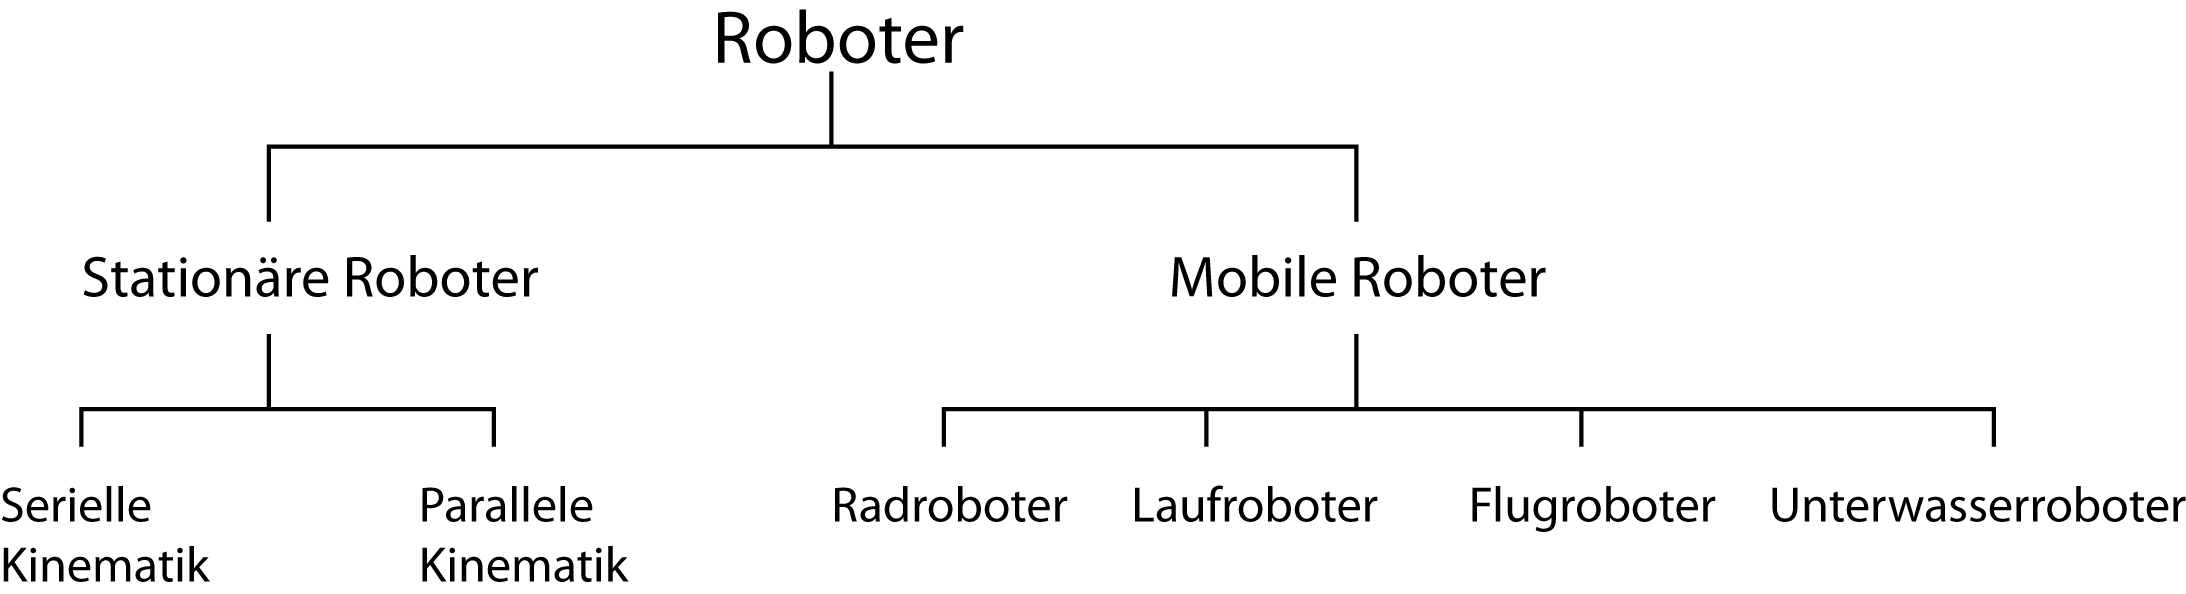
\includegraphics[width=\textwidth]{Bilder/Industrieroboter_unterteilung.png}
%    \caption{Einteilung Roboter \cite[Abbildung~1.1]{wust_grundlagen_2018}}\label{fig:Einteilung_Roboter}
%\end{figure}

%Die Anforderungen an die Automatisierung von Industrierobotern steigen stark. Deshalb ist es notwendig die Robotersteuerungen weiterzuentwickeln, um immer mehr Möglichkeiten zu bieten. Alternativ gibt es auch die Möglichkeit einer modernen Schnittstelle zu bestehender Hardware. Im Folgenden werden die aktuellen Systeme näher erörtert.

%\subsection{Steuerungssoftware} \ver
%Üblicherweise werden Industrieroboter mit der jeweiligen Herstellersoftware angeboten. Die Softwaresteuerung ist bereits auf das Produkt abgestimmt, was dazu führt, dass die Roboter nur schwer mit einer anderen Software verwendbar sind. Dementsprechend ist dieser an einen Hersteller gebunden und ist je nach Anwendung in der Funktionalität eingeschränkt. Der Vorteil liegt darin, dass auftretende Probleme vom Hersteller direkt schnell behoben werden können und die Funktionalität des Industrieroboters in Verbindung mit der Software optimiert wird.

%Um dem Kompatibilitätsproblem zu entgehen, kann man eine Open-Source-Software namens \ac{ROS} Industrial verwenden. Genauer wird dies in \ref{sec:Robot_Operating_System} erläutert. Es gibt nur wenige Open-Source Alternativen zu \ac{ROS}, die lediglich spezielle Anwendungsbereiche abdecken.

%\subsection{Bahnsteuerung} \ver
%Die Ansteuerung eines Punkts im Raum kann auf mehrere Weisen an die Robotersteuerung übergeben werden. Dabei unterscheidet sich die Art der Bewegung des \ac{TCP}. Die zwei folgenden Bahnsteuerungsarten sind die wesentlichen Steuerungsmöglichkeiten für einen Roboterarm, aber hier handelt es sich lediglich um die Grundfunktion, die mit weiteren Methoden verfeinert werden können.
%\begin{description}
%    \item[Point to Point] \textit{\ac{PTP}} ist eine Art der Bewegungsprogrammierung eines Roboterarms, die mit der direkten Verbindung zwischen Start- und Zielkoordinate arbeitet. Man unterscheidet zwischen einer Asynchronen- und Synchronen-\ac{PTP}-Steuerung. Letztere hat den Vorteil, dass die Bewegungen der Achsen gleichzeitig starten und stoppen. Das führt zu einer geringeren Bahnabweichung des \ac{TCP}, dennoch kann die Bahn des Effektors stark von der direkten Verbindungslinie des Start- und Zielpunkts abweichen. Deshalb ist diese Methode nicht für eine Bahnführung mit hohen Genauigkeitsanforderungen geeignet. Der Vorteil liegt in der schnellen und einfachen Bewegungsplanung.

%    \item[Continuous Path] Eine \ac{CP}-Steuerung, auch kartesische Bahnsteuerung genannt, ist eine Methode zur exakten Einhaltung der geforderten Bahn des \ac{TCP}. Dabei werden zwischen Start- und Zielkoordinate sogenannte Interpolationspunkte (Zwischenpositionen) berechnet, denen der Roboterarm folgen soll. Hierfür muss jedoch die passende Roboterstellung in Form von Gelenkwinkeln für jeden Punkt gefunden werden, damit eine gleichmäßige Bewegung des Arms entsteht. Diese Methode eignet sich besonders gut für Aufgaben mit einer hohen Präzisionsanforderung.

%\begin{figure}[ht]
%    \centering
%    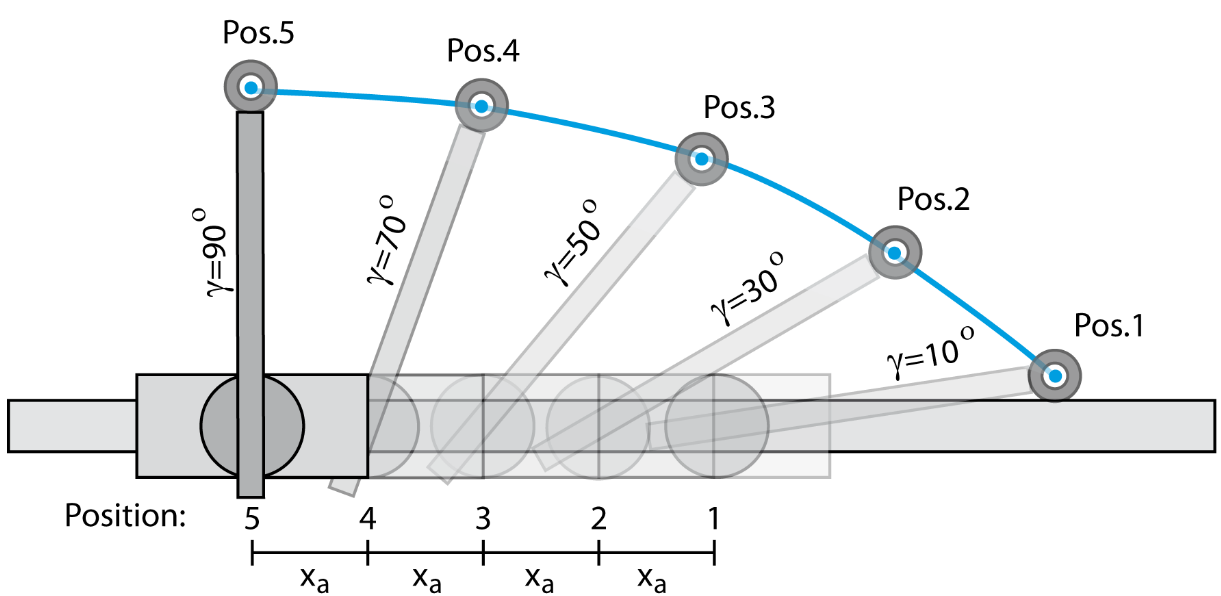
\includegraphics[width=\textwidth]{Bilder/Point_to_Point.png}
%    \caption{\ac{PTP}-Steuerung mit Bahnabweichung \cite[Abbildung~4.3]{wust_grundlagen_2018}}\label{fig:PTP_Steuerung}
%\end{figure} 

%\begin{figure}[ht]
%    \centering
%    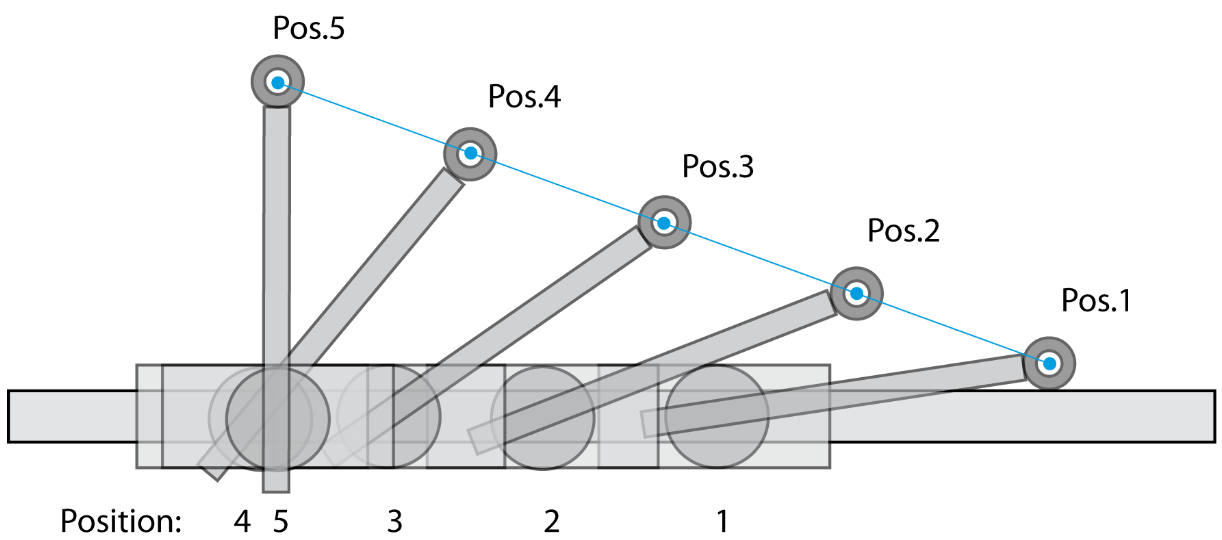
\includegraphics[width=\textwidth]{Bilder/Continuous_Path.png}
%    \caption{\ac{CP}-Steuerung ohne Bahnabweichung \cite[Abbildung~4.4]{wust_grundlagen_2018}}\label{fig:CP_Steuerung}
%\end{figure}
%\end{description} \cite{wust_grundlagen_2018}

\section{Robot Operating System (ROS)} \label{sec:Robot_Operating_System}

Die Kommunikation zwischen in der Robotik eingesetzter Hardware bereitete in der Vergangenheit aufgrund nicht vorhandener Standards bei der Datenübermittlung oft Probleme, die nur mit hohem Entwicklungsaufwand gelöst werden konnten \cite[Kapitel~1]{quigley_ros_2009}. Daher ist ein einheitliches System, das verschiedene Programme und Hardware verbindet, notwendig. Diese Problematik kann durch die Verwendung des \ac{ROS} gelöst werden. Dieses bildet mit einer Vielzahl verfügbarer Pakete eine Grundlage für komplexe Steuerungen. Es kann auf einem einzelnen Computer oder einem Netzwerk aus Computern genutzt werden und vereinfacht die Interoperabilität verschiedener Steuerungshardware. \ac{ROS} dient außerdem als Middleware, die die Kommunikation zwischen Teilen von Software ermöglicht. Die Pakete sind dabei entweder direkt auf \ac{ROS} ausgelegt, oder bilden eine Schnittstelle zu \ac{ROS} für Hardwarekomponenten oder inkompatible Software. Die Website \textit{ros.org} beschreibt das System als ein Paket aus Software und Softwarebibliotheken, mit dem Roboterprogramme entwickelt werden können \cite{rosorg_roshome_2021}.

\ac{ROS} wurde 2007 unter dem Namen \textit{Switchyard} von Morgan Quigley gestartet \cite[Kapitel~1]{joseph_mastering_2018}. Das öffentlich verfügbare \textit{Repository} wurde im Januar 2012 publiziert. Es existieren heute mehrere Konsortien für verschiedene Regionen, darunter beispielsweise das vom Fraunhofer-Institut für Produktionstechnik und Automatisierung geleitete \textit{ROS-I Consortium Europe}. Diese stellen technische Unterstützung und Training für \ac{ROS} bereit und legen Entwicklungsziele fest \cite{rosindustrialorg_brief_nodate}.
Ein großer Vorteil des \ac{ROS} verglichen mit anderen Systemen neben der Hardwareunabhänigkeit ist, dass es ein Open-Source-Projekt ist. Somit kann es gut auf alle Anforderungen angepasst werden und es kann eine Vielzahl an Programmen, die mit \ac{ROS} kompatibel sind, genutzt werden. Dabei ist laut \textit{ros.org} das primäre Ziel des Projekts nicht die Bereitstellung besonders vieler Features, sondern die Unterstützung der Wiederverwendung von Quellcode in der Forschung und Entwicklung \cite[Absatz~2]{dattalo_rosintroduction_2018}.

Nachfolgend werden der Aufbau und die Versionen des \ac{ROS} sowie Möglichkeiten zur Integration einer Objekterkennung beschrieben. Der Fokus liegt auf der im Projekt verwendeten Version ROS-I.

\subsection{Aufbau}

Anders als der Name \ac{ROS} impliziert, handelt es sich technisch gesehen nicht um ein klassisches Betriebssystem, sondern Softwarepakete, die auf bestehenden Betriebssystemen installiert werden können. Das Programm unterstützt offiziell die Linux-Distributionen \textit{Ubuntu} und \textit{Debian}, während für \textit{Windows} und \textit{Arch Linux} experimentelle Versionen zur Verfügung stehen \cite{wikirosorg_noeticinstallation_2020}. Die empfohlene Installationsmethode besteht im Hinzufügen eines Repositorys, wodurch \ac{ROS} über den Paketmanager der verwendeten Linux-Distribution installiert werden kann. Gründe für die Bezeichnung als Operating System sind die Bereitstellung von Services wie Hardware Abstraktion, Paketmanagement sowie eine Kommunikation zwischen Prozessen, wobei es sich um typische Eigenschaften von Betriebssystemen handelt \cite[Absatz~1]{dattalo_rosintroduction_2018}.

\ac{ROS} ist grundsätzlich in mehrere Teile gegliedert. Die offizielle Dokumentation unterscheidet hier zwischen dem ,,Filesystem Level'', ,,Computation Graph Level'' und ,,Community Level'' \cite{romero_rosconcepts_2014}. Für eine bessere Übersicht wird hier zwischen \textbf{Paketmanagement}, \textbf{Struktur} und \textbf{Entwicklung und Dokumentation} unterschieden und verstärkt auf die für diese Arbeit relevanten Teile eingegangen.

\subsubsection{Paketmanagement}

Das Paketmanagement des \ac{ROS} kann in folgende Punkte gegliedert werden:

\begin{description}
    \item[Packages] \textit{Packages} bilden die Grundlage für die Organisation von Softwarekomponenten. Die Softwarepakete enthalten alle notwendigen Teile eines einzelnen Programms. Eine spezielle Art von Packages sind Metapackages, bei denen es sich um eine Zusammenstellung mehrerer Einzelpakete handelt \cite[Absatz~1]{romero_rosconcepts_2014}.
    \item[Repositories] \textit{Repositories} sind Paketquellen, die ein oder mehrere Softwarepakete zum Download bereitstellen. Neben dem primären ROS-\textit{Repository}, das essenzielle Pakete enthält, können Institutionen oder einzelne Entwickler eigene \textit{Repositories} zur Verfügung stellen \cite[Absatz~1/3]{romero_rosconcepts_2014}.
    \item[Dependencies] \textit{Dependencies} sind \textit{Packages}, die von anderen Softwarepaketen zur korrekten Funktionsweise benötigt werden \cite[Absatz~1]{romero_rosconcepts_2014}.
    \item[Workspaces] \textit{Workspaces} sind Ordner im Nutzerverzeichnis des Systems, die bei der Organisation lokal installierter Pakete helfen. Diese fungieren als Overlay über den vom Paketmanager systemweit installierten Softwarepaketen \cite[Absatz~4]{thomas_catkinworkspaces_2017}. Die Priorität liegt hier, wenn Pakete gleichen Namens lokal und systemweit vorhanden sind, bei den lokal installierten Paketen.
    \item[Build System] Für die Installation eigens erstellter Pakete, Software außerhalb der vom Paketmanager nutzbaren \textit{Repositories}, oder lokale Änderungen von Paketen wird für \ac{ROS}-I standardmäßig das Tool \textit{catkin} verwendet, wobei es sich um das offizielle \textit{Build System} von \ac{ROS}-I und einen Nachfolger von \textit{rosbuild} handelt. Im Vergleich zu Tools wie \textit{Autotools} oder dem von catkin unter anderem genutzten \textit{CMake}, zielt \textit{catkin} auf Vereinfachung des Build-Prozesses, Standardisierung bei Verwendung verschiedener Programmiersprachen und das Auflösen von Abhängigkeiten, wodurch der Build-Prozess bei komplexen Zusammenstellungen von Paketen auch von Nutzern mit wenig Programmiererfahrung durchführbar ist \cite[Absatz~1.2]{van_eeden_catkinconceptual_overview_2020}. Pakete für \textit{catkin} werden in \textit{Workspaces} organisiert.
\end{description} 

Das Paketmanagement ähnelt somit dem vieler Linux Distributionen. Pakete werden vorzugsweise direkt über den \textit{Package Manager} des verwendeten Betriebssystems installiert, was auch zur automatischen Installation notwendiger \textit{Dependencies} führt. Bei manuell kompilierten Paketen stellt \ac{ROS} zudem das Programm \textit{rosdep} bereit, mit dem \textit{Dependencies} eines bestimmten Pakets oder mehrere Pakete unter einem gemeinsamen Pfad automatisch installiert werden können \cite[Absatz~2]{loretz_rosdep_2020}.

\subsubsection{Struktur}

\ac{ROS} läuft nicht als ein Prozess, sondern in Form einzelner, verteilter Programme. Neben einer erhöhten Ausfallsicherheit des Gesamtsystems hat diese Struktur weitere Vorteile, wie eine unkomplizierte Verteilung von Prozessen über mehrere Systeme in einem Netzwerk oder die vereinfachte Kommunikation zwischen unabhängig voneinander entwickelten \ac{ROS}-\textit{Packages}. Auch die Möglichkeit, Programme in verschiedenen Programmiersprachen problemlos zu kombinieren ist ein Vorteil dieses modularen Aufbaus. So können viele einzelne, öffentlich verfügbare oder selbst programmierte Pakete zu komplexen Systemen kombiniert werden. 

\begin{description}
    \item[Node] \textit{Nodes} sind logisch zusammenhängende Teile eines Programms. So können Softwarepakete in mehrere Prozesse aufgeteilt werden, die untereinander über den \textit{Master Node} kommunizieren \cite[Absatz~2]{romero_rosconcepts_2014}. Die Kommunikation erfolgt dabei mithilfe von \textit{Messages}.
    \item[Message] Als \textit{Message} wird eine Datenstruktur bezeichnet, die Felder verschiedener, einfacher Datentypen beinhaltet. Dazu gehören beispielsweise \textit{integer, boolean} oder \textit{float} \cite[Absatz~2]{romero_rosconcepts_2014}. Die Kommunikation mittels \textit{Messages} kann auf folgende Arten erfolgen:

        \textbf{Topic}: \textit{Topics} agieren als \textit{Publisher/Subscriber}-System. Nachrichten werden von einem \textit{Node} an ein \textit{Topic} gesendet. Die Identifikation erfolgt hierbei über den Namen des \textit{Topics}. \textit{Nodes} haben die Möglichkeit, ein \textit{Topic} zu registrieren, dessen Nachrichten benötigt werden. Die Anzahl an \textit{Publishern} und \textit{Subscribern}, die den gleichen \textit{Topic} verwenden, ist hierbei nicht limitiert. Auch die Anzahl an \textit{Topics}, die von einem \textit{Node} verwendet werden können, ist unbegrenzt \cite[Absatz~2]{romero_rosconcepts_2014}.
        
        Ein Vorteil dieser Methode ist die Unabhängigkeit zwischen \textit{Publisher} und \textit{Subscriber}. Diese kann aber auch dazu führen, dass ein fehlerhafter \textit{Node} nicht erkannt wird.
        
        \textbf{Service}: Im Vergleich zur einseitigen Kommunikation der \textit{Topics} handelt es sich hier um ein \textit{Request/Reply}-System, wodurch Antworten auf empfangene Nachrichten möglich sind. Ein \textit{Service} besteht aus jeweils einer \textit{Message} für Anfrage und Antwort \cite[Absatz~2]{romero_rosconcepts_2014}.
        
        \textit{Services} eignen sich für die aktive Interaktion zwischen zwei \textit{Nodes}.

    \item[Master] Als \textit{Master} wird der Prozess für die Namensregistrierung und den \textit{Parameter Server} bezeichnet. Dieser ist für die Kommunikation zwischen mehreren \textit{Nodes} zwingend notwendig. Mit dem \textit{Parameter Server} stellt er außerdem globale Konfigurationsdateien bereit \cite[Absatz~2]{romero_rosconcepts_2014}.
\end{description}

\begin{figure}[ht]
    \centering
    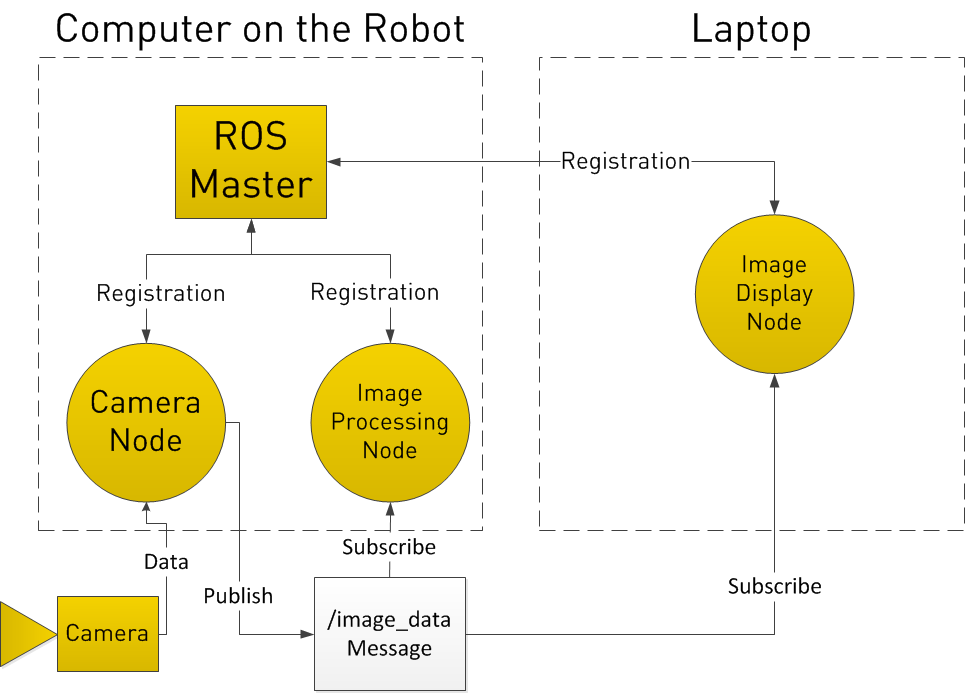
\includegraphics[width=\textwidth]{Bilder/ros_structure.png}
    \caption{ROS Struktur \cite{clearpath_robotics_intro_2015}}
    \label{fig:ros_structure}
\end{figure}

\refFig{fig:ros_structure} zeigt eine mögliche \ac{ROS} Netzwerkstruktur mit Integration einer Kamera und mehreren Computern.

\subsubsection{Entwicklung und Dokumentation}

Da \ac{ROS} von der Community entwickelt wird, sind Ressourcen zum Austausch von Code und Wissen notwendig. Folgendes ist für die Entwicklung besonders relevant:

\begin{description}
    \item[Distributionen] \ac{ROS} ist ähnlich wie Linux-basierte Betriebssysteme in \textit{Distributionen} aufgeteilt. Diese Gliederung sorgt dafür, dass Pakete pro \textit{Distribution} eine bestimmte Softwareversion nutzen \cite[Absatz~3]{romero_rosconcepts_2014}. Dadurch kann eine hohe Kompatibilität zwischen mehreren Paketen gewährleistet werden. Details zu verfügbaren \ac{ROS}-Versionen werden in \refSec{sec:Versionen_ROS} erläutert.
    \item[\ac{ROS} Wiki] Das \textit{\ac{ROS} Community Wiki} ist die Hauptinformationsquelle für Dokumentationen, Tutorials und Korrekturvorschläge \cite[Absatz~3]{romero_rosconcepts_2014}. Einträge können von Jedem nach Erstellen eines Accounts hinzugefügt oder bearbeitet werden. Das \textit{Community Wiki} sollte von Programmierern und Paketerstellern zur Dokumentation genutzt werden.
    \item[Support] Für Neuigkeiten über \ac{ROS} kann das \ac{ROS}-Forum genutzt werden \cite[Absatz~2]{staples_support_2020}. Bei Fehlern, Vorschlägen oder Feature Requests stehen entsprechende Ressourcen zur Eigenrecherche oder Kommunikation zur Verfügung. Aktuelle Links und Leitlinien sind unter \textit{wiki.ros.org/Support} verfügbar \cite[Absatz~3-6]{staples_support_2020}.
\end{description}

\subsection{ROS Versionen} \label{sec:Versionen_ROS}

Wie im letzten Abschnitt erwähnt, gibt es mehrere \ac{ROS}-\textit{Distributionen}. Dabei handelt es sich um Zusammenstellungen von \textit{Packages} miteinander kompatibler Versionen, weshalb sich die Weiterentwicklung der Hauptpakete einer \textit{Distribution} großteils auf Fehlerbehebungen und das Schließen von Sicherheitslücken beschränkt \cite[Absatz~2]{miura_distributions_2021}. Dieses Konzept vereinfacht durch die konstante Code-Basis einer \textit{Distribution} die Entwicklung und Wartung von Softwarepaketen.

Das \textit{Community Wiki} führt Linux als Beispiel für das Konzept der \textit{Distributionen} auf \cite[Absatz~2]{miura_distributions_2021}. Im \ac{ROS}-Kontext sind diese jedoch, besonders bei Betrachtung neuer Versionen, eher mit \textit{Releases} einer einzelnen Linux-Distribution vergleichbar. Frühere \ac{ROS}-Versionen wurden je nach verfügbaren Ressourcen und Nachfrage unterschiedlich lange unterstützt, während aktuelle Releases einen \textit{\ac{LTS}} mit Unterstützungsdauer von fünf Jahren anstreben \cite[Absatz~5]{miura_distributions_2021}. Beim Vergleich zwischen den Daten der Veröffentlichung und Unterstützungsdauer von \ac{ROS} mit den Daten von \textit{Ubuntu LTS} \cite{murray_releases_2021} fallen Parallelen auf. Das Timing der Veröffentlichung neuer \ac{ROS}-Versionen orientiert sich an dem der \textit{Ubuntu LTS}-Versionen.

Da die Aktualisierung der alten Code-Basis von \ac{ROS}-I nicht ohne große Änderungen der Funktionsweise realisierbar ist, wurde 2018 die erste stabile Version von \ac{ROS}-II veröffentlicht. \ac{ROS}-II folgt einem ähnlichen Release-Modell wie die erste Version, wobei die Unterstützungsdauer der jeweiligen Versionen mit ein bis drei Jahren deutlich kürzer ausfällt. Neben den einzelnen Releases gibt es die ,,Rolling Distribution'', die als Version für Entwickler dient und kontinuierlich - auch mit Änderungen, die zu Fehlern im Code führen können - aktualisiert wird \cite{open_robotics_distributions_2021}.

\section{Arten von 3D-Kameras} \ver
Die heutige Arbeit wird in vielen Bereichen durch mobile Roboter sowie stationäre Roboterarme ersetzt. Hierbei spielen vor allem die Genauigkeit sowie die Effizienz eine große Rolle. Die Produktion von Bauteilen, Sortierung, Kartierung und vielen weiteren Arbeitsschritten wurde hauptsächlich durch Kamerasysteme ermöglicht. Diese sind die Augen des Roboters, mit denen der Prozess automatisiert werden kann. Solche Systeme ermöglichen ein autonomes Arbeiten des Roboters und erfordern dadurch zum Beispiel bei einer Qualitätsprüfung, einer Bauteilidentifizierung oder beim Scannen von Produkt-Codes keine Fachkräfte.
Aufgaben, die eine sich ändernde Arbeitsumgebung haben, erfordern eine präzise Umgebungswahrnehmung. Mithilfe einer Kamera kann das Robotersystem so auf veränderte Situationen reagieren. Dadurch steigt zum einen die Flexibilität in Bezug auf die Einsatzbereiche, zum anderen kann durch die Umgebungswahrnehmung so die Wahrscheinlichkeit einer Kollision stark reduziert werden. Beim Einsatz von Kamerasystemen kann man zwischen zwei bekannten Verfahren unterscheiden. Diese werden im folgenden in Bezug auf die Funktion und Einsetzbarkeit verglichen.

\subsection{Stereokamera}\label{sec:Stereokamera} \ver
Die Stereoskopie beschreibt ein Verfahren, welches mithilfe von zweidimensionalen Bildern einen räumlichen Eindruck der Tiefe vermittelt. Eine Stereokamera ist mit zwei nebeneinander angeordneten Kameralinsen ausgestattet. Diese haben einen konstanten Versatz zueinander. Die Verschlüsse der Linsen sind miteinander gekoppelt und müssen nicht individuell eingestellt werden.

Die Funktionsweise der Stereoskopie basiert auf dem binokularen Sehen. Der Ursprung liegt nach Sir David Brewster beim Menschen, indem er das vor ihm liegende Bild durch zwei Augen erkennt und durch die Kombination beider Perspektiven die Tiefen der 2D-Bilder wahrnimmt \cite{sir_david_brewster_stereoscope_1856}. So nimmt die Kamera zwei Bilder aus den jeweiligen Perspektiven der Linsen auf und berechnet mithilfe von Prozessoren und dem mathematischen Verfahren der Triangulierung die Tiefe des zusammengeführten Bildes \cite{waack_stereofotografie_1979}. Dabei muss man jedoch bedenken, dass dieses Verfahren eine hohe Rechenleistung erfordert.

\subsection{RGB-D Kamera}\label{sec:RGB-D_Kamera} \ver
Der Begriff RGB-D beschreibt die Kombination aus einer Farb- und Distanzerkennung. Dabei werden zusätzlich zum einfachen 2D-Farbbild über entsprechende Infrarot-Sensoren die Tiefen gemessen, sodass eine 3D-Aufnahme berechnet werden kann. Dafür wird in der Regel das \ac{ToF} Prinzip genutzt \cite{prof_dr-ing_gunter_pomaska_tiefenkameras_2013}. Dieses sogenannte Laufzeitverfahren misst die Distanzen für jeden Bildpunkt der Szene, indem ein Infrarot-Sensor eine \textit{Point Cloud} auf die Oberfläche projiziert. Die Reflexionen werden von einem CMOS-Bildsensor erkannt. Mit Algorithmen wird die Laufzeit jedes Bildpunktes analysiert und zu Informationen zur Tiefe verarbeitet. Die RGB-Kamera charakterisiert das Bild zusätzlich, um weitere Merkmale festzustellen \cite{prof_dr-ing_gunter_pomaska_tiefenkameras_2013}.

Dadurch, dass die 3D-Aufnahme zusätzlich mit Farbinformationen versehen ist, lassen sich gesamte Szenen und Objekte wesentlich genauer unterscheiden. Bei einer quasi identischen Form können zwei Objekte mit der Farbinformation trotzdem unterschieden werden. Außerdem sind die Anforderungen an Licht- und Umgebungsverhältnisse im Vergleich zur Stereokamera geringer, da die Tiefe mit Infrarot Licht gemessen und nicht berechnet wird. Dennoch sollte genügend Licht für eine saubere Erkennung vorhanden sein. Zudem darf das Sichtfeld der Kamera nicht eingeschränkt werden, damit die Objekte komplett sichtbar sind.

\begin{figure}[ht]
    \centering
    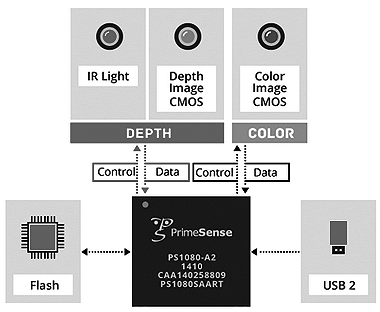
\includegraphics[width=10cm]{Bilder/primeSensor.png}
    \caption{Aufbau RGB-D Kamera \cite{prof_dr-ing_gunter_pomaska_primesensorpng_2013}}
\end{figure}

\section{Objekterkennungsalgorithmen}

Für die Erkennung und Identifikation von Objekten wird ein geeigneter Bild\-erkennungsalgorithmus benötigt. Hauptunterschiede bezüglich der Anwendung sind Genauigkeit, Geschwindigkeit und Hardwareanforderungen im Hinblick auf Leistung. 

Der Algorithmus muss unter den Umgebungsbedingungen des Bauraums zuverlässig funktionieren und ausreichend schnell sein, um keine großen Verzögerungen durch die Erkennung zu verursachen. Die Schnittstelle zu \ac{ROS} muss außerdem die Möglichkeit bieten, Positionsdaten der Objekte an das System weiterzugeben, um die Lokalisierung dieser zu ermöglichen. Die Weitergabe der Tiefenkoordinate durch das Objekterkennungsprogramm ist hierbei optional, da diese auch durch Abgleich der 2D-Koordinaten mit dem Tiefensensor berechnet werden kann. Da in der Arbeit mehrere Objekte verwendet werden, ist zudem die Unterstützung zur Erkennung verschiedener Bauteile im gleichen Bild notwendig.

Die Ansätze von Objekterkennungsalgorithmen können in traditionelle und moderne Ansätze gegliedert werden. Letztere basieren auf \textit{\ac{DL}} und sind grundsätzlich für ein breiteres Spektrum an Objekten geeignet \cite[Absatz~2]{mohan_6_2020}. Folgend werden die Ansätze verglichen und Algorithmen aufgeführt, die gut in \ac{ROS} integrierbar sind und mit RGB-Kamerasystemen funktionieren.

\subsection{Traditionelle Computer Vision}

\textit{\ac{SIFT}} von Lowe \cite{lowe_distinctive_2004} und \textit{\ac{SURF}} von Bay et al. \cite{bay_surf_2006} sind Algorithmen, die auf \textit{Keypoints} in Bildern basieren, welche vom jeweiligen Algorithmus generiert und zur Erkennung von Objekten bei einer bestimmten Übereinstimmungsrate genutzt werden können. \textit{Keypoints} sind um Punkte im Bild, die nahezu invariant gegenüber der Bildparameter wie Vergrößerung, Verzerrung und Rotation sind und somit gut als Orientierungspunkte genutzt werden können \cite[Kapitel~13]{lowe_distinctive_2004}.

Genannte Techniken können für traditionelle Ansätze genutzt werden. Diese funktionieren grundsätzlich folgendermaßen: Zuerst wird die Position der Objekte im Bild durch Scannen des kompletten Bildes näherungsweise bestimmt. Anschließend können Techniken wie beispielsweise \textit{\ac{SIFT}} genutzt werden, um relevante Merkmale der Objekte zu extrahieren. Zuletzt werden Algorithmen wie \textit{\ac{SVM}} \cite{cortes_support-vector_1995} zur Identifikation der Objektkategorie genutzt \cite[Kapitel~1]{youzi_review_2020}. \refFig{fig:detection_traditional} zeigt den beschriebenen Ablauf.

\begin{figure}[ht]
    \centering
    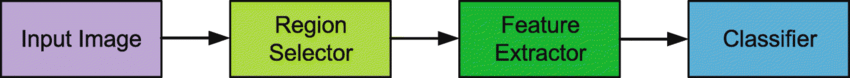
\includegraphics[width=\textwidth]{Bilder/detection_traditional.png}
    \caption{Traditioneller Ansatz \cite[Abbildung~3]{youzi_review_2020}}
    \label{fig:detection_traditional}
\end{figure}

Traditionelle \textit{\ac{CV}} kann durch die geringere Komplexität effizienter als \textit{\ac{DL}} sein. Auch bei Abweichung der zu erkennenden Objekte vom Datensatz, der zum Training des Algorithmus genutzt wird, sind Algorithmen der traditionellen \textit{\ac{CV}} manchmal besser geeignet. Im Gegensatz zu \textit{\ac{DL}} ist traditionelle \textit{\ac{CV}} mit hohem Forschungsaufwand beim Einlernprozess verbunden. \cite[Absatz~2.3]{arai_deep_2020}.

Eine Möglichkeit zur Integration traditioneller Bilderkennung in \ac{ROS} bietet beispielsweise das Paket \textit{find\_object\_2d}, das neben Objektklassifikation und Positionserkennung auch die dreidimensionale Orientierung von Objekten im Raum erkennen kann \cite{labbe_find_2011}.

Aufgrund des Forschungsaufwandes zum Einlernen der Objekte und der hohen Abhängigkeit von der Art und Form zu erkennender Teile eignet sich diese Art der Bilderkennung nur mäßig für den vorliegenden Fall.

\subsection{Deep Learning}

Verglichen mit traditioneller Bilderkennung werden beim \textit{\ac{DL}} keine mathematischen Modelle durch manuelles Sammeln und Auswerten von Prozessdaten (Deskriptive Analytik) oder Erstellen eines prädiktiven Modells (Prädiktive Analytik) erstellt \cite[Kapitel~1]{bonaccorso_machine_2018}. Stattdessen werden \textit{Neural Networks} verwendet. Diese sind mit dem menschlichen Gehirn vergleichbar, da sie aus vielen interagierenden Berechnungszellen bestehen, die zur Entscheidungsfindung miteinander kommunizieren \cite[Kapitel~3~Abschnitt~B]{o_mahony_adaptive_2016}. Dabei fällt der Schritt der Feature-Extraktion weg. Man unterscheidet zwischen \textit{\acp{ANN}}, \textit{\acp{CNN}} und \textit{\acp{RNN}}. Im Rahmen dieser Arbeit wird verstärkt auf die aktuell weit verbreiteten \textit{\acp{CNN}} eingegangen, da diese für viele Anwendungsfälle den besten Kompromiss zwischen Genauigkeit und Geschwindigkeit darstellen.

State of The Art Methoden zur Objekterkennung basieren auf \textit{\acp{DCNN}}. Dabei kann laut Yurtsever et al. zwischen ,,Single Stage Detection Frameworks'', die die Position und Klassifikation simultan durchführen und ,,Region Proposal Detection Frameworks'' unterscheiden werden, bei denen die Kategorisierung in einem zusätzlichen Schritt erfolgt \cite[Kapitel~V,~Absatz~A]{yurtsever_survey_2020}.

Aktuell sind \acp{DCNN} - besonders Single-Stage-Algorithmen - aufgrund der hohen Erkennungsrate in kurzer Zeit besonders relevant. Aufgrund der weiten Verbreitung und somit aktiven Weiterentwicklung, dem vergleichsweise einfachen Prozess zum Einlernen neuer Objekte und einem für das Projekt geeigneten Kompromiss zwischen Geschwindigkeit und Genauigkeit wird hier der Fokus auf den \textit{\ac{YOLO}}-Algorithmus gelegt.

Beim ursprünglich von Redmon et al. entwickelten \textit{\ac{YOLO}}-Algorithmus \cite{redmon_you_2016} handelt es sich um einen \textit{Single-Stage Detector}. Anders als bei \textit{Two-Stage} Algorithmen werden nicht erst Bildabschnitte, die Objekte enthalten könnten, vorgeschlagen. Stattdessen findet die Objekterkennung, -klassifikation und Wahrscheinlichkeitsvorhersage in einem Schritt statt \cite{bandyopadhyay_yolo_2021}. Der Algorithmus teilt Bilder in Regionen auf und erkennt und lokalisiert Objekte in allen Teilen gleichzeitig. Dabei werden sogenannte ,,Bounding Boxes'', die sich mit den Eckpunkten der Objekte decken, generiert \cite[Absatz~2.1.3]{zou_object_2019}.

\begin{figure}[ht]
    \centering
    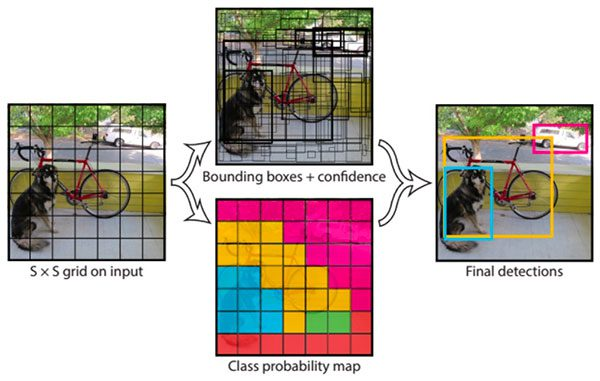
\includegraphics[width=\textwidth]{Bilder/detection_yolo.jpg}
    \caption{Vereinfachte Struktur von YOLO \cite{redmon_you_2016}}
    \label{fig:detection_yolo}
\end{figure}

\refFig{fig:detection_yolo} zeigt die Zerlegung zur Generierung von \textit{Bounding Boxes}. In allen Teilen des Rasters wird eine Objekterkennung und -lokalisierung durchgeführt, auf die die Generierung von \textit{Bounding Boxes} mit Koordinaten relativ zum jeweiligen Teil folgt. Duplikate, die durch über mehrere Teile reichende Objekte entstehen, werden in einem mehrstufigen Prozess mithilfe von \textit{Non-Maximum Suppression} zusammengefasst. \cite[Abschnitt~4]{bandyopadhyay_yolo_2021}

\pagebreak
Ein \textit{\ac{DCNN}} wird hier genutzt, um Bildmerkmale zu extrahieren, was zu einer Verringerung der Auflösung und somit geringeren Ressourcenanforderungen führt \cite[Kapitel~V,~Absatz~A]{yurtsever_survey_2020}. Eine Implementierung des Algorithmus wurde von Redmon selbst unter dem Namen ,,Darknet'' veröffentlicht \cite{redmon_darknet_2021}. Nach der Ankündigung von Redmon, den Algorithmus aufgrund ethischer Bedenken nicht weiterzuentwickeln \cite{joseph_redmon_i_2020}, wurde 2020 eine weitere auf \textit{Darknet} basierende Version von Bochkovskiy et al. veröffentlicht \cite{bochkovskiy_yolov4_2020}.

Im Rahmen dieser Arbeit wird die Version \textit{YOLOv3 Tiny} genutzt. Dabei handelt es sich um eine Version, die speziell auf schwache Hardware ausgelegt ist und somit im Anwendungsfall mit einer hohen Bildwiederholrate betrieben werden kann. Diese ist zur Ermittlung des Objektmittelpunktes bei der Annäherung an die Bauteile vorteilhaft. Die Integration des \textit{Darknet} Frameworks in \ac{ROS} erfolgt mit dem Paket \textit{darknet\_ros} \cite{bjelonic_yolo_2016}.
   \chapter{Software und Hardware}

Folgendes Kapitel umfasst grundlegende Hardwareanforderungen, die verwendete Software und vorbereitende Arbeiten zur Verwendung des Kamerasystems und zum Einlernen benutzerdefinierter Objekte.

\section{Konfiguration des Kamerasystems}

Für die Bearbeitung wurde ursprünglich eine Microsoft Kinect V2 Kamera verwendet. Aufgrund von Hardwarekompatibilitäts- und Treiberproblemen zwischen Kinect und aktueller Hardware und dem schlechten \ac{ROS}-Treibersupport der Kinect für den Anwendungsfall, wurde im späteren Verlauf eine Intel Realsense 435 verwendet. Diese bietet zudem die Möglichkeit einer Befestigung an der Roboterhand. Weitere Tests wurden somit ausschließlich mit der RealSense durchgeführt.

\subsection{Technische Daten}

Folgender Abschnitt behandelt die technischen Daten der Microsoft Kinect V2 und der Intel RealSense 435.

\paragraph{Microsoft Kinect}

Bei der Microsoft Kinect handelt es sich um ein ursprünglich für die Spielkonsole \textit{Xbox} entwickeltes Kamerasystem, das mit einer RGB- und Infrarotkamera zur Tiefenmessung ausgestattet ist. Die RGB-Kamera löst mit $1920 \cdot 1080$ Pixeln auf, die Infrarotkamera mit $512 \cdot 424$. Beide Kameras besitzen eine maximale Bildwiederholrate von 30 Bildern pro Sekunde \cite{sung_real-time_2019}.

\begin{figure}[ht]
    \centering
    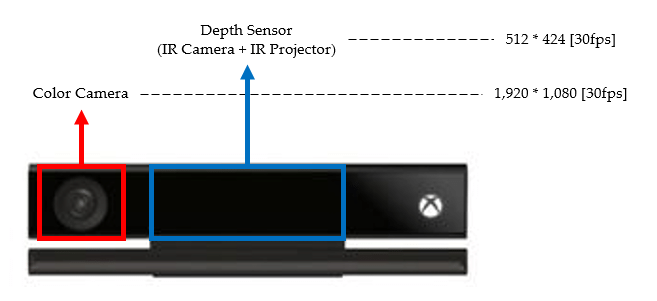
\includegraphics[width=\textwidth]{Bilder/kinect_aufbau.png}
    \caption{Aufbau der Microsoft Kinect v2 \cite[Abbildung~5]{sung_real-time_2019}}
    \label{fig:kinect_aufbau}
\end{figure}

Die Kinect wird aufgrund der vergleichsweise geringen Kosten und der Verfügbarkeit vieler Open-Source-Programme oft in der Forschung der Robotik eingesetzt. Da jedoch kaum Kompatibilität mit aktuellen Systemen vorhanden ist und kein direkter Nachfolger der Kinect V2 existiert, werden jedoch zunehmend andere Kamerasysteme wie die Intel RealSense eingesetzt.

Die minimale Distanz der Kinect V2 beträgt aufgrund der Sättigung des Sensors durch das reflektierte Infrarotlicht ungefähr $0,5m$ \cite[Kapitel~2.1]{noonan_repurposing_2015}. Die Abweichung nimmt mit steigender Entfernung zwischen Kamera und Bauteil leicht zu. Während ein hoher Offset von $-0,02m$ vorhanden ist, beträgt die Standardabweichung auch bei Entfernungen über $1m$ unter $0,002m$, was für den Anwendungsfall ausreichend genau ist \seeFig{fig:kinect_genauigkeit}.

\begin{figure}[ht]
    \centering
    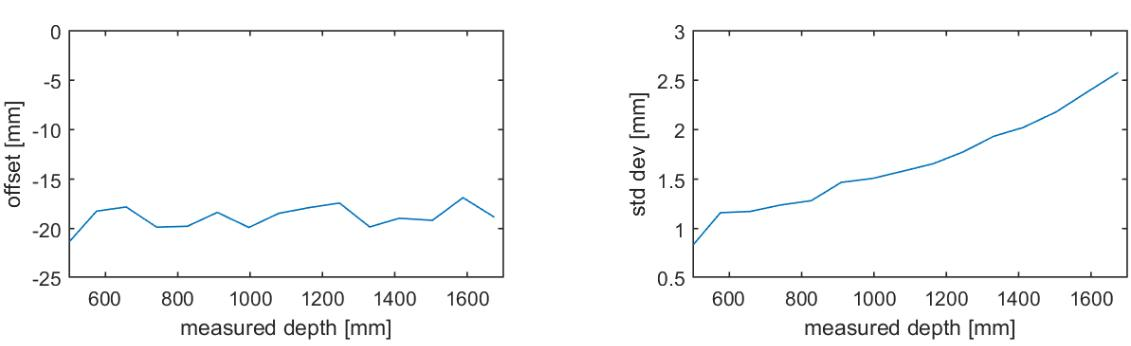
\includegraphics[width=\textwidth]{Bilder/kinect_genauigkeit.jpg}
    \caption{Genauigkeit der Microsoft Kinect v2 \cite[Abbildung~5]{chen_comparison_2017}}
    \label{fig:kinect_genauigkeit}
\end{figure}

Für die Verwendung der Kinect unter Linux-Systemen wird aufgrund der fehlenden offiziellen Herstellerunterstützung der inoffizielle \textit{libfreenect2} Treiber verwendet. Mit diesem können Informationen der RGB- und Infrarotkamera unter Linux ausgelesen werden \cite{xiang_libfreenect2_2016}.
Als Schnittstelle zwischen Kinect und \ac{ROS} Noetic wird das Paket \textit{iai\_kinect2} \cite{wiedemeyer_iai_2021} genutzt. Es stellt neben Funktionen zur Interaktion mit der Kinect über \textit{Topics} Werkzeuge zur Kalibrierung und Anzeige der Kamerabilder zur Verfügung.

\pagebreak
\paragraph{Intel Realsense} \label{subsec:intel_realsense}

Die Intel Realsense 435 hat im Vergleich zur Kinect V2 eine höhere Tiefenauflösung. Im Gegensatz zur Kinect wird hier nicht die \textit{\ac{ToF}}-Technik verwendet, sondern die Tiefe unter Verwendung einer Stereokamera berechnet \seeFig{fig:realsense_aufbau}. 

\begin{figure}[ht]
    \centering
    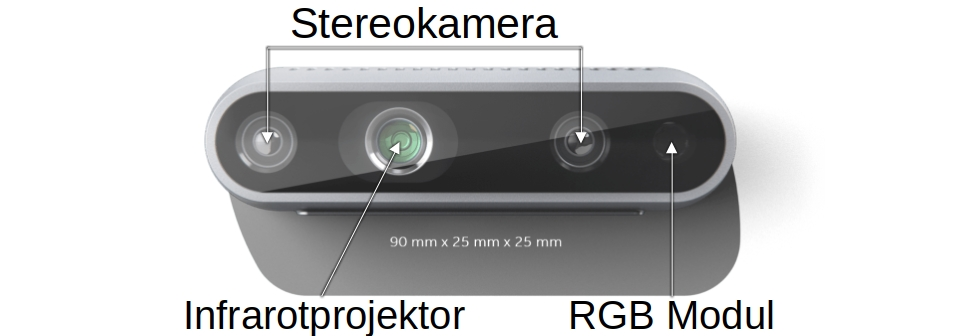
\includegraphics[width=9cm]{Bilder/realsense_aufbau.jpg}
    \caption{Aufbau der Intel RealSense 435, Abbildung nach \cite{intel_corporation_depth_2022}}
    \label{fig:realsense_aufbau}
\end{figure}

Um die Distanzdaten zu ermitteln, ist außerdem ein Infrarotlicht zur Beleuchtung des Aufnahmebereichs integriert, das die Genauigkeit mithilfe der Projektion von Beleuchtungsmustern erhöht \seeFig{fig:realsense_infrarot}. Durch die geringe Baugröße von $90mm \cdot 25mm \cdot 25mm$ und die Kombination Strom- und Datenfluss in einem Kabel kann die RealSense mit geringem Aufwand am Handstück des Roboterarms befestigt werden. Die für Stereokameras typische ungenauere Tiefenmessung im Vergleich zu \ac{ToF}-Systemen wird durch den Infrarotprojektor kompensiert, weshalb die Kamera für diese Anwendung geeignet ist. 

\begin{figure}[ht]
    \centering
    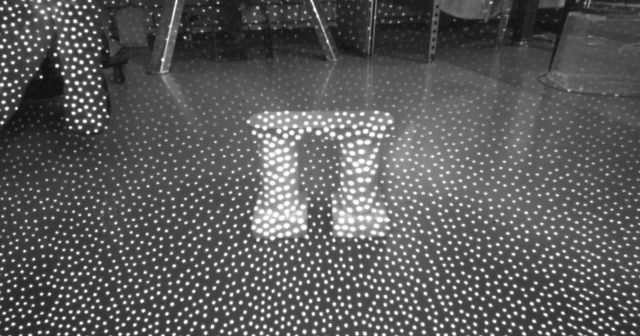
\includegraphics[width=7.12cm]{Bilder/realsense_infrarot.jpg}
    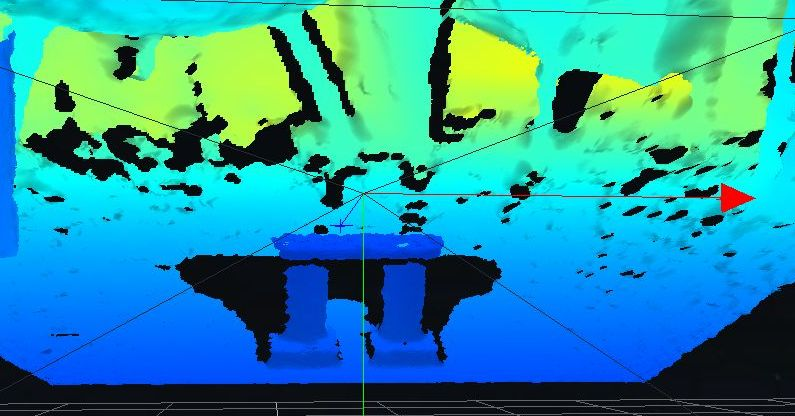
\includegraphics[width=7.14cm]{Bilder/realsense_3d.jpg}
    \caption{Infrarotproj. und 3D-Bild der Intel RealSense 435}
    \label{fig:realsense_infrarot}
\end{figure}

Zur Ermittlung der Genauigkeit wurden Präzisionstests für die Distanz zwischen Kamera und Bauteil durchgeführt. Die Messungen wurden in einem Distanzbereich zwischen $0,3 m$ und $1,0 m$ getätigt, da die minimal mögliche Distanz der RealSense zur Tiefenmessung $0,28 m$ beträgt. Diese Distanz ist auf die Funktionsweise der Stereokamera-Technik zurückzuführen. \refFig{fig:realsense_genauigkeit} zeigt die prozentuale mittlere Abweichung des gemessenen Abstandes zwischen Kamera- und Bauteiloberfläche in Bezug auf den realen Abstand. Dabei überschreitet die Abweichung in keinem Fall $-2 \%$. Bei einem Offset der Messwerte von $+0,001m$ beträgt die maximale Abweichung $\pm1 \%$. Bei geringen Entfernungen ist sie durchschnittlich kleiner. Die im Versuch gemessene Abweichung mit einem Wert von maximal $2\%$ stimmt mit der von Intel angegebenen Genauigkeit überein \cite{intel_corporation_depth_2022}.

\begin{figure}[ht]
    \centering
    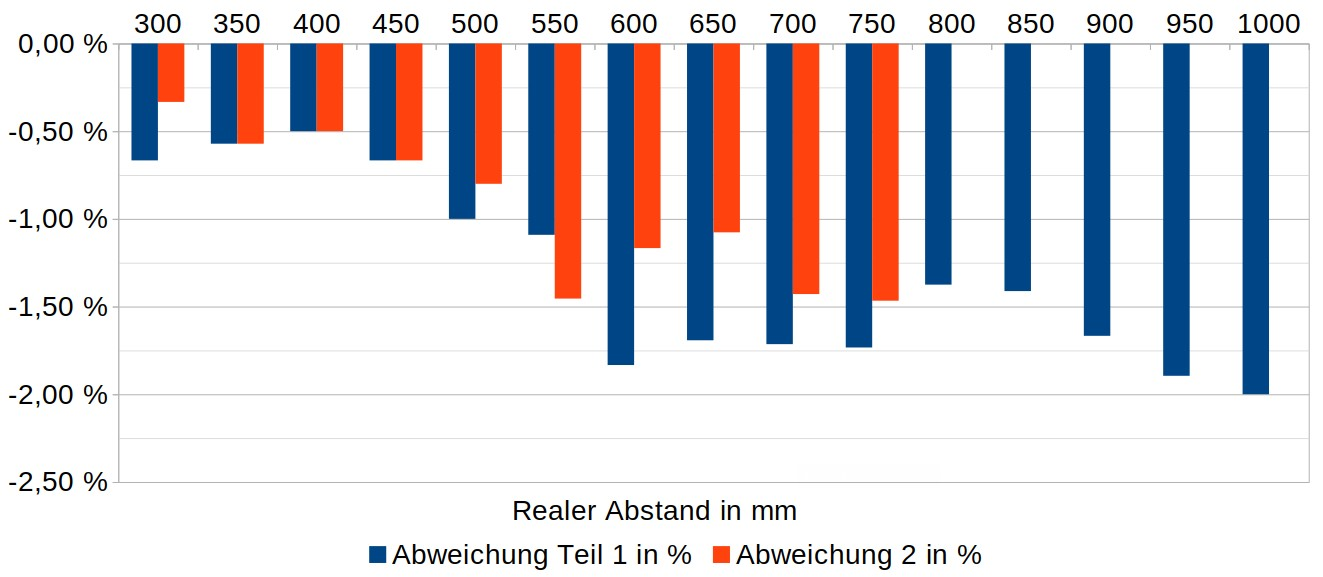
\includegraphics[width=\textwidth]{Bilder/realsense_genauigkeit.jpg}
    \caption{Genauigkeit der Intel RealSense 435}
    \label{fig:realsense_genauigkeit}
\end{figure}

Die Genauigkeit auf planarer Ebene variiert mit Änderung der Entfernung, verschiedenen Bildauflösungen, Version des verwendeten Algorithmus und dem für den Einlernprozess verwendeten Datensatz. Aufgrund der dadurch entstehenden hohen Variabilität sind Tests dieser im Rahmen der Arbeit nicht zielführend. Bei allen durchgeführten Tests war die Erkennung jedoch für den Anwendungsfall mit einer Abweichung von wenigen Millimetern ausreichend genau.

Intel stellt für die Verwendung der RealSense unter Linux das \textit{LibRealSense open source \ac{SDK}} \cite{intel_corporation_intelrealsenselibrealsense_2022} bereit. Mit diesem können, ähnlich wie beim Treiber der Kinect, Daten der RGB-Kamera ausgelesen werden. Die 3D-Daten werden in diesem Fall über eine Kombination der Bilddaten beider Kameras berechnet und nicht wie bei \textit{\ac{ToF}} direkt gemessen. Der Treiber stellt \textit{Point Clouds} - wobei es sich um dreidimensionale, aus einzelnen Punkten zusammengesetzte Bilder handelt - mit optionaler Überlagerung der Farbinformationen zur Verfügung.

Die Integration in das \ac{ROS} erfolgt mit dem offiziellen \textit{realsense-ros} \textit{Package} \cite{intel_corporation_ros_2022}. Dieses stellt die notwendigen \textit{Topics} für die Verwendung des Bilderkennungsalgorithmus und der Abstandsmessung bereit. Dazu zählt neben dem RGB-Bild und den Hardwareinformationen die Integration der \textit{Point Cloud}, mit der der Abstand zwischen Objekt und Kamerasystem bestimmt werden kann \seeFig{fig:realsense_rviz}. Zum Starten des in \textit{realsense-ros} enthaltenen \textit{realsense2\_camera}-Pakets wird eine Konfiguration verwendet, die zum Erreichen einer höheren Kompatibilität mit anderen \ac{ROS}-Paketen die \textit{Point Cloud} nach dem \textit{OpenNI}-Standard bereitstellt \seeAtt{sec:realsense}. Dabei handelt es sich um einen weit verbreiteten, offiziell eingestellten aber weiterentwickelten, Standard zur Verbesserung der Interoperabilität zwischen Software und Hardware \cite{occipital_openni_2022}.

\begin{figure}[ht]
    \centering
    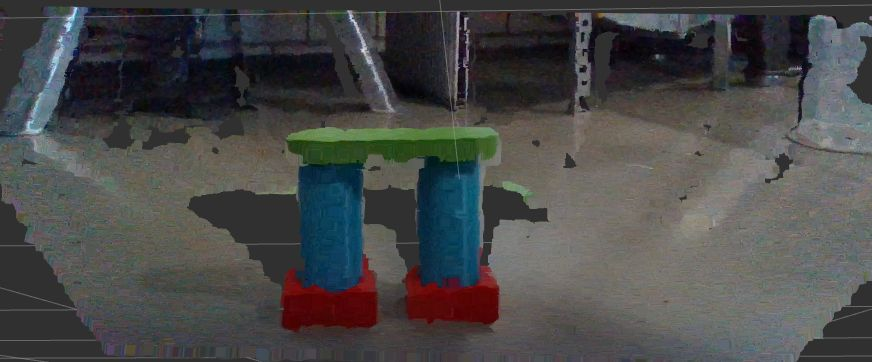
\includegraphics[width=\textwidth]{Bilder/realsense_rviz.jpg}
    \caption{RealSense Point Cloud in Rviz}
    \label{fig:realsense_rviz}
\end{figure}

\subsection{Kalibrierung}

Für die Positionserkennung muss eine Transformation zwischen Roboter- und Kamerakoordinatensystem durchgeführt werden. Diese kann mithilfe einer Hand-Auge-Kalibrierung berechnet werden. Außerdem ist ein Abgleich der Koordinaten zwischen RGB- und Tiefensensor möglich, da durch Ungenauigkeiten bei der Kameraausrichtung und Bildverzerrung Koordinaten in $x$-$y$-Ebene abweichen können. 

\subsubsection{RGB-D Kalibrierung} 

Zum Abgleich zwischen RGB- und Tiefenkamera kann eine RGB-D Kalibrierung durchgeführt werden. 

\paragraph{Microsoft Kinect}

Für die Durchführung mit einer Kinect V2 kann beispielsweise das im Paket \textit{iai\_kinect2} enthaltene Programm zur Kalibrierung genutzt werden \cite{wiedemeyer_iai_2021}. Diese gleicht Abweichungen durch Verzerrung, Rotation und Verschiebung zwischen den Kamerasystemen aus \cite[Beispieldaten]{wiedemeyer_iai_kinect2kinect2_bridgedata_2015}.

Die Kalibrierung erfolgt in diesem Fall mithilfe eines Schachbrett-Musters. Dieses kann bei bekannten Kameraparametern der 2D-RGB-Kamera zur dreidimensionalen Positionsbestimmung eines Objekts im Raum genutzt werden \cite{opencvorg_camera_2019}. Somit ist eine Berechnung der Abweichung zwischen den von den 2D- und 3D-Kameras erkannten Parametern möglich.

\pagebreak
Um die Kalibrierung durchzuführen, wird die Kinect nacheinander in mehreren Positionen relativ zum Kalibrierungsmuster aufgestellt. Nach jeder Bewegung des Musters wird ein Bild mit beiden Kameras der Kinect gemacht, was zum Abgleich genutzt werden kann. Es wird in der Dokumentation von \textit{iai\_kinect2} empfohlen, den Abstand und die Neigung des Kalibrierungsmusters zu verändern, um ein gutes Ergebnis zu erzielen \cite{wiedemeyer_iai_2021}.

\paragraph{Intel RealSense}

Die Intel RealSense ist im Gegensatz zur Kinect bei Verwendung des \textit{iai\_kinect2}-Treibers ab Werk kalibriert. Eine klassische manuelle Kalibrierung ohne spezielle Hardware führt laut Intel mit hoher Wahrscheinlichkeit zu einer Verschlechterung der Kalibrierung. Die aktuelle Firmware der RealSense bietet jedoch Optimierungsmöglichkeiten für diverse Parameter wie Ebenheit der \textit{Point Cloud} oder Distanzgenauigkeit. Diese sind hauptsächlich auf Abnutzungserscheinungen nach längerer Nutzung ausgelegt \cite{grunnet-jepsen_intel_2021}. Da es sich bei der verwendeten RealSense um ein neues Gerät mit ausreichender Genauigkeit handelt \seeFig{fig:realsense_genauigkeit}, wird auf eine Kalibrierung verzichtet.

\subsubsection{Hand-Auge-Kalibrierung}

Als Hand-Auge-Kalibrierung bezeichnet man die Ermittlung von homogenen Transformationsmatrizen zwischen dem Endeffektor des Roboters und dem Kamerasystem sowie die Transformation zwischen Welt- und Basiskoordinatensystem \cite[Kapitel~1]{tabb_solving_2017}.

Man unterscheidet hier zwischen zwei Fällen: Die Kamera kann entweder stationär nahe dem Roboter oder wie im vorliegenden Fall am Endeffektor befestigt werden. Letztere Möglichkeit hat den Vorteil, dass das Kamerasystem durch Anfahren des Bauteilmittelpunktes und mit einer geringen Entfernung zwischen Kamera und Objektoberfläche eine präzisere Steuerung erzielen kann.

Die Kalibrierung in \ac{ROS} kann mit dem \textit{moveit\_calibration}-Paket \cite{rauch_moveit_2022} durchgeführt werden. Dieses unterstützt beide erwähnten Konfigurationsmöglichkeiten. Die vom Programm durchgeführten Messungen erfolgen anhand eines visuellen Kalibriermusters mit distinktiven Formen, mit dem bei bekannter Größe die Lage des Kamerakoordinatensystems bestimmt werden kann. Dazu sollten zum Erfassen mindestens fünf Posen angefahren werden \cite{stechschulte_hand-eye_2022}.

Für den Anwendungsfall dieser Arbeit ist die manuelle Koordinatentransformation ausreichend, da die Lage des Kamerakoordinatensystems im Ursprung der RealSense nur in Relation zum Koordinatensystem, das vom Bewegungsplanungsprogramm von Steinbeck \cite{steinbeck_entwicklung_2022} verwendet wird, berechnet werden muss. Die Koordinatensysteme haben eine rotationsfreie Verschiebung. Die durchgeführte Transformation ist im \refSec{subsec:algorithmus_positionserkennung} näher beschrieben.

\subsection{Befestigung}

Die RealSense kann aufgrund der geringen Baugröße und niedriger Erschütterungsanfälligkeit in der Nähe des Endeffektors am Roboter befestigt werden. Datenübertragung und die Stromversorgung erfolgen über ein einziges USB-Kabel. Aufgrund des größeren Sichtfeldes und besserer Abdeckung des Arbeitsraumes wird die Kamera mit einer Drehung von $90$° gegenüber dem Endeffektor montiert (s. \refFig{fig:realsense_halter}, oben).

\begin{figure}[ht]
    \centering
    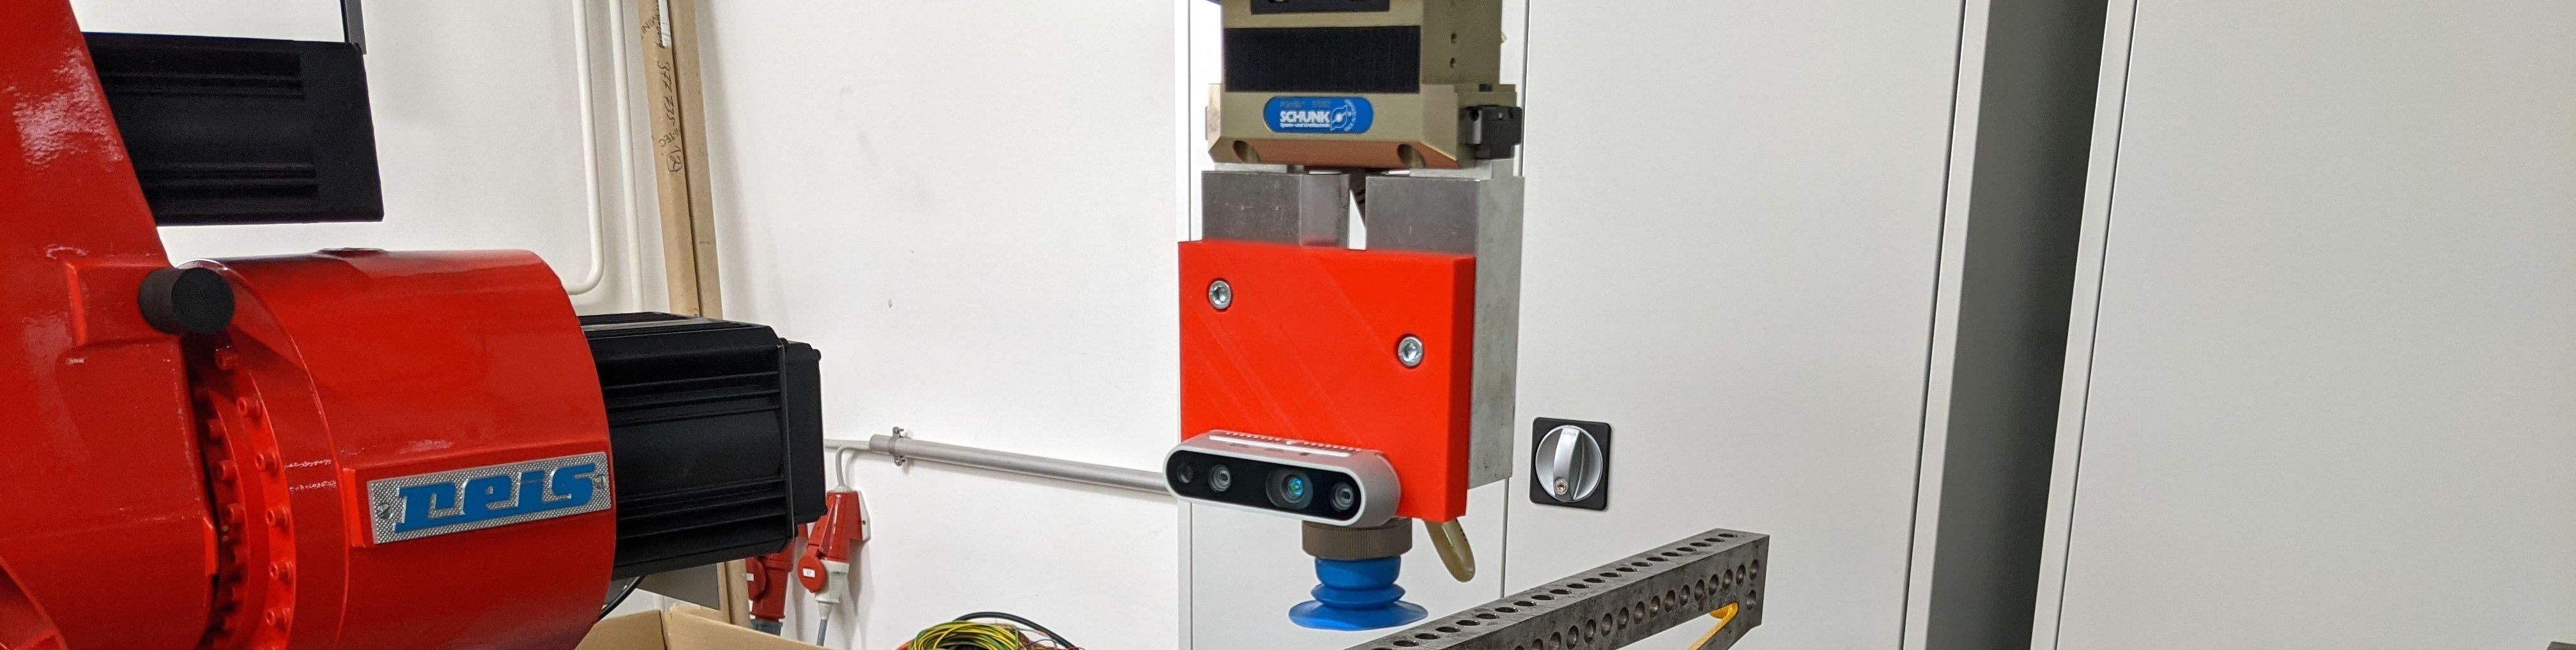
\includegraphics[width=\textwidth]{Bilder/realsense_halter.jpg}
    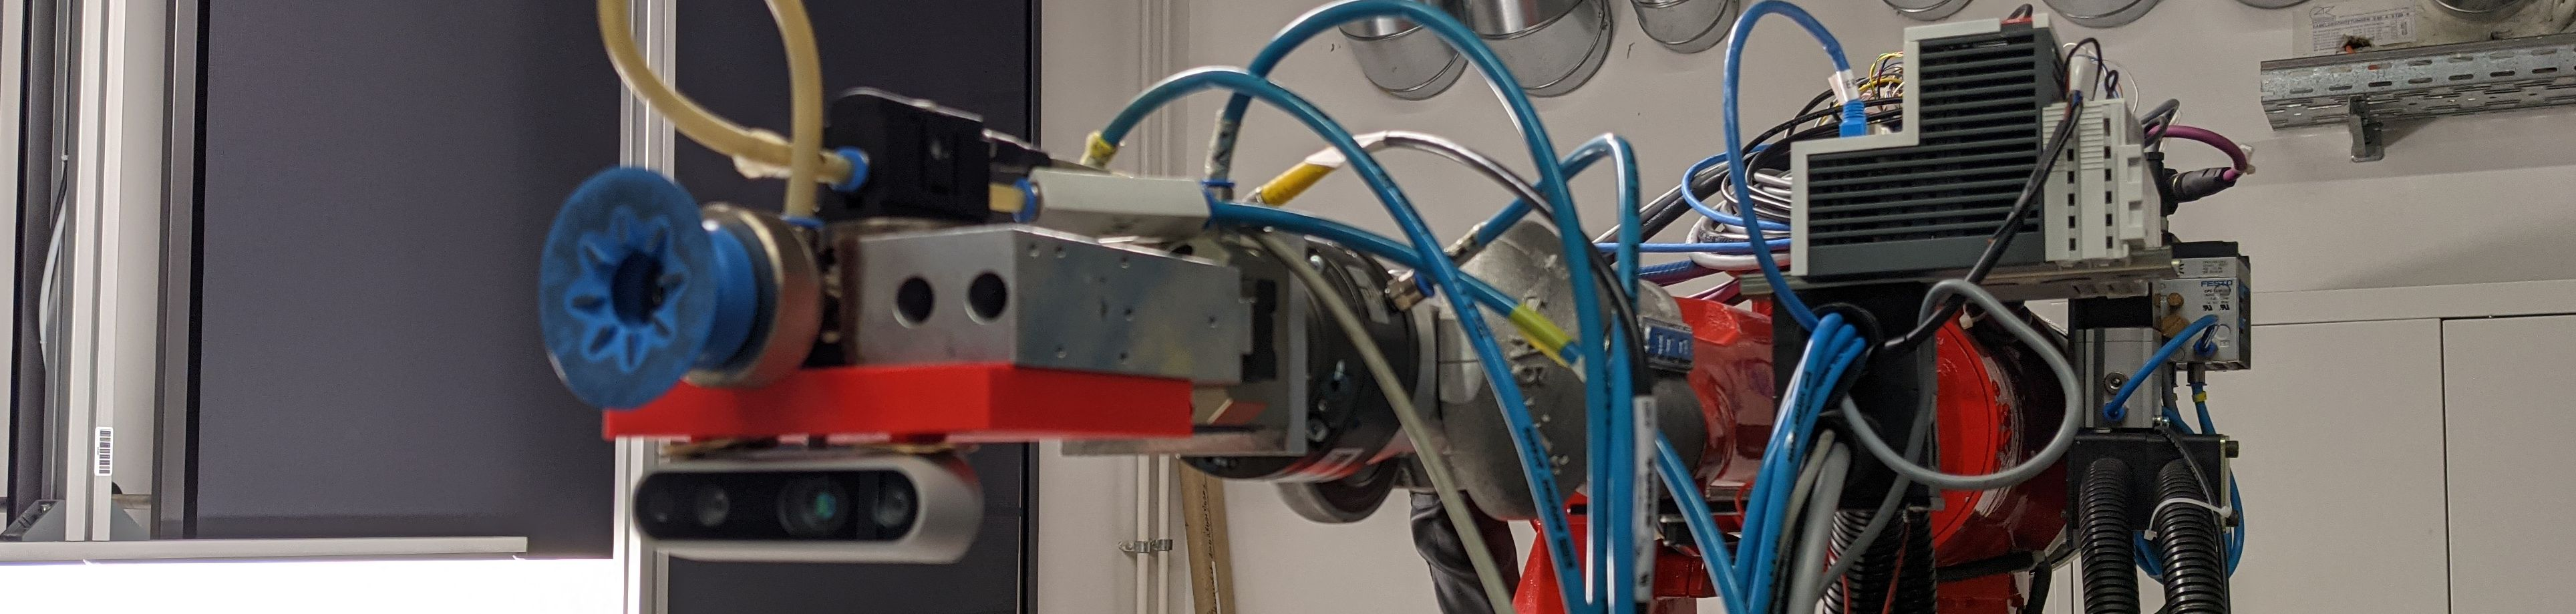
\includegraphics[width=\textwidth]{Bilder/realsense_halter2.jpg}
    \caption{Befestigung der Intel RealSense am Endeffektor}
    \label{fig:realsense_halter}
\end{figure}

\section{Implementierung der Objekterkennung}

\textit{\ac{YOLO}} eignet sich aufgrund schneller und ressourcenschonender Erkennung und Lokalisierung von Objekten ohne große Einschränkungen der Genauigkeit gut für den Anwendungsfall dieser Arbeit. Pro Zelle des Bildrasters können in \textit{YOLOv1} bis zu drei, in \textit{YOLOv3} bis zu neun Objekte gleichzeitig erkannt und lokalisiert werden \cite{bandyopadhyay_yolo_2021}. 

\subsection{Voraussetzungen für das Objekterkennungsprogramm}

Wegen der weitreichenden Kompatibilität und der langen Support-Dauer wird die Version \ac{ROS}-I verwendet. Verglichen mit dem verhältnismäßig neuen \ac{ROS}-II ist ein breiteres Spektrum an kompatibler Hardware und ausgereiften Paketen verfügbar. Bei Noetic handelt es sich um die aktuelle \textit{\ac{LTS}} Version des \ac{ROS}-I-Systems, die bis Mai 2025 unterstützt wird \cite[Abschnitt~3]{miura_distributions_2021}.

\begin{figure}[ht]
    \centering
    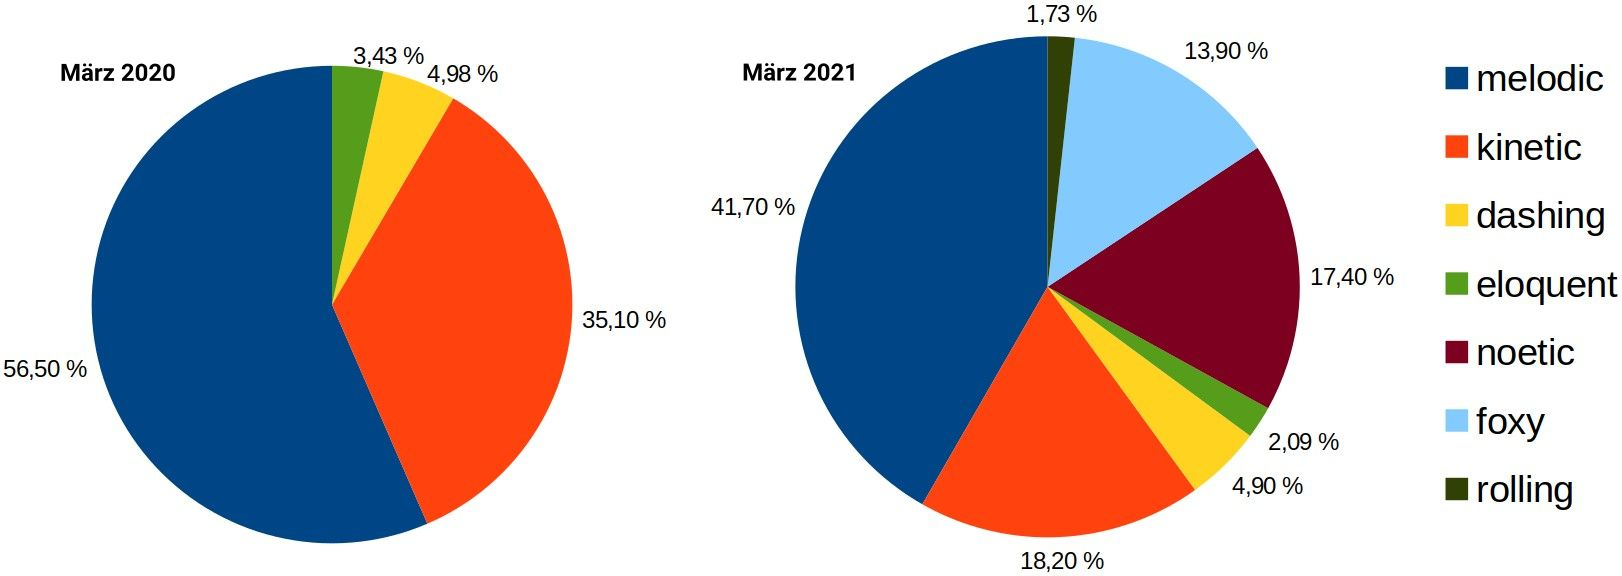
\includegraphics[width=\textwidth]{Bilder/ros_distro_usage.jpg}
    \caption{Anzahl der ROS-Downloads im März 2020 und 2021, Grafik nach \cite{scott_ros_2021}}
    \label{fig:ros_distro_usage}
\end{figure}

%\subsection{Systemanforderungen}

Für die Ausführung von \ac{ROS}-I Noetic wird ein Computer benötigt, der die Hardwareanforderungen von \textit{Ubuntu 20.04 LTS} erfüllt. Bei den Funktionstests wurde ein Computer mit \textit{x86-64}-Architektur verwendet, bei entsprechender Treiberunterstütung des Kamerasystems können aber auch \textit{ARM}-basierte Prozessoren genutzt werden. Für den Einlernprozess der Objekte \seeSec{subsec:add_objects} wird aufgrund der Notwendigkeit von \textit{Nvidia \ac{CUDA}} eine Grafikkarte des Herstellers \textit{Nvidia} benötigt. Zur Objekterkennung ist die Herstellerbindung nicht zwingend, aber für die Verwendung der Hardwarebeschleunigung notwendig. Die Erkennung über den Hauptprozessor des Computers ist somit grundsätzlich möglich, wird jedoch aufgrund der deutlich langsameren Verarbeitung der Objekte nicht empfohlen \cite{bjelonic_yolo_2016}.

%\subsection{Zusätzliche Kernprogramme}

Zur Nutzung des Programms und der Visualisierung werden zusätzlich zum \ac{ROS}-Hauptpaket das 3D-Visualisierungspaket \textit{RViz} \cite{ulisse_perusin_ros-visualizationrviz_2022} und das Bewegungs-planungs-Framework \textit{Moveit} \cite{ioan_a_sucan_moveit_nodate} benötigt. Nähere Informationen zu \textit{MoveIt} sind in der Arbeit von Steinbeck aufgeführt \cite[Abschnitt~3.2]{steinbeck_entwicklung_2022}.


Für die Aufnahme der Objekte müssen deren Art und Position bekannt sein. Durch die Kombination der zwei- und dreidimensionalen Bilddaten kann die Erkennung verschiedener Objekte mithilfe des RGB-Bildes erfolgen. Nach Berechnung des Mittelpunktes der \textit{Bounding Boxes} kann der Abstand zwischen Kamerasystem und der Objektoberfläche mithilfe des 3D-Bildes bestimmt werden. Somit sind alle Koordinaten der vom Greifer anzufahrenden Position bekannt.

\subsection{Training des YOLO-Algorithmus} \label{subsec:add_objects}

Zur Erkennung der in der Arbeit verwendeten Objekte müssen diese durch einen Einlernprozess als sogenannte \textit{Weights} gespeichert werden. Von jedem Objekt werden dazu zuerst mehrere Bilder mit verschiedenen Orientierungen, Lichtverhältnissen und in unterschiedlichen Umgebungen gemacht. Die Genauigkeit steigt üblicherweise mit der Anzahl der Bilder und den Iterationen im Einlernprozess. Diese Bilder müssen anschließend mit \textit{Bounding Boxes} und Objektnamen versehen werden. Die Bounding Boxes werden hier mit dem Programm \textit{LabelImg} \cite{tzutalin_labelimg_2015} erstellt, das das \textit{\ac{YOLO}} Format nativ unterstützt. Sie werden so genau wie möglich auf das Objekt angepasst, sodass die äußeren Punkte die Kanten des Rechtecks berühren. So ist eine möglichst genaue Positionserkennung im späteren Verlauf möglich. Der Datensatz ist unabhängig von der verwendeten \textit{\ac{YOLO}}-Version anwendbar. \refFig{fig:labelimg} zeigt beispielhaft den Aufbau einer Textdatei zur Beschreibung des Labels. Für das Training des neuronalen Netzes wird für jedes Bild eine solche Datei benötigt. Diese setzt sich aus einer Nummer für die Klasse des Objekts, dem Mittelpunkt der \textit{Bounding Box} und der Breite und Höhe dieser zusammen. Die Nummer der Objektklasse richtet sich hier nach der Reihenfolge in einer weiteren Textdatei, die die Klassennamen enthält. Pro Bild können auch mehrere, durch Zeilenumbrüche getrennte, \textit{Bounding Boxes} definiert werden.

\begin{figure}[ht]
    \centering
    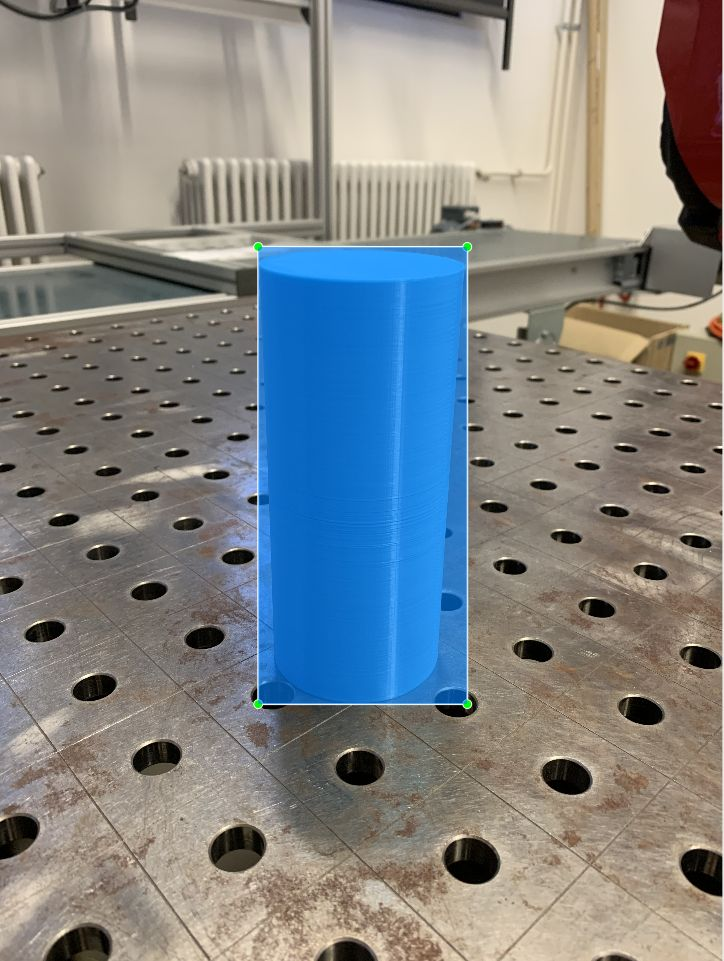
\includegraphics[width=4cm]{Bilder/labelimg.jpg}
    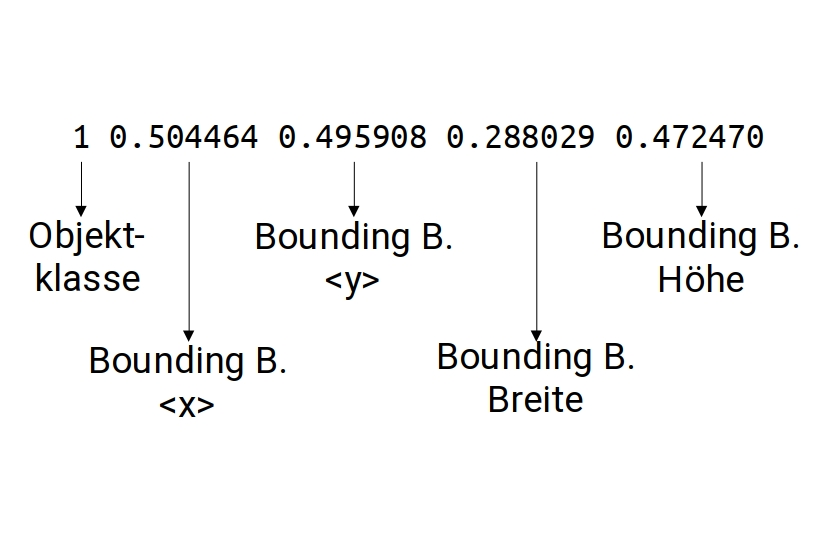
\includegraphics[width=10cm]{Bilder/boundingbox_struktur.jpg}
    \caption{YOLO Label}
    \label{fig:labelimg}
\end{figure}

Das \textit{Darknet} Framework beinhaltet Tools zum Training mit dem durch beispielsweise \textit{LabelImg} erstellten Datensatz. Dieser besteht aus Bildern, in denen ein oder mehrere zu erkennende Objekte enthalten sind und den erwähnten Textdateien mit Informationen über die \textit{Bounding Box}-Positionen. Das Training muss mit der gleichen Version des Algorithmus erfolgen, die später zur Erkennung genutzt wird.

Für das Training des verwendeten \textit{YOLOv3 Tiny}-Algorithmus wurde die in \refAtt{sec:darknet} aufgeführte Konfiguration mit einem Datensatz aus ungefähr 300 Bildern pro Objekt genutzt. Die generierten \textit{Weights} können an die entsprechende Stelle des \textit{rv6l\_3d}-Programms kopiert werden, um eine Objekterkennung zu ermöglichen. Der Einlernprozess wurde nach $10000$ Iterationen gestoppt, da die Genauigkeit bei den verwendeten Objekten mit mehr Wiederholungen nur wenig erhöht wird \seeFig{fig:darknet_iterationen}.

\begin{figure}[ht]
    \centering
    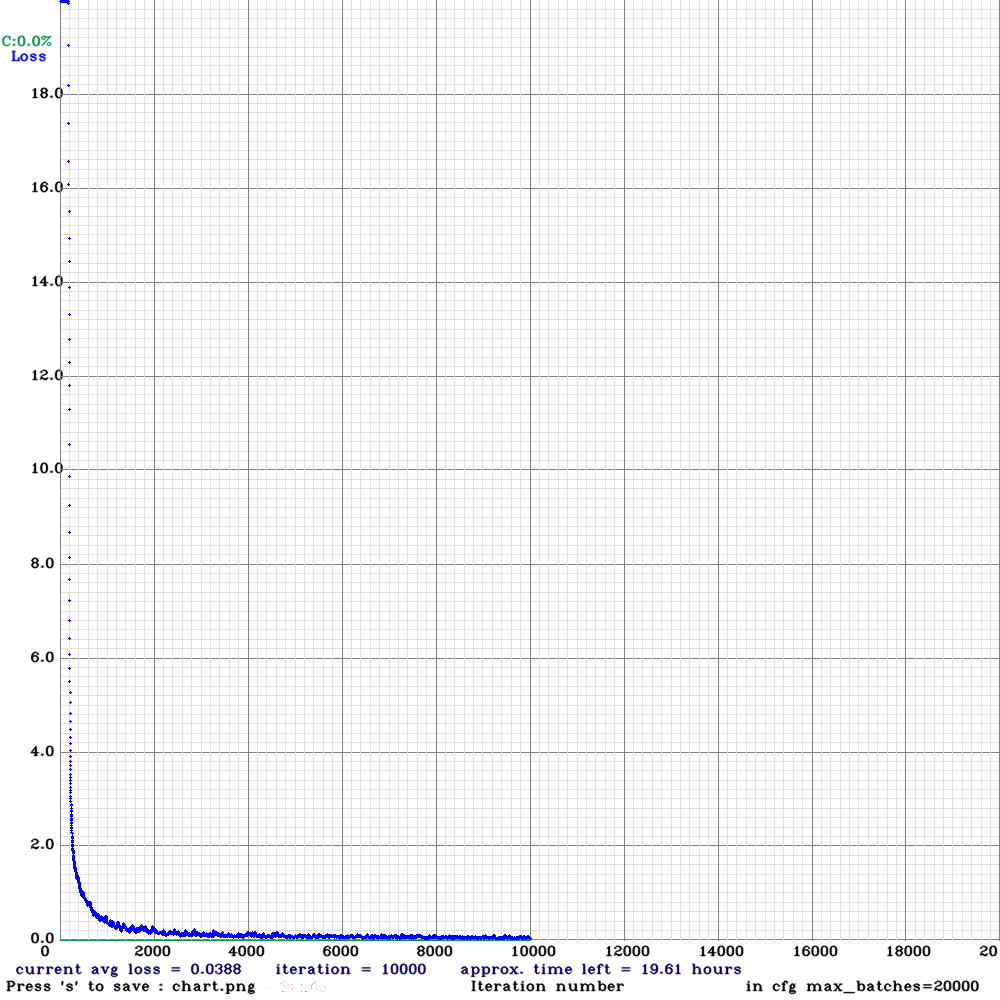
\includegraphics[width=\textwidth]{Bilder/darknet_iterationen.png}
    \caption{Darknet Iterationen [generiert mit Darknet]}
    \label{fig:darknet_iterationen}
\end{figure}

\pagebreak
\subsection{rv6l\_3d-Paket} \label{subsec:rv6l_3d}

Die Grundlage für die Positionserkennung mit \textit{Darknet} in \ac{ROS} bildet das \textit{rv6l\_3d}-Paket \seeAtt{sec:rv6l_3d}. Dabei handelt es sich um ein für diese Anwendung erstelltes Paket für \ac{ROS}, das auf dem 2016 von IntelligentRoboticsLabs veröffentlichten \textit{darknet\_ros\_3d} \cite{intelligentroboticslabs_darknet_ros_3d_2021} basiert. Dieses baut wiederum auf \textit{darknet\_ros} \cite{bjelonic_yolo_2016} auf. Eine Übersicht der Zusammenhänge zwischen den Paketen ist in \refSec{sec:programmstruktur} zu finden. Modifikationen umfassen die Entfernung nicht benötigter Funktionen, eine Mittelpunktberechnung der \textit{Bounding Boxes} und Anpassungen auf das Programm zur Handhabung der Bauteile. Die Kernfunktionalität des \textit{rv6l\_3d}-Pakets besteht in der Bereitstellung dreidimensionaler Objektmittelpunktkoordinaten unter Verwendung einer 3D-Kamera. Das Projekt nutzt die von \textit{darknet\_ros} zur Verfügung gestellten Daten zur Erkennung der planaren Objektposition und gleicht diese mit dem von einer Tiefenkamera gemessenen oder Stereokamera berechneten dreidimensionalen Bild ab, um den Abstand zwischen Kamera und Bauteiloberfläche zu ermitteln.

Die wichtigsten Modifikationen des Pakets umfassen das Entfernen der Marker, die zur Visualisierung der \textit{Bounding Boxes} in \textit{Rviz} dienen, die Berechnung der Objektmittelpunkte sowie Anpassungen des \textit{Topics} mit den Objektpositionen. Somit werden statt vollständigen \textit{Bounding Boxes} die Koordinaten der \textit{Bounding-Box}-Mitten auf der Objektoberfläche in Bezug zum Kamerakoordinatensystem durch den \textit{Publisher} zur Verfügung gestellt. Außerdem wird die Objekterkennung visualisiert \seeFig{fig:rv6l_boxes}.

\begin{figure}[ht]
    \centering
    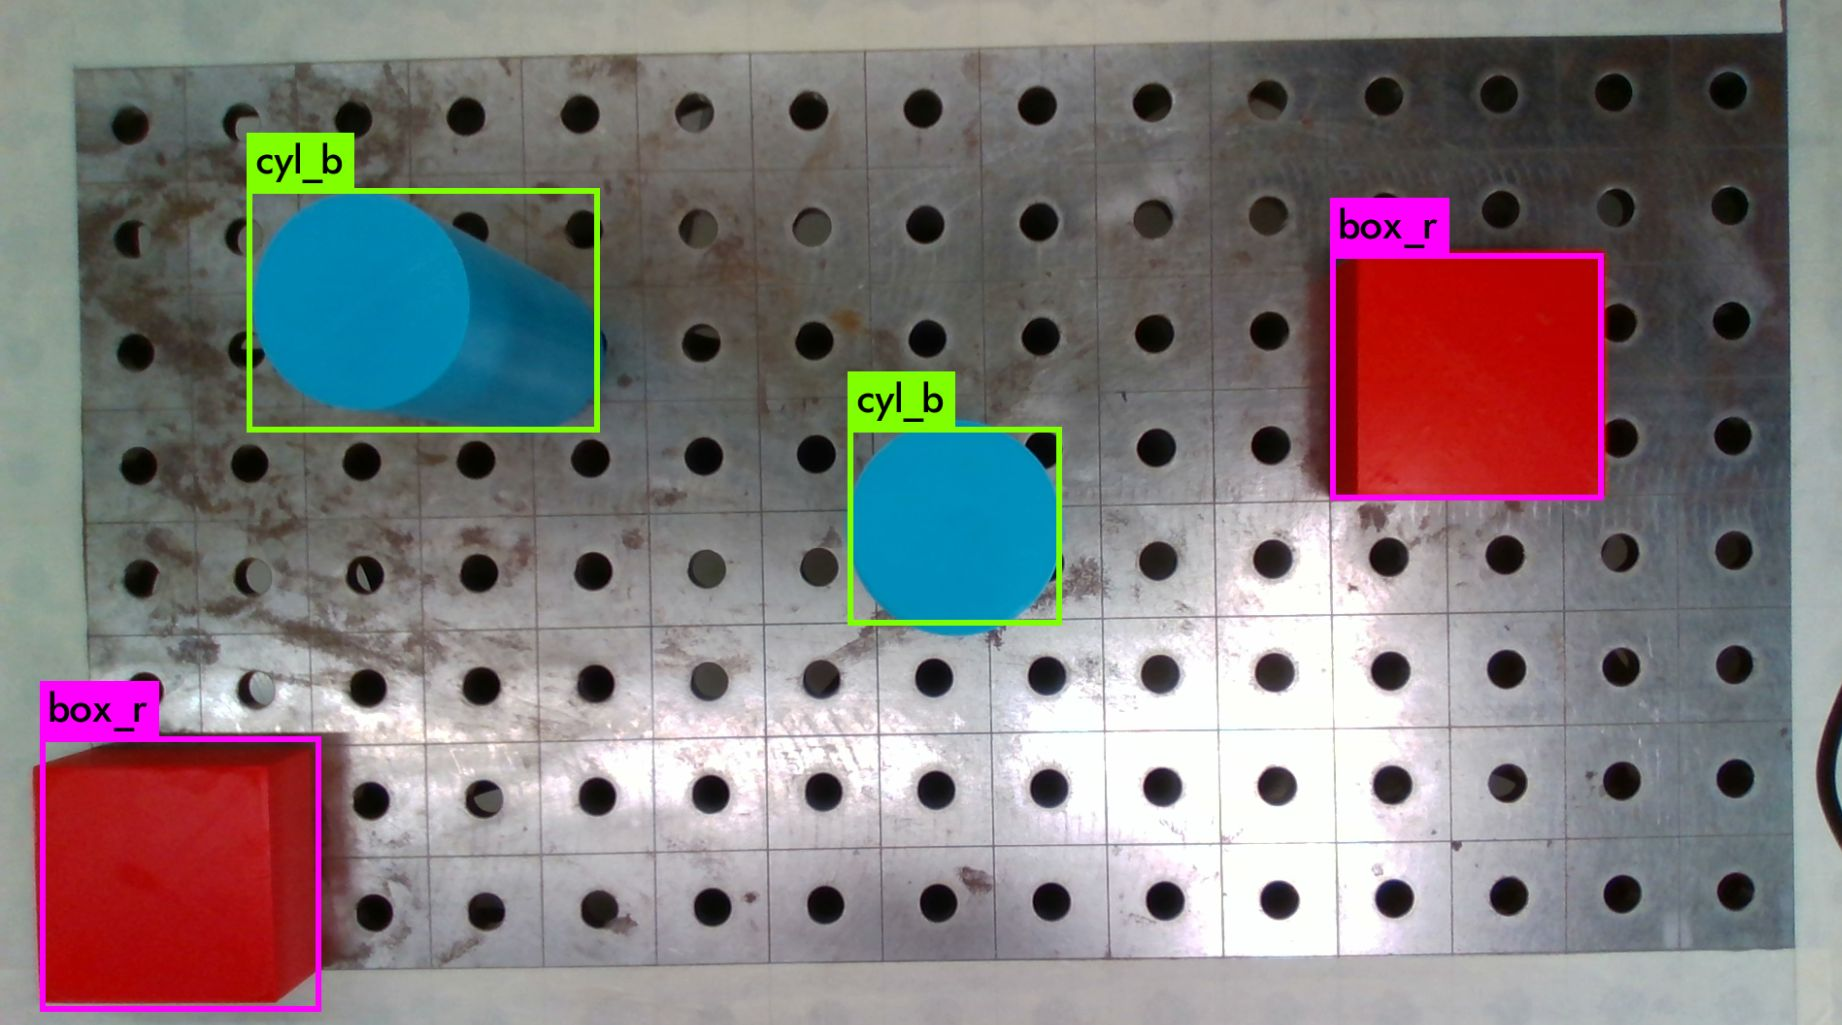
\includegraphics[width=\textwidth]{Bilder/rv6l_boxes.jpg}
    \caption{rv6l\_3d Bounding Boxes}
    \label{fig:rv6l_boxes}
\end{figure}

\newpage
Die Rückgabe des \textit{Bounding Box Publishers} ist im Paket folgendermaßen umgesetzt \seeAtt{sec:rv6l_3d} [C++]:

\begin{lstlisting}[language=c++]
[ . . . ]
        midx = (maxx + minx) / 2; // Objektmittelpunkt (x)
        midy = (maxy + miny) / 2; // Objektmittelpunkt (y)
        midz = (maxz + minz) / 2; // Objektmittelpunkt (z)
      }
    
    rv6l_3d_msgs::RV6L_position bbx_msg;
    bbx_msg.Class = bbx.Class;              // Klasse
    bbx_msg.probability = bbx.probability;  // Wahrscheinlichkeit

    bbx_msg.w = midy; // "horizontale" Position im Bild
    bbx_msg.h = midz; // "vertikale" Position im Bild
    bbx_msg.d = minx; // Abstand (min) durch Point Cloud

    boxes->bounding_boxes.push_back(bbx_msg); // Rueckgabe an BB Message
[ . . . ]
\end{lstlisting}

Die modifizierte \textit{Message} des \textit{rv6l\_3d}-Pakets setzt sich somit aus diesen Werten zusammen:

\begin{lstlisting}[language=python]
string Class         # Objektklasse
float32 probability  # Confidence
float32 w            # horizontale Koordinate im Bild (width)
float32 h            # vertikale Koordinate im Bild (height)
float32 d            # Abstand zum Objektmittelpunkt (depth)
\end{lstlisting}

Es werden Objektklasse, Erkennungssicherheit und die Mittelpunktkoordinaten ausgegeben. Der Datentyp \textit{float32} wird von \textit{C++} und \textit{Python} als \textit{float} interpretiert, weshalb er sich gut für die Übermittlung eignet. Die Koordinaten der Objekte werden relativ zum Kameramittelpunkt unter Berücksichtigung des Abstands zum Objekt in Metern ausgegeben. Dabei ist $w$ in Richtung Bildoberseite und $h$ in Richtung der rechten Bildkante positiv. Der Abstand $d$ beginnt mit $0$ an der Kameraoberfläche und kann nur positive Werte annehmen.
Bei der Abstandsberechnung wird der Abstand zwischen der $h$-$w$-Ebene der Kamera \seeFig{fig:realsense_koord} und der $x$-$y$-Ebene des Basiskoordinatensystems genutzt, sodass dieser unabhängig vom horizontalen Versatz zwischen Objekt und Kamerasystem immer die gleiche Distanz zurückgibt.

\begin{figure}[ht]
    \centering
    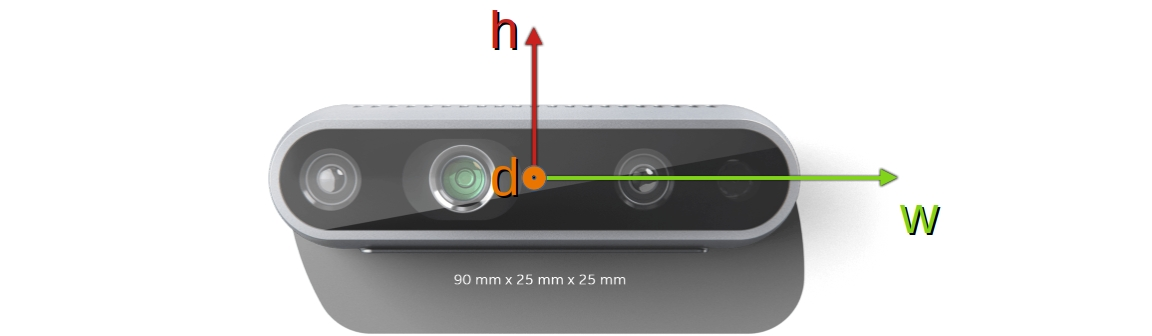
\includegraphics[width=\textwidth]{Bilder/realsense_koord.jpg}
    \caption{Koordinatensystem der Intel RealSense, Abbildung nach \cite{intel_corporation_depth_2022}}
    \label{fig:realsense_koord}
\end{figure}

Das Programm gibt die ermittelten Positionen in Form eines \textit{Topics} an den \textit{Subscriber} des Programms für die Bewegungssteuerung des Roboters weiter:

\subsection{Bounding Box Subscriber}

Der \textit{Subscriber} nimmt die vom \textit{rv6l\_3d} ermittelten Rückgabewerte auf und speichert diese in einer Liste \seeAtt{sec:handhabung} [Python]:

\begin{lstlisting}[language=python]
[ . . . ]
        def callback_pos(self, data):
            for box in data.bounding_boxes:
                self.object_pos_cam = [box.Class, box.h, box.w, box.d]
[ . . . ]
\end{lstlisting}

Diese Liste kann dann vom Bewegungssteuerungsprogramm (basierend auf Steinbeck \cite[Abschnitt~3.5.2]{steinbeck_entwicklung_2022}) zum Anfahren der Zielpositionen genutzt werden. Dieser Algorithmus wurde zur Nutzung mit der Objekterkennung folgendermaßen angepasst:

\subsection{Algorithmus zur Positionserkennung} \label{subsec:algorithmus_positionserkennung}

Für die Positionserkennung müssen die Koordinaten des Objekts in Relation zum Basiskoordinatensystem bekannt sein:
\begin{equation*}
    \tensor[^{G}]{\mathrm{\underline{p}}}{} (G \to Cam) = \tensor[^{G}]{\mathrm{\underline{p}}}{} (G \to Tool) + \tensor[^{G}]{\mathrm{\underline{p}}}{} (Tool \to Cam) 
\end{equation*}

Die aktuelle Transformation vom in \refFig{fig:rv6l_basis} eingezeichneten Koordinatensystem $G$ in das Kamerakoordinatensystem $Tool$ $\tensor[^{G}]{\mathrm{\underline{p}}}{} (G \to Tool)$ kann jederzeit ausgelesen werden. Somit muss für die Bauteilpositionsbestimmung die Transformation $\tensor[^{G}]{\mathrm{\underline{p}}}{} (Tool \to Cam)$ durchgeführt werden. 

\begin{figure}[ht]
    \centering
    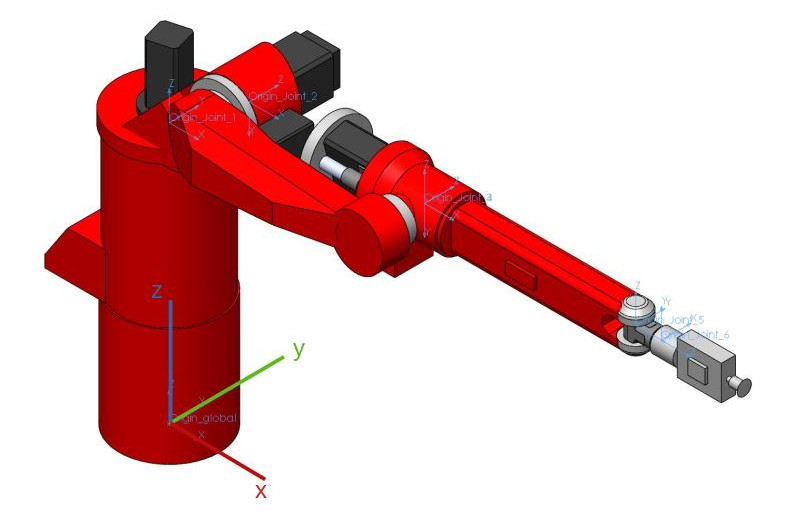
\includegraphics[width=9cm]{Bilder/rv6l_basis.jpg}
    \caption{Koordinatensystem des RV6L, Abbildung nach \cite[Abbildung~12]{leber_steuerung_2021}}
    \label{fig:rv6l_basis}
\end{figure}

Die Tabelle in \refFig{fig:realsense_transformation} zeigt eine Tabelle zur Umrechnung der Orientierungen aller Koordinatensytsteme. Diese gilt ausschließlich für die im Test verwendete Orientierung mit einer Drehung von $90$° gegenüber dem Endeffektor und einer Ausrichtung des Endeffektors parallel zur $x$-Achse und zur $x$-$y$-Ebene \seeFig{fig:realsense_halter}. Dabei ändert sich die Orientierung im Schritt der Bilderkennung des verwendeten Algorithmus nicht, weshalb nur die Translation berechnet werden muss. Diese wird hier als Kameraoffset bezeichnet:

\begin{align*}
    x_{pCam} & = x_{pTool}+o_{x}\\
    x_{pObj} & = x_{pCam}+h_{pObj}\\
    x_{pObj} & = x_{pTool}+o_{x}+h_{pObj}\\\\
    y_{pCam} & = y_{pTool}+o_{y}\\
    y_{pObj} & = y_{pCam}+w_{pObj}\\
    y_{pObj} & = y_{pTool}+o_{y}+w_{pObj}\\\\
    z_{pCam} & = z_{pTool}-o_{z}\\
    z_{pObj} & = z_{pCam}-d_{pObj}\\
    z_{pObj} & = z_{pTool}-o_{z}-d_{pObj}
\end{align*}

Alle Variablen stehen in Bezug zum Koordinatensystem $G$. $[...]_{pCam}$ beschreibt die Position der Kamera, $[...]_{pTool}$ die des Tool-Koordinatensystems und $[...]_{pObj}$ des Objekts. $o_{[...]}$ ist der Offset zwischen Kamera und Tool. 

\begin{figure}[ht]
    \centering
    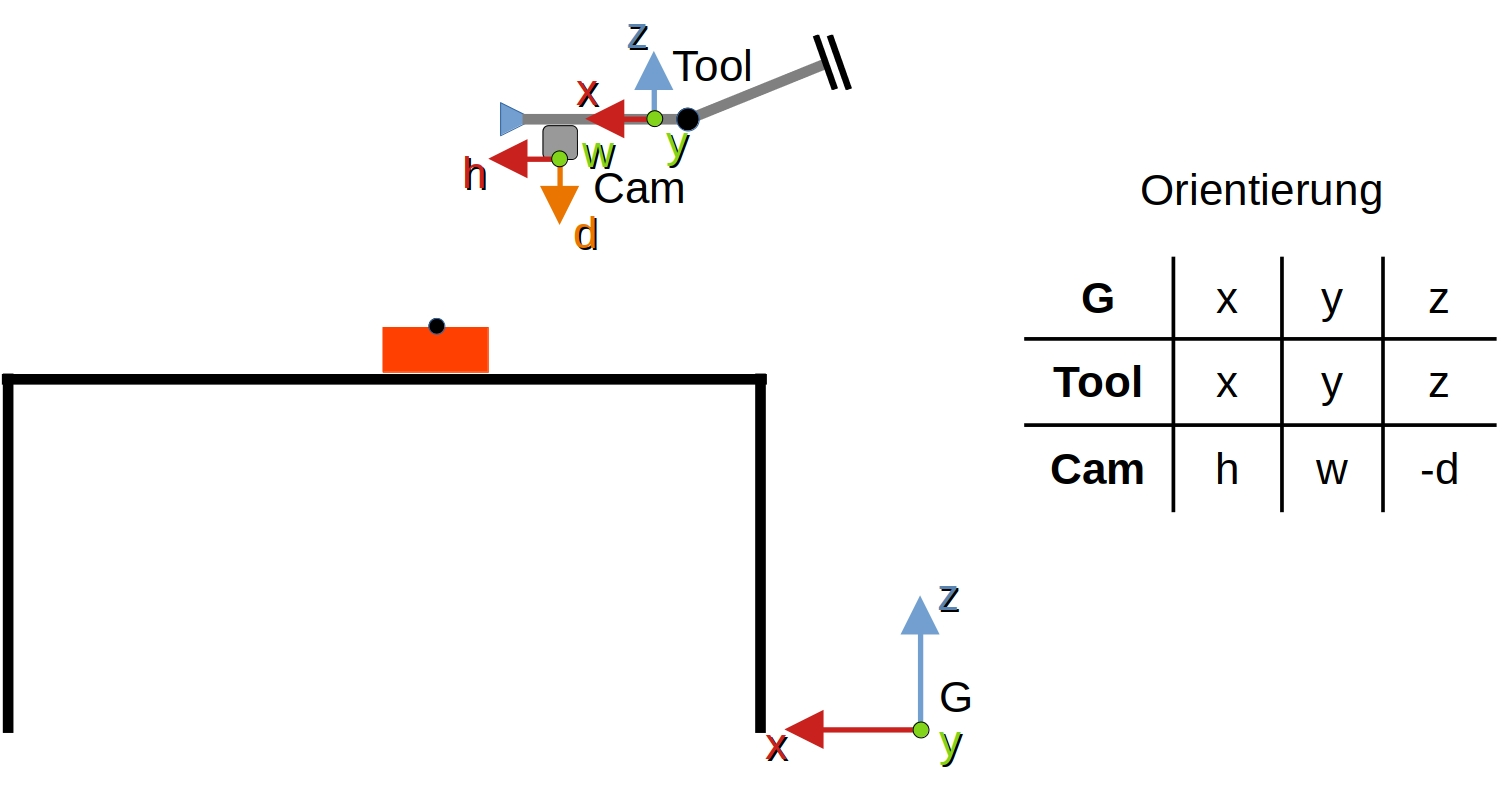
\includegraphics[width=\textwidth]{Bilder/realsense_transformation.jpg}
    \caption{Objektkoordinaten}
    \label{fig:realsense_transformation}
\end{figure}

Die Positionserkennung ist folgendermaßen implementiert [Python]: \footnote[3]{Basiert auf \cite{steinbeck_entwicklung_2022}, \seeAtt{sec:handhabung}. Unwichtige Funktionsaufrufe und -definitionen wurden zur Verbesserung der Übersichtlichkeit entfernt}

\begin{lstlisting}[language=python] 
STATIC_X = 0.237  # Offset in X-Richtung (Greifposition)
STATIC_Y = 0      # Offset in Y-Richtung (Greifposition)
STATIC_Z = 0.237  # Offset in Z-Richtung (Greifposition) = STATIC_X durch Orientierungswechsel
    
SCAN_NEAR = 0.30  # Hoehe fuer nahen Scan
        
[ . . . ]

    py.go_to_scan_pose()  # Scanposition anfahren
    
    ichbinder = uwe() # Klasse aus subscriber_cam initialisieren, Objektpos. auslesen
    rospy.wait_for_message("/darknet_ros_3d/bounding_boxes/", RV6L_positions, timeout=None) # Warten auf Nachricht mit Objektposition relativ zur Kamera
    cam_pos = ichbinder.object_pos_cam  # Aktuelle Position in cam_pos speichern
                         
    py.go_to_scan((cam_pos[1] + REF_X), (cam_pos[2] + REF_Y),(REF_Z - cam_pos[3] + SCAN_NEAR))  # Anfahren der Scanposition ~ ueber dem Bauteil
    
    cam_near = ichbinder.object_pos_cam # Ermitteln des genauen Objektmittelpunktes
        
    py.go_to_pose_goal((cam_pos[1] + REF_X + cam_near[1] + STATIC_X), (cam_pos[2] + REF_Y + cam_near[2] + STATIC_Y), (REF_Z - cam_pos[3] + STATIC_Z - (cam_near[3] - SCAN_NEAR) + 0.25)) # Greifposition anfahren
    
    py.go_to_pose_goal((cam_pos[1] + REF_X + cam_near[1] + STATIC_X), (cam_pos[2] + REF_Y + cam_near[2] + STATIC_Y), (REF_Z - cam_pos[3] + STATIC_Z - (cam_near[3] - SCAN_NEAR))) # Endeffektor absenken
\end{lstlisting}

Der Roboter fährt zuerst in eine Position, die den für die Erkennung nutzbaren Gesamtbereich im Kamerabild sichtbar macht (Zeile 9). Anschließend wird ein Scan durchgeführt und die Objektposition in der Variable \lstinline{cam_pos} gespeichert (Zeile 13). Diese Position ist im Kamerakoordinatensystem \seeFig{fig:realsense_koord} angegeben. Aufgrund der Perspektive und der Funktionsweise der \textit{Bounding Boxes} weicht der Mittelpunkt jedoch vom realen Bauteilmittelpunkt ab. Diese Abweichung ist in \refFig{fig:rv6l_boxes} erkennbar.

Wegen der Abweichung wird diese ungefähre Mittelpunktposition mit dem Mittelpunkt der Kamera in der $x$-$y$-Ebene $30cm$ über dem Bauteil angefahren. Dadurch ist nur noch die Objektoberseite sichtbar, sodass der genaue Objektmittelpunkt bestimmt werden kann (Zeile 15). Zum Ermitteln der Zielkoordinaten werden die Startkoordinaten und die von der Kamera ermittelten Objektkoordinaten gemäß der in \refFig{fig:realsense_transformation} dargestellten Umrechnungstabelle addiert. Außerdem werden $30cm$ (Variable \lstinline{SCAN_NEAR}) zum Anfahren der korrekten Höhe zur $z$-Koordinate addiert. Der Kameraversatz ist in diesem Fall irrelevant, da er in Start- und Zielposition den gleichen Wert hat und somit eliminiert wird. Somit bewegt sich die am Endeffektor befestigte Kamera beim Aufruf der Funktion \lstinline{go_to_scan} zum ungefähren Objektmittelpunkt. Nach Anfahren dieser Koordinaten wird der Mittelpunkt des Objekts erneut ermittelt und in der Variable \lstinline{cam_near} gespeichert (Zeile 17). Dazu wird das Kamerakoordinatensystem verwendet, wodurch nur die Abweichung zwischen Kamera- und Bauteilmittelpunkt gespeichert wird.

Zum Greifen des Bauteils muss der Versatz und die Rotation zwischen Kamera und Endeffektor beachtet werden. Die Variablen \lstinline{STATIC_<...>} legen diesen Offset zwischen Kamera und $Tool$-Koordinatensystem fest. Sie unterscheiden sich je nach Roboterkinematik und Kameraposition. Im Test wurde die Intel RealSense mit einem Offset von $23,7cm$ in $x$-Richtung und $-5,7cm$ zur Vorderkante der Kamera in $z$-Richtung des $Tool$-Koordinatensystems montiert. Somit wird mit \lstinline{STATIC_X} die $x$-Koordinate der anzufahrenden Position um $23,7cm$ erhöht, damit das $Tool$-Koordinatensystem in der Greifposition sich mit der $x$-Koordinate der Kamera in der Scanposition deckt. Im vorliegenden Fall ist aufgrund des Orientierungswechsels zwischen Scan- und Greifposition der Versatz zwischen Kamera und $Tool$ von $23,7cm$ in $x$-Richtung äquivalent zum Versatz der Scanposition in $z$-Richtung \seeFig{fig:rv6l_positionen}. Der Kameraoffset kann beispielsweise durch Messungen am realen System ermittelt werden. Im angefügten Quellcode wurde der Wert \lstinline{STATIC_Z} durch experimentelle Annäherung leicht angepasst.

\begin{figure}[ht]
    \centering
    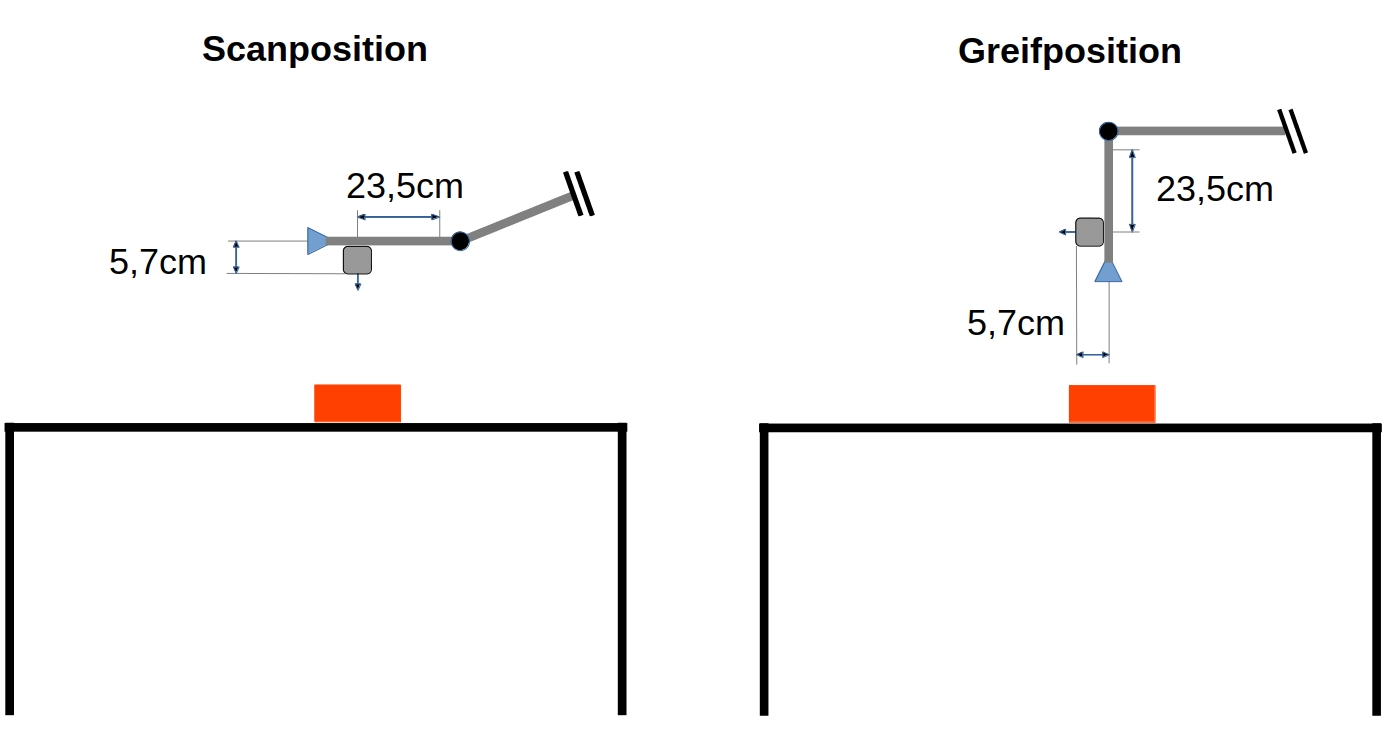
\includegraphics[width=\textwidth]{Bilder/rv6l_positionen.jpg}
    \caption{Roboterpositionen}
    \label{fig:rv6l_positionen}
\end{figure}

Im nächsten Schritt wird die Funktion \lstinline{go_to_pose_goal} aufgerufen (Zeile 19). Diese fährt die Zielposition im Gegensatz zur \lstinline{go_to_scan}-Funktion nicht in \mbox{Scan-,} sondern in Greifposition an. Somit erfolgt hier der erwähnte Orientierungswechsel. Als Zielkoordinaten werden hier sowohl die in \lstinline{cam_near} gespeicherten genauen Offset-Werte für den Bauteilmittelpunkt, die anzufahrende Höhe von $25cm$ vor Absenken des Endeffektors, als auch die Werte der \lstinline{STATIC_[...]}-Variablen zu den anfangs ermittelten Koordinaten addiert, wodurch die genaue Zielposition angefahren wird. Im letzten Schritt wird der Greifer um die erwähnten $25cm$ abgesenkt, um das Bauteil zu greifen.

   \chapter{Gesamtsystem}

Das Gesamtsystem besteht softwareseitig aus einer Kombination öffentlich verfügbarer und eigens erstellter \ac{ROS}-Pakete. Das Programm ist so gestaltet, dass die Roboter- und Bilderkennungshardware, wenn passende Konfigurationsdateien für Kamerasystem und Roboterspezifikation vorhanden sind, variabel sind. Folgendes Kapitel bietet einen Überblick über die Aufgaben aller verwendeten Pakete und die Struktur des gesamten Systems mit Fokus auf der Objekterkennung sowie den zeitlichen Ablauf eines einzelnen Bewegungsschrittes.

\textbf{Hinweis}: Das in diesem Kapitel beschriebene Gesamtsystem ist noch nicht vollständig implementiert. Die Ansteuerung des Greifers ist aufgrund von Kommunikationsproblemen mit der verwendeten Reis Robotersteuerung nicht funktionsfähig und muss somit manuell bedient werden. Die Schnittstelle zwischen der Objekterkennung und Handhabung funktioniert aktuell ausschließlich, wenn nur ein einzelner beliebiger Block vom Kamerasystem erkannt wird. Zu Demonstrations- und Testzwecken werden daher zwei Algorithmen zur Verfügung gestellt: für die intelligenten Handhabungssequenzen der Teile wird ein fester Bauplan für Start- und Zielposition vorgegeben\aus.
Zur Nutzung der Bilderkennung in Verbindung mit der Bewegung der Objekte wird der in \refSec{subsec:algorithmus_positionserkennung} beschriebene Algorithmus genutzt.


\section{Programmstruktur} \label{sec:programmstruktur}

Die Zusammenhänge aller Programme sind in \refFig{fig:gesamtsystem_struktur} aufgeführt. Hier wird verstärkt auf die Objekterkennung (rot) eingegangen. Die Roboterbewegung wird in einer Arbeit von Steinbeck \cite[Abschnitt~4.1]{steinbeck_entwicklung_2022} behandelt.

\begin{figure}[ht]
    \centering
    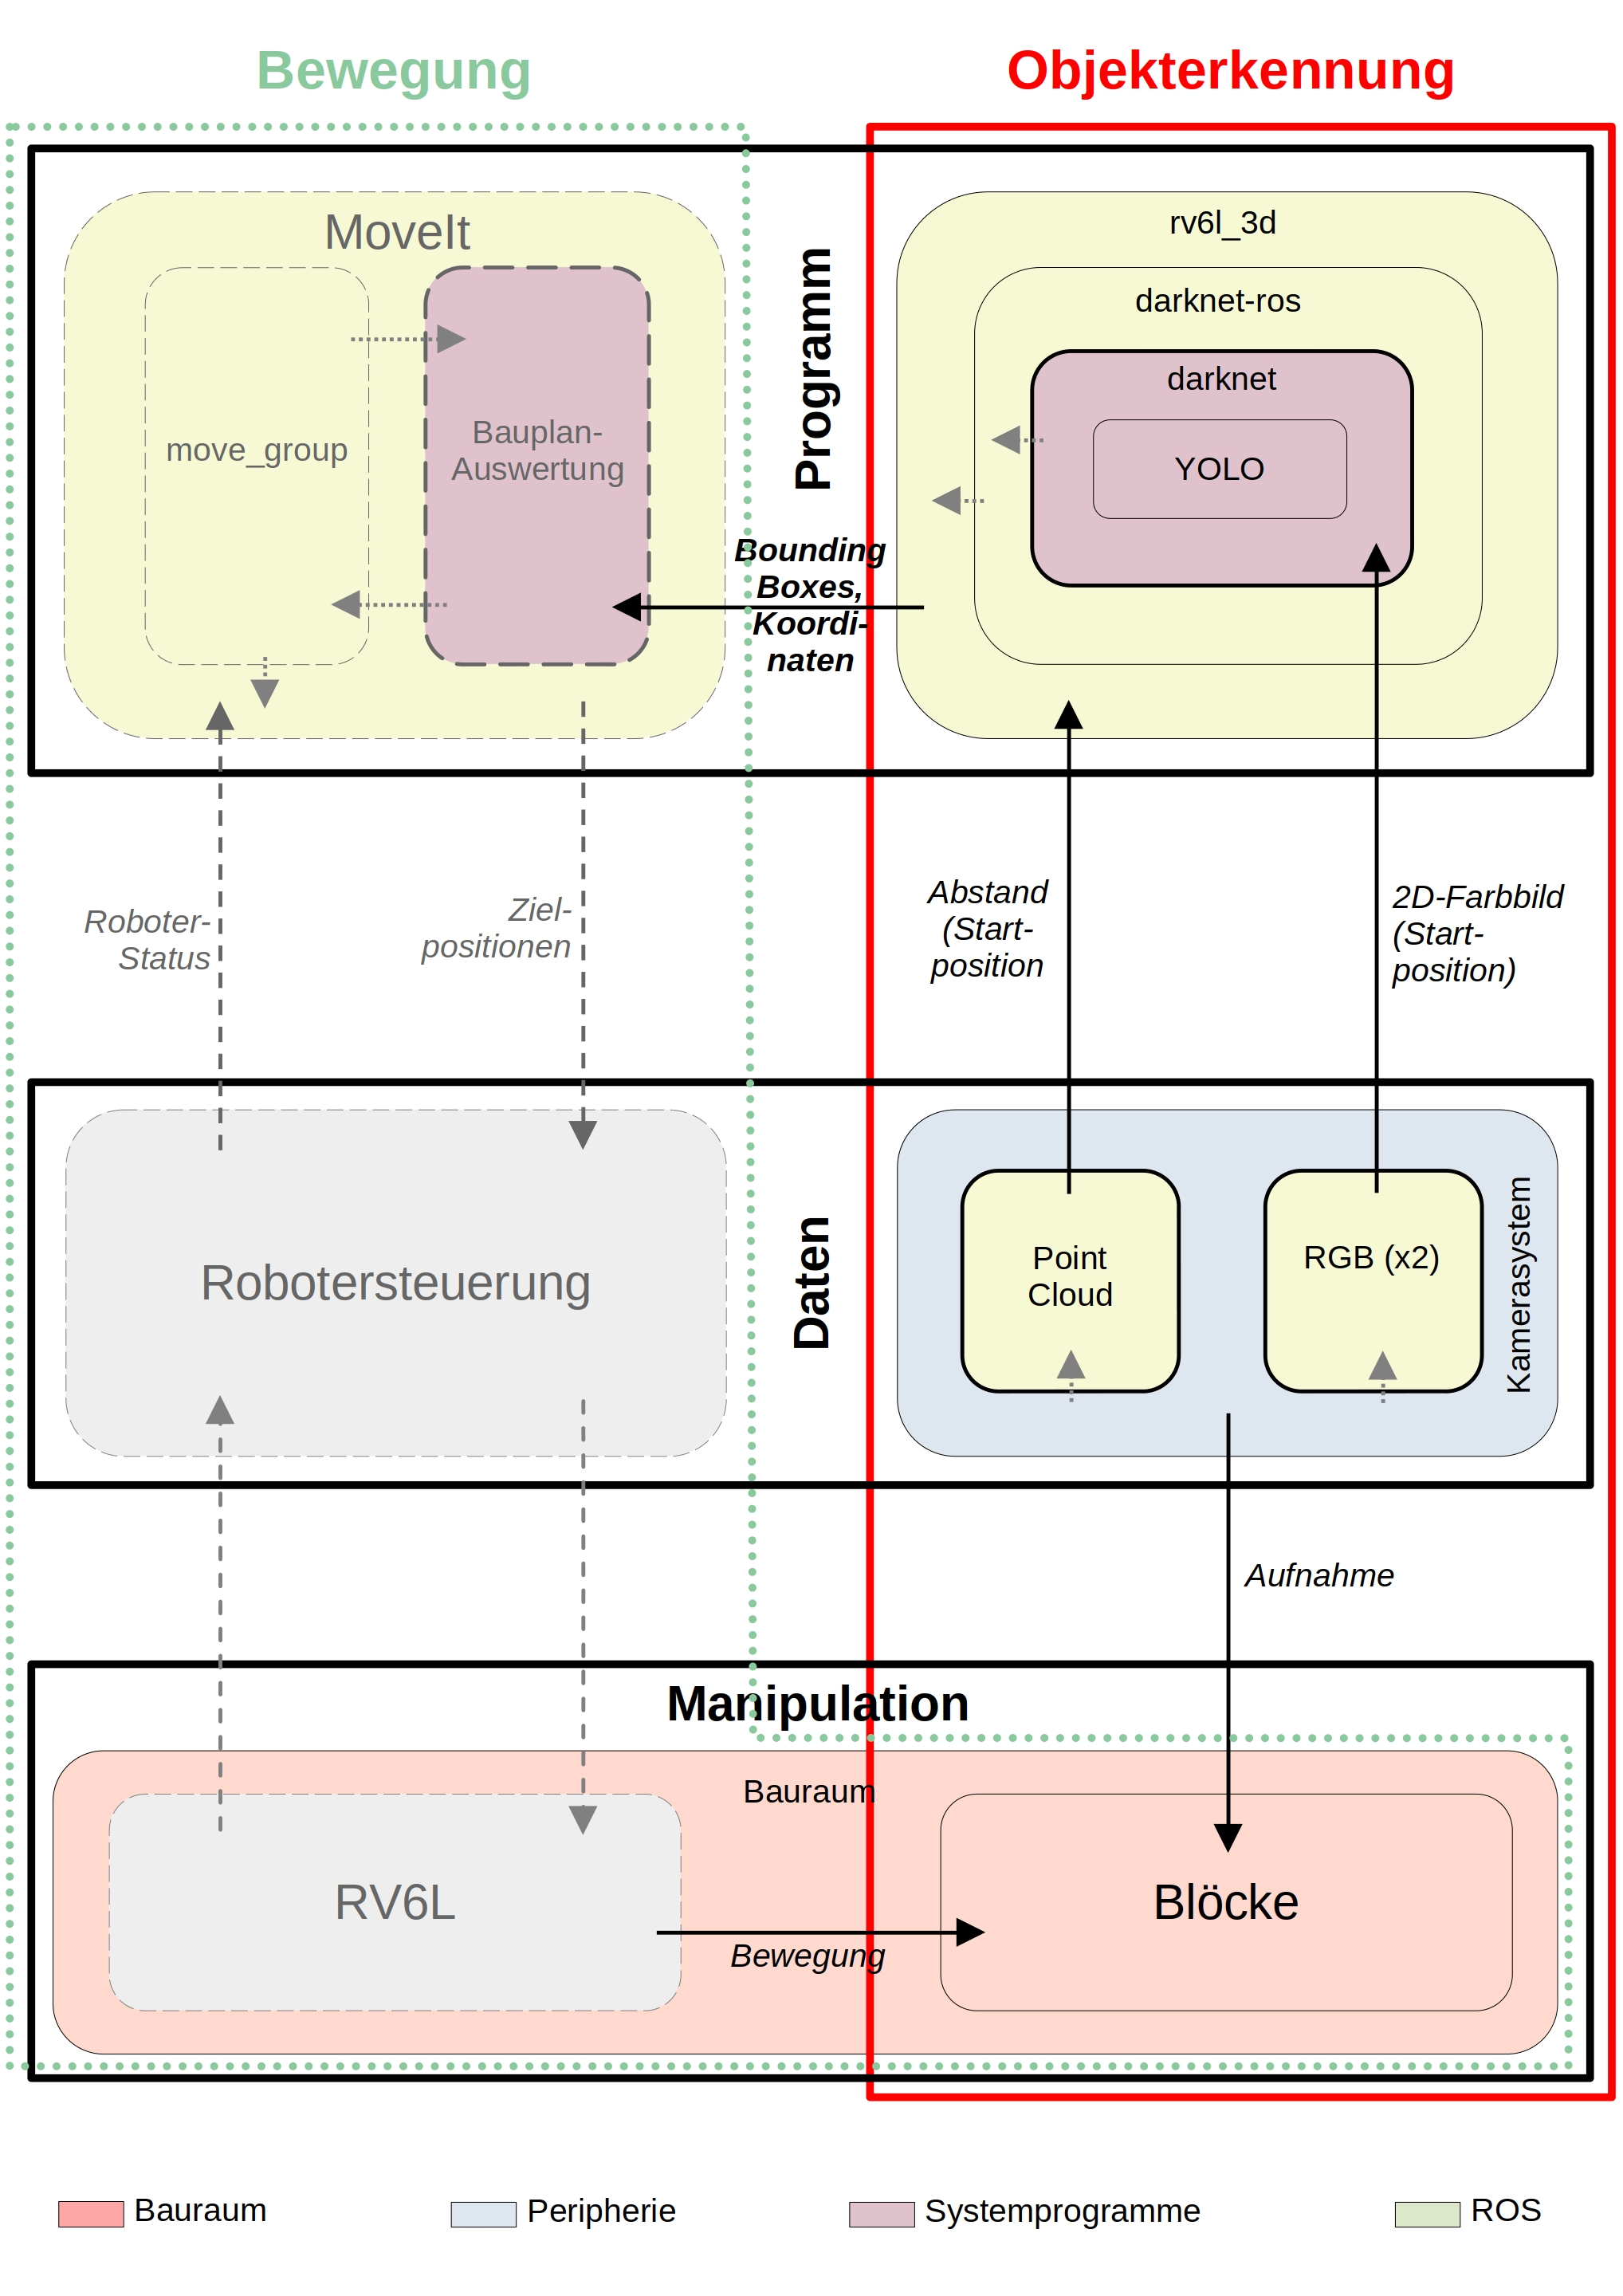
\includegraphics[width=\textwidth]{Bilder/gesamtsystem_struktur.jpg}
    \caption{Struktur des Gesamtsystems}
    \label{fig:gesamtsystem_struktur}
\end{figure}

Die Eingangsdaten des Systems bilden die Daten der beiden RGB-Kameras und der 3D-\textit{Point Cloud}. Diese nimmt mithilfe des RealSense-Treibers für \ac{ROS} ein Bild der Bauteile im Arbeitsbereich auf. Da es sich bei der RealSense um eine Stereokamera handelt, wird aus den Bildern beider Kameras mit Unterstützung der Punkte des Infrarotprojektors eine \textit{Point Cloud} berechnet, die anschließend vom \textit{rv6l\_3d}-Paket verwendet wird. Ein RGB-Bild der Kamera wird außerdem an das \textit{Darknet}-Framework und von dort an \textit{darknet\_ros} weitergegeben.

Die Grundlage der Erkennung bildet der \textit{\ac{YOLO}}-Algorithmus. Dieser wird vom \textit{Darknet}-Framework, was auch zum Training des Algorithmus verwendet wird, zur Erkennung der Objekte genutzt.  Es gibt die Objektklasse und jeweils die Koordinaten des oberen linken und unteren rechten Punktes der \textit{Bounding Boxes} zurück. Diese Koordinaten sind in Pixeln mit dem Mittelpunkt als Ursprung des 2D-Koordinatensystems angegeben. Für die Interaktion mit \ac{ROS} ist das Paket \textit{darknet\_ros} zuständig. Dieses nutzt einen \textit{Subscriber} zur Verwendung von Kameradaten und -aufnahmen und gibt relevante Daten an \textit{Darknet} weiter. Daraufhin extrahiert es relevante Informationen, die von \textit{Darknet} zurückgegeben werden. Unter Nutzung dieser Daten erfolgt eine Bereitstellung eigener \textit{Topics}, beispielsweise mit den Koordinaten der \textit{Bounding Boxes}, einer Visualisierung dieser und den Objektklassen.

Da die Position in Pixeln mit dem Abstand der Objekte variiert, werden für die Handhabung der Bauteile aufgrund der variablen Höhe und der wechselnden Kameraposition \textit{Bounding Box}-Koordinaten in einer abstandsunabhängigen Einheit benötigt. Dafür wird von dem in \refSec{subsec:rv6l_3d} erwähnten \textit{rv6l\_3d}-Paket unter Nutzung von Abstands- und Hardwareinformationen der 3D-Kamera und den \textit{Bounding Box}-Koordinaten eine Position in Metern relativ zum Kameramittelpunkt berechnet. Durch die Anpassung des Pakets auf den vorliegenden Anwendungsfall erfolgt keine Rückgabe der gesamten \textit{Bounding Box}, sondern der dreidimensionalen Position des Mittelpunktes der Objektoberfläche relativ zum Ursprung des Kamerakoordinatensystems. Dazu werden die Informationen aus dem \textit{darknet\_ros}-Paket mit den \textit{Point Cloud}-Daten des verwendeten Kamerasystems abgeglichen.

\section{Programmablauf}
Dieser Abschnitt beschreibt die Abläufe beim Start des Gesamtprogramms.

\begin{description}
    \item[1: Hardware-Interface] Zuerst werden die Programme für die Kommunikation zwischen \ac{ROS} und der Robotersteuerung und für die Interaktion mit dem realen Roboter gestartet.
    \item[2: Bilderkennung] Der für die Objektklassifikation und Positionserkennung zuständige \textit{Node} wird gestartet
    \item[3: Bewegungsalgorithmus] Zuletzt wird der Bewegungsalgorithmus gestartet. Dieser nutzt die Daten der Bilderkennung zur Berechnung der Objektpositionen und zum anschließenden Anordnen der Objekte nach dem vorgegebenen Bauplan.
\end{description}

\section{Bewegungsablauf}

\refFig{fig:gesamtsystem_ablauf} zeigt den Ablauf der gesamten Roboterbewegung nach Programmstart. Dieser kann in folgende Schritte unterteilt werden:

\begin{description}
    \item[1: Startposition] \beh Die Startposition kann beliebig gewählt werden, solange es sich nicht um eine singuläre Pose handelt.
    \item[2: Position für die Bilderkennung] Diese Position mit einer Höhe von $0,60m$ über der Tischebene stellt einen Kompromiss zwischen Zuverlässigkeit der Bilderkennung und Abdeckung des Arbeitsraumes, in dem sich die zufällig angeordneten Objekte befinden, dar. Diese Position kann je nach Anwendung individuell gewählt werden und hängt vom verwendeten Algorithmus, dem Datensatz zum Einlernen des Algorithmus, der Auflösung der Kamera und der Anzahl der Objekte ab.
    \item[3: 2D-Lokalisierung] Dieser Schritt ist notwendig, damit das System die Anzahl und Klasse der verwendeten Teile sowie eine ungefähre Position aller Objekte erfassen kann. Der in \refSec{subsec:intel_realsense} erwähnte Distanzbereich ist hier irrelevant, da nur die Position in horizontaler Ebene benötigt wird.
    \item[4: Teilmittelpunktposition] \beh Hier wird mithilfe des in Schritt 3 erkannten Mittelpunktes des ersten Objekts eine genauere Mittelpunktposition ausfindig gemacht.
    \item[5: 3D-Lokalisierung] Für die Lokalisierung wird das in \refSec{subsec:rv6l_3d} beschriebene Paket verwendet. Sobald sich die Kamera näherungsweise über dem Objektmittelpunkt befindet, wird der Abstand zwischen Kamera und dem durch eine \textit{Point Cloud} erkannten höchsten Punkt des Objekts ermittelt. Dieser Punkt wird in Form einer Liste aus vier Variablen mit Relativposition zur Kamera und Objektklasse zurückgegeben.
    \item[6: Zielposition] \beh Die im Bauplan festgelegte Zielposition des Teils wird angefahren.
    \item[7: Endposition] Nach Ablegen aller Teile kann der Roboter in eine beliebige, nicht singuläre Pose fahren.
\end{description}

Die Schritte \textbf{4} bis \textbf{6} werden für jedes Teil wiederholt.

\begin{figure}[ht]
    \centering
    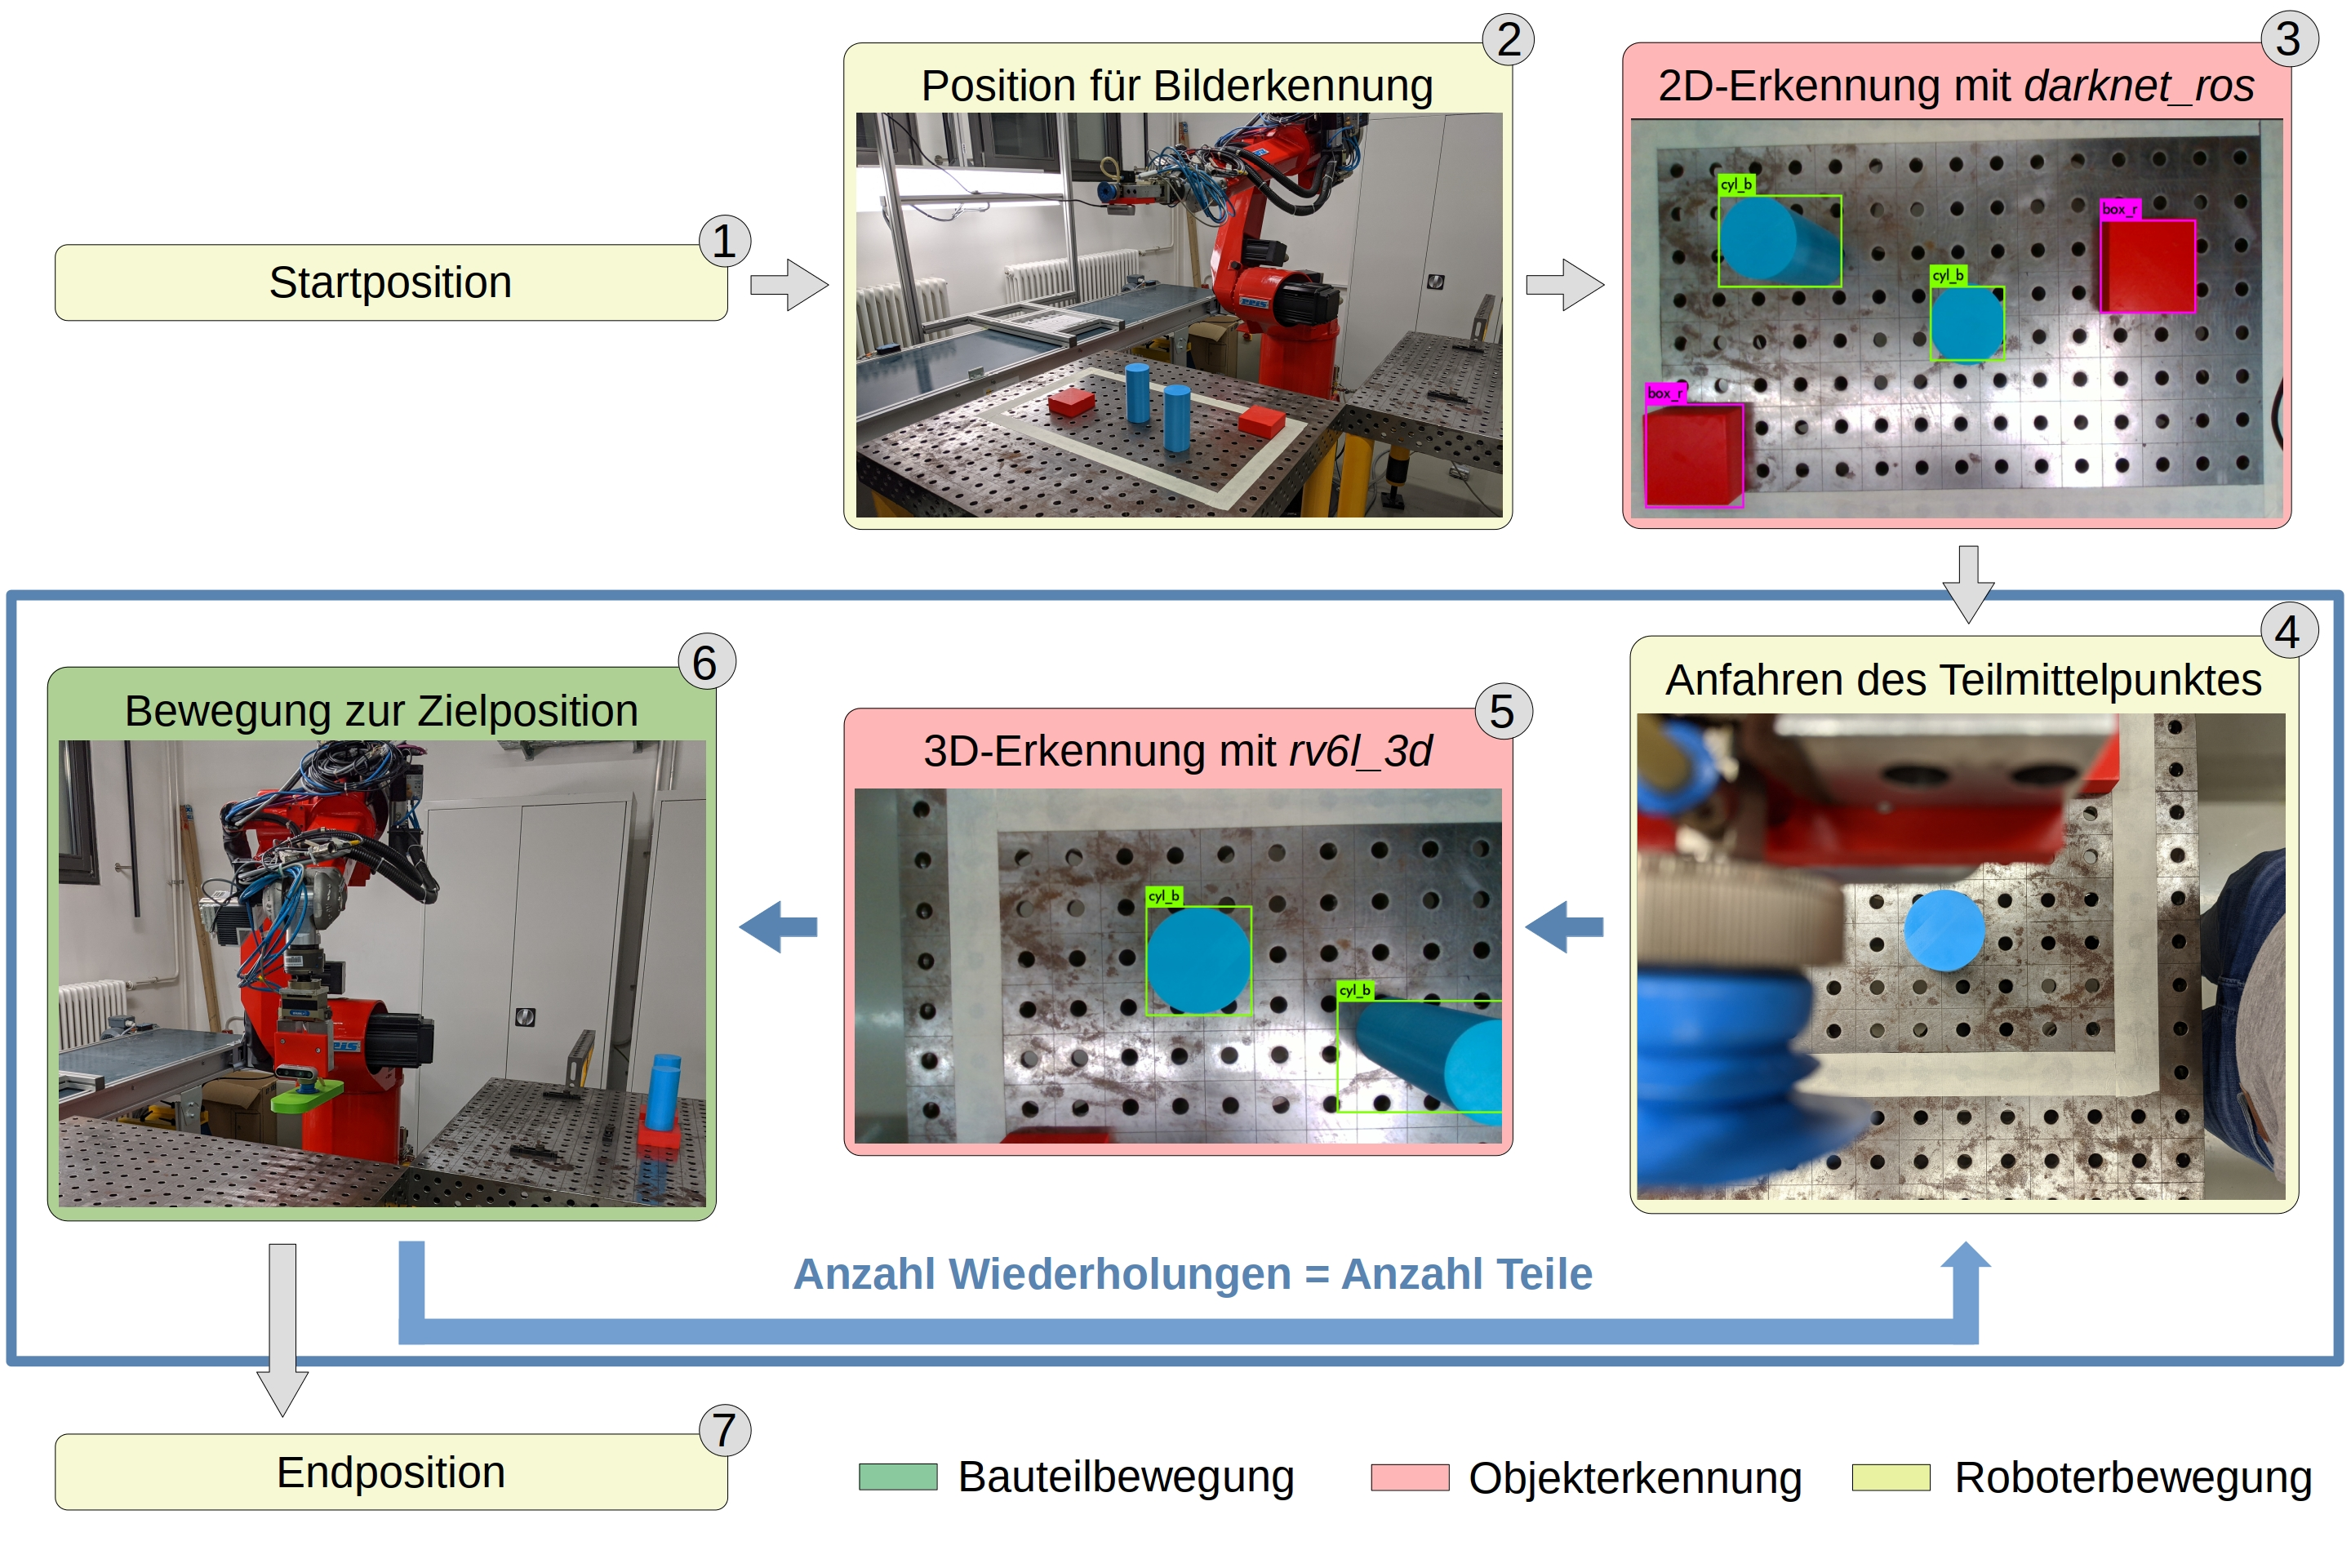
\includegraphics[angle=90, width=12cm]{Bilder/gesamtsystem_ablauf.jpg}
    \caption{Ablauf des Gesamtprogramms}
    \label{fig:gesamtsystem_ablauf}
\end{figure}
   \chapter{Evaluierung und Weiterentwicklung} \label{sec:evaluierung}

Folgendes Kapitel beinhaltet eine Evaluierung der verwendeten Methoden, Probleme und mögliche Optimierungsansätze in Bezug zur Objekterkennung. Verbesserungen der Handhabung sind in der Arbeit von Steinbeck aufgeführt \cite[Abschnitt~5]{steinbeck_entwicklung_2022}.

\section{Auswertung und Optimierung}

Die Verwendung von \textit{\ac{DL}} mit dem \textit{YOLOv3 Tiny}-Algorithmus ist aufgrund der für ein \textit{\ac{CNN}} sehr schnellen Klassifizierung und Positionserkennung auch mit schwacher Hardware und der ausreichenden Genauigkeit gut für die Anwendung geeignet. Auch die sehr geringe Fehlerrate trotz des kleinen Datensatzes zum Einlernen mit \textit{Darknet} spricht für \textit{\ac{DL}} und gegen die mit höherem Aufwand verbundenen Verwendung traditioneller \textit{\ac{CV}}. \textit{YOLO} kann außerdem mit dem Paket \textit{darknet\_ros}, für das schon Versionen für die Verwendung von \ac{ROS}-II verfügbar sind, gut in \ac{ROS} integriert werden. Aufgrund dieser Verfügbarkeit und der aktiven Entwicklung ist eine zukünftige Weiterentwicklung des \textit{rv6l\_3d}-Pakets gut umsetzbar. Wegen der Verfügbarkeit von \textit{Packages} wie \textit{darknet\_ros\_3d} ist die Verwendung der \ac{ROS}-Version \textit{Noetic} aktuell für die Anwendung geeignet. Mit der Nutzung der Intel RealSense als Alternative zur Microsoft Kinect kann aufgrund der Möglichkeit einer Befestigung am Endeffektor bei guter Ausrichtung dieser eine hohe Genauigkeit durch Ausgleichen der Positionsabweichung des verwendeten Roboters erzielt werden. Die Objekte können wegen der guten Kalibrierung ab Werk und des integrierten Infrarotprojektors sehr genau lokalisiert werden. Auch die Treiberunterstützung bietet mit Bereitstellung der Daten in \textit{OpenNI} kompatiblem Format Vorteile gegenüber anderen 3D-Kamerasystemen. Durch die zweistufige Mittelpunkterkennung kann der Zielpunkt sehr genau angefahren werden. Die Abweichung in $z$-Richtung ist hier minimal. Wegen Toleranzen bei der Befestigung der Kamera am Endeffektor können beispielsweise aufgrund einer Neigung Abweichungen in der $x$-$y$-Ebene entstehen. In den durchgeführten Tests waren diese allerdings gering und führten somit nicht zu Problemen. Die Kommunikation zwischen allen verwendeten \textit{Packages} funktioniert auch bei Nutzung verschiedener Programmiersprachen problemlos.

Auch wenn die Erkennungsrate durch den \textit{\ac{YOLO}}-Algorithmus bei den verwendeten Objekten sehr hoch ist, können vor allem bei ähnlichen Teilen Fehler bei der Klassifizierung auftreten. Mit der Verwendung eines größeren Datensatzes, einer Erhöhung von Auflösung oder Iterationen, oder Optimierungen des bestehenden Datensatzes kann die Erkennungsrate und Positionsgenauigkeit gesteigert werden. Die um $90$° gegenüber dem Endeffektor rotierte Montage ist aufgrund der Nähe zu einer Singularität des RV6L durch einen gestreckten Arm, bei dem die Achsen $4$ und $6$ deckungsgleich sind, in der maximalen Höhe limitiert. Eine Montage mit Blickrichtung parallel zum Kontaktpunkt des verwendeten Endeffektors würde diese Problematik lösen, jedoch den für die Kamera erreichbaren Bereich in $x$-Richtung des Basiskoordinatensystems verkleinern. Zur Optimierung der Genauigkeit in der $x$-$y$-Ebene kann eine Hand-Auge-Kalibrierung durchgeführt werden. Die Genauigkeit in $z$-Richtung wird auch hier nur wenig durch den Kamerawinkel beeinflusst.

\section{Ansätze zur Weiterentwicklung des rv6l\_3d-Pakets}

Während die Grundfunktionalität zur Objekterkennung und Positionserkennung gegeben ist, ist eine Weiterentwicklung des \textit{rv6l\_3d} Pakets notwendig. Aktuell funktioniert die Schnittstelle zwischen den Objekterkennungs- und Handhabungspaketen nur teilweise, da der \textit{Bounding Box Subscriber} \seeAtt{sec:handhabung} trotz Erkennung aller Bauteile nur die Position des zuletzt erkannten Blocks an das Programm zur Handhabung weitergibt. Somit wird eine Logik zur gleichzeitigen Weitergabe aller ungefähren Positionen der ersten Scanposition benötigt. Außerdem ist für die zweite Position eine Logik notwendig, die bei mehreren Teilen im Erkennungsbereich das mittlere Objekt identifiziert und nur dessen Position an den \textit{Subscriber} weitergibt. Somit ist die Erkennung und Aufnahme des korrekten Objekts gewährleistet. 
Zur Optimierung des Systems können außerdem folgende Ansätze genutzt werden: Aktuell ist der Erkennungsbereich durch den maximalen Aufnahmebereich des Kamerasystems limitiert, da der erste Scanvorgang des kompletten Bereichs nur mit fester Kameraposition durchgeführt wird. Dieses Problem kann durch die Implementierung einer Bewegung parallel zur $x$-$y$-Ebene des Basiskoordinatensystems während des Scans und anschließender Umrechnung der Objektpositionen in vom Handhabungsprogramm nutzbare Werte gelöst werden, wobei jedoch die durch die Perspektive abweichende Mittelpunktposition der Objekte beachtet werden muss. Auch eine Erkennung aus unterschiedlichen Kameraorientierungen oder ein von der Objektgröße abhängiger Abstand zwischen Kamera und Bauteil ist denkbar. Bei entsprechender Leistung des zur Bilderkennung verwendeten Computers ist ein Anfahren des Objekts mit Abgleich zwischen Kamera- und Objektmittelpunkt in Echtzeit zur Steigerung der Genauigkeit in $x$-$y$-Ebene möglich. Auch wenn der Mittelpunkt bei den verwendeten Objekten eine sinnvolle Greifposition darstellt, ist dieser nicht in allen Anwendungsfällen optimal. Eine Alternative ist etwa die Erkennung des höchsten Punktes eines Objekts oder einer geraden Fläche. Zur Verringerung der Fehleranfälligkeit kann zudem die Ablagehöhe für das Bauteil in der Zielposition gemessen werden, um Kollisionen mit Objekten im Ablagebereich zu vermeiden. Ein weiterer wichtiger Aspekt ist die Implementierung von Funktionen zur Ausnahmebehandlung. Wird beispielsweise ein Block nicht erkannt, kommt es beim Bewegungsprogramm in der aktuellen Form zu einem Fehler. Ein möglicher Lösungsansatz ist hier die Nutzung der 3D-\textit{Point Cloud}, um durch Erhöhungen im Bauraum Objekte zu erkennen und einen erneuten Scanvorgang zu starten. Auch die Erkennung von mehr Teilen, als im Bauplan genutzt werden, kann zu unvorhersehbaren Ereignissen beim Ausführen des Paktes führen.

Ein Nachteil des \textit{\ac{YOLO}}-Algorithmus ist die fehlende Unterstützung für \textit{\ac{OBBs}}. Stattdessen werden \textit{\ac{HBBs}} verwendet, die immer aus horizontalen und vertikalen Kanten ohne eine Möglichkeit zur Orientierungserkennung bestehen. Somit muss für eine Erkennung der Bauteilorientierung ein anderer Algorithmus genutzt werden. Dazu kann beispielsweise der Ansatz von Yin et al. zur Kalkulation von \textit{\ac{OBBs}} basierend auf \textit{\ac{YOLO}} genutzt werden \seeFig{fig:yolo_hbb_obb} \cite{yin_fast_2018}.

\begin{figure}[ht]
    \centering
    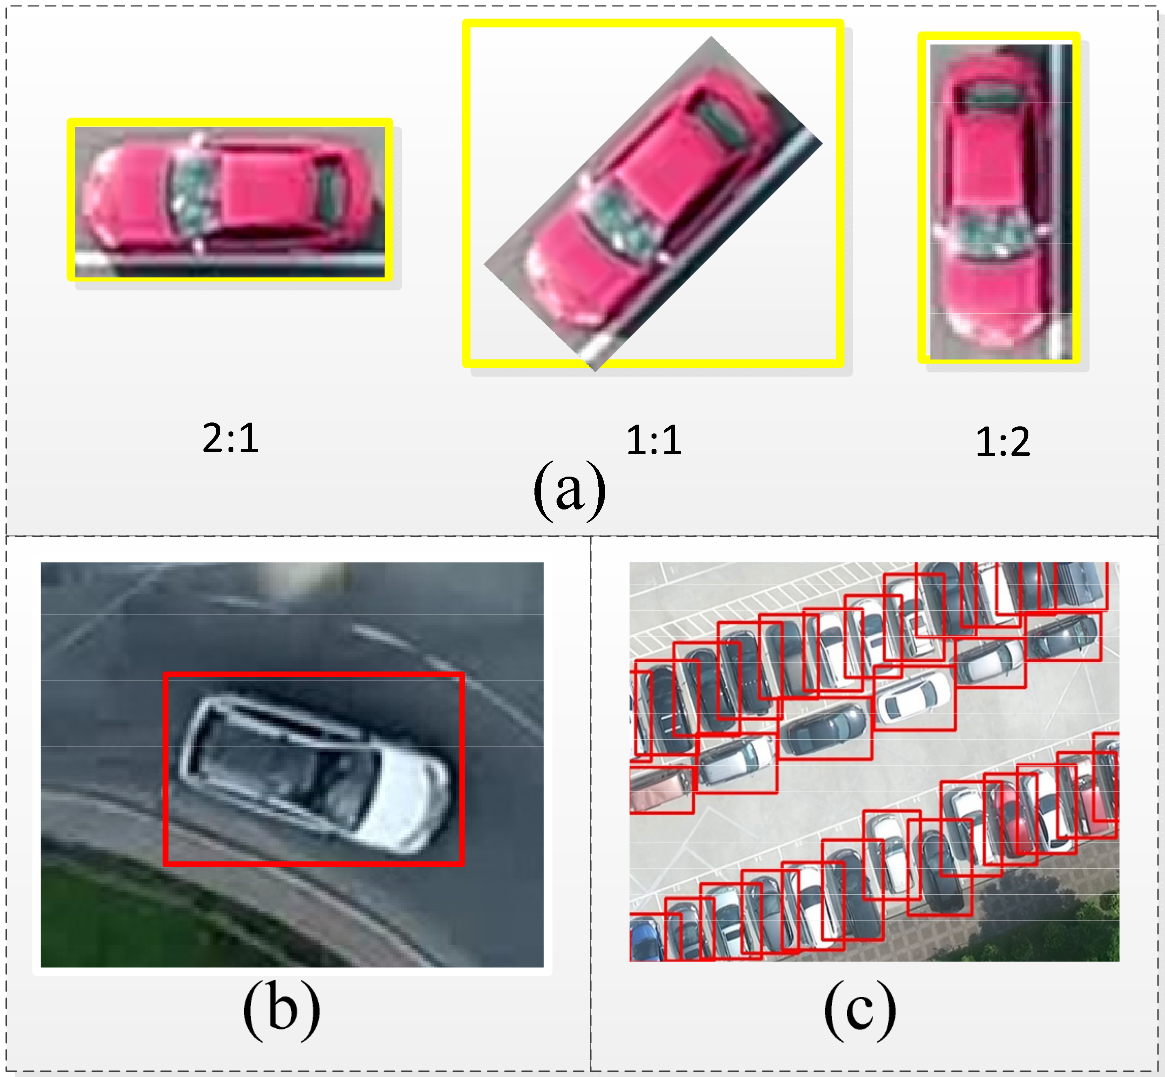
\includegraphics[height=6.29cm]{Bilder/yolo_hbb.png}
    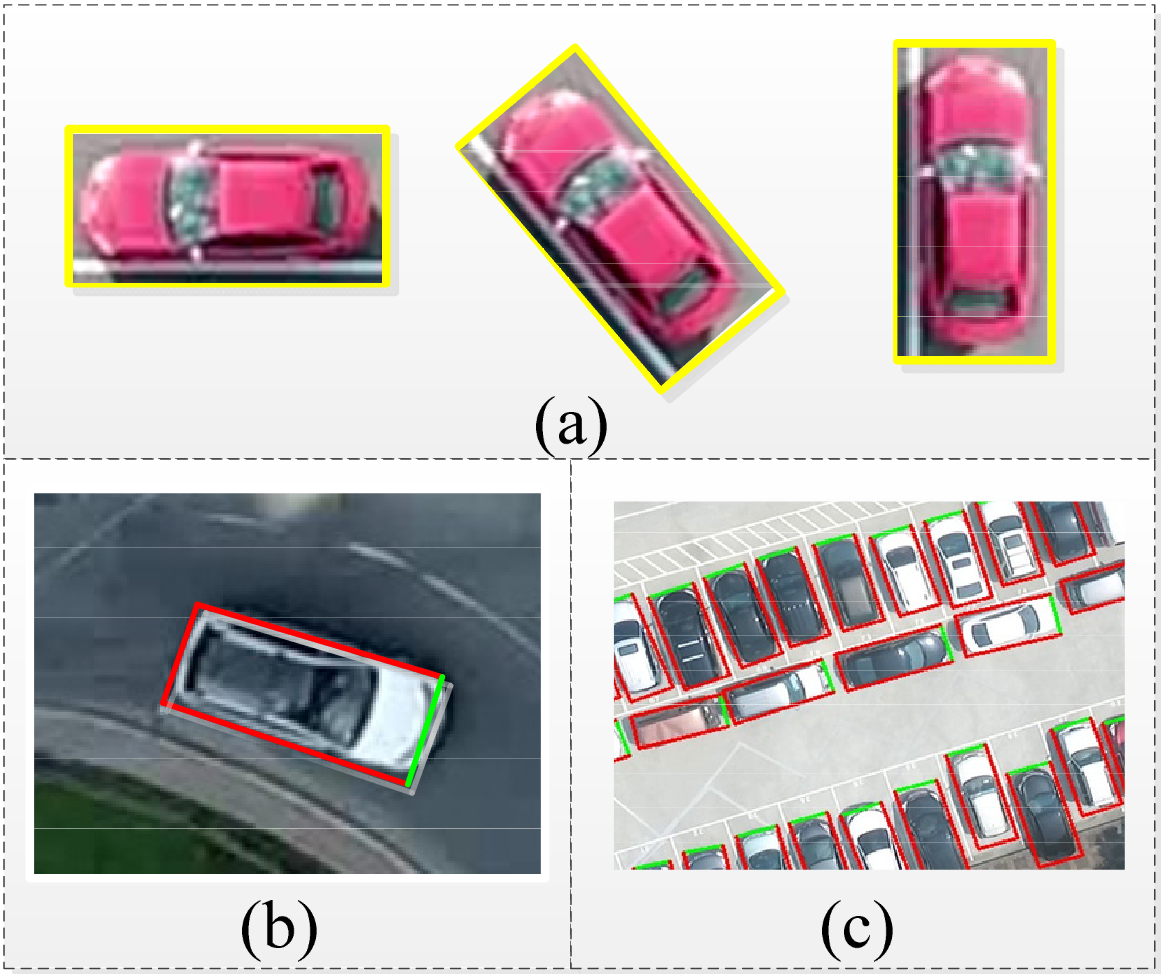
\includegraphics[height=6.29cm]{Bilder/yolo_obb.png}
    \caption{Vergleich zwischen HBBs (links) und OBBs (rechts) \cite{yin_fast_2018}}
    \label{fig:yolo_hbb_obb}
\end{figure}

Eine Implementierung von \textit{YOLOv5} mit \textit{\ac{OBBs}}, die ein Paket für die Nutzung mit \ac{ROS} beinhaltet, wurde im Dezember 2021 unter dem Namen "RoSA: Cube Detector" veröffentlicht \cite{hempel_rosa_2021}.

Eine weitere Optimierung besteht in der Kollisionsvermeidung mit erkannten Objekten. Der genutzte Bahnplanungsalgorithmus umfährt bekannte Objekte im Bauraum. Jedoch werden die erkannten Bauteile diesem nicht zur Verfügung gestellt. Die Bereitstellung der Kollisionsobjekte kann entweder über Einfügen der bekannten Objekte an den durch die Objekterkennung ermittelten Mittelpunktpositionen in die Simulation oder der Nutzung der von der Kamera generierten \textit{Point Cloud} umgesetzt werden.
   \chapter{Fazit}

Die Nutzung von 3D-Kamerasystemen und \textit{\acp{CNN}} in Verbindung mit Robotern schafft eine gute Grundlage für die Handhabung verschiedener Teile. An den Ergebnissen werden der Fortschritt und die Möglichkeiten aktueller neuronaler Netzte wie \textit{\ac{YOLO}}, die auch mit vergleichsweise schwacher Hardware geboten werden, deutlich. Durch die Nutzung des \ac{ROS} ist eine standardisierte Schnittstelle für die Kommunikation verschiedener Pakete verfügbar. Hier erschließen sich die Vorteile der Open-Source-Software besonders. Die Verwendung bestehender Pakete als Grundlage für die Implementierung der Objekterkennung unter Nutzung des Meta-Betriebssystems schafft eine gute Basis für die Umsetzung der Bilderkennung. 

Das Ziel der Erkennung von Klasse und Position einer ungeordneten Zusammenstellung von Objekten wurde erreicht. Das auf \textit{darknet\_ros\_3d} basierende \textit{rv6l\_3d} kann mithilfe des \ac{ROS} und eines 3D-Kamerasystems zuverlässig einzelne Bauteile im Aufnahmebereich erkennen und Positionsdaten und Art an den \textit{Subscriber} des Handhabungsprogramms weitergeben. Die Intel RealSense 435 eignet sich durch die kleine Baugröße, genaue Abstandsberechnung und für den Anwendungsfall ausreichende Auflösung der Kameras gut für die durch \textit{rv6l\_3d} umgesetzte Positionserkennung. Ein Nachteil der genutzten Konfiguration ist die Nähe zu einer singulären Stellung in der Scanposition. Eine Befestigung des Kamerasystems parallel zum Endeffektor kann diesen lösen, was allerdings eine Verringerung des Erkennungsbereichs zur Folge hat. Die Nutzung von \textit{\ac{DL}} zur Erkennung der Objekte bietet im Vergleich zu traditioneller \textit{\ac{CV}} viele Vorteile, wie die hohe Erkennungsrate oder den vergleichsweise wenig komplexen Prozess zur Erstellung eigener Datensätze. So eignet sich \textit{\ac{YOLO}} in den Grundzügen wegen der für ein \textit{\ac{CNN}} guten Performance und kontinuierlich zuverlässigen Erkennung der verwendeten Objekte sehr gut für den Anwendungsfall.

Auch wenn eine Grundfunktionalität gegeben ist, muss das \textit{rv6l\_3d}-Paket im Hinblick auf die in \refSec{sec:evaluierung} beschriebenen Probleme optimiert werden. Neben notwendigen Verbesserungen wie der Weitergabe mehrerer Bauteile durch die Schnittstelle zwischen Objekterkennungs- und Handhabungsprogramm und der Ausnahmebehandlung können die erwähnten Vorschläge wie die Positionserkennung zu einer Erweiterung des Anwendungsbereichs genutzt werden.

Die Ergebnisse zeigen die durch \ac{ROS} gebotenen Möglichkeiten zur Kombination verschiedener Hardware und Software. Dies wird besonders in der Übersicht des Gesamtsystems \seeFig{fig:gesamtsystem_struktur} deutlich. Durch diese Eigenschaft bietet das System eine Basis, die für zukünftige Weiterentwicklungen genutzt werden kann.

   \backmatter
   \pagenumbering{Roman}
   \setcounter{page}{4}

   \newpage
   \addtotoc{Abbildungsverzeichnis}
   \listoffigures
   \begin{flushleft}
   \addtotoc{Literatur}
   \printbibliography  % Bibliographie erzeugen
   \end{flushleft}
   \appendix
   \renewcommand{\thesection}{\Alph{section}}
   \part*{Anhang}
%\chapter{Anhang}
\appendixtoc

\vspace*{\fill}
Auf dem beigelegten Datenträger (Verzeichnis \lstinline{David Gries/Dokumente und Medien}) befindet sich eine HTML-Datei mit Anleitungen zur Installation der \ac{ROS}-Pakete. Außerdem ist der vollständige Quellcode aller relevanten Pakete und eine Demonstration des Projekts in Form eines Videos enthalten. Entfernte Zeilen zur Verbesserung der Übersicht sind mit \lstinline{[ . . . ]} gekennzeichnet. Die Verzeichnisstruktur von Quellcode und Konfigurationsdateien richtet sich dabei nach der Struktur des folgenden schriftlichen Anhangs. Dieser beinhaltet alle Code-Abschnitte, die zum besseren Verständnis der Arbeit beitragen.

Informationen zu Lizenzen der in dieser Arbeit verwendeten Projekte sind auf dem Datenträger zu finden. Diese befinden je nach Anforderungen der jeweiligen Lizenz im Ordner des Softwarepakets oder am Anfang des Quellcodes. Kennzeichnungspflichtige Änderungen wurden an den entsprechenden Stellen ergänzt.

\newpage
\overfullrule=0pt\dirtree{%
  .1 David Gries.
  .2 Anhang A - RV6L 3D.
  .3 A\_1 - Konfiguration.
  .4 RV6L.yaml.
  .4 ros.yaml.
  .4 darknet\_3d.yaml.
  .3 A\_2 - Bounding Box Funktion.
  .4 Darknet3DListener.cpp.
  .4 Darknet3D.cpp.
  .4 darknet3d\_node.cpp.
  .3 A\_3 - Bounding Box Message.
  .4 RV6L\_positions.msg.
  .4 RV6L\_position.msg.
  .3 A\_4 - Launchfiles.
  .4 first.launch.
  .4 RV6L.launch.
  .4 second.launch.
  .3 A\_5 - ROS Package.
  .4 package.xml.
  .2 Anhang B - RealSense Launchfile.
  .3 RV6L.launch.
  .2 Anhang C - Handhabung.
  .3 C\_1 - Bounding Box Subscriber.
  .4 subscriber\_cam.py.
  .3 C\_2 - Anfahren des Objekts.
  .4 pick\_and\_place\_detection.py.
  .2 Anhang D - Darknet.
  .3 D\_1 - Darknet Konfiguration.
  .4 RV6L.cfg.
  .3 D\_2 - Objekt Konfiguration.
  .4 obj.data.
  .3 D\_3 - Generator fuer train.
  .4 generate\_train.py.
  .2 Dokumente und Medien.
  .3 Bachelorarbeit David Gries.pdf.
  .3 Bilder und Quelldateien/....
  .3 Installationsanleitung.html.
  .3 Objekterkennung Demo.mp4.
}

%├── Anhang A - RV6L 3D
%│   ├── A_1 - Konfiguration
%│   │   ├── darknet_3d.yaml
%│   │   ├── ros.yaml
%│   │   └── RV6L.yaml
%│   ├── A_2 - Bounding Box Funktion
%│   │   ├── Darknet3D.cpp
%│   │   ├── Darknet3DListener.cpp
%│   │   └── darknet3d_node.cpp
%│   ├── A_3 - Bounding Box Message
%│   │   ├── RV6L_position.msg
%│   │   └── RV6L_positions.msg
%│   ├── A_4 - Launchfiles
%│   │   ├── first.launch
%│   │   ├── RV6L.launch
%│   │   └── second.launch
%│   └── A_5 - ROS Package
%│       └── package.xml
%├── Anhang B - RealSense Launchfile
%│   └── RV6L.launch
%├── Anhang C - Handhabung
%│   ├── C_1 - Bounding Box Subscriber
%│   │   └── subscriber_cam.py
%│   └── C_2 - Anfahren des Objekts
%│       └── pick_and_place_detection.py
%├── Anhang D - Darknet
%│   ├── D_1 - Darknet Konfiguration
%│   │   └── RV6L.cfg
%│   ├── D_2 - Objekt Konfiguration
%│   │   └── obj.data
%│   └── D_3 - Generator fuer train
%│       └── generate_train.py
%└── Dokumente und Medien
%    ├── Installationsanleitung.html
%    └── Objekterkennung Demo.mp4

\newpage\section{RV6L 3D} \label{sec:rv6l_3d}

\subsection{Konfiguration} \label{subsec:bounding_config}

\subsubsection{Hauptkonfiguration}

\lstinline{[darknet_3d.yaml]}

\begin{lstlisting}
darknet_ros_topic: /darknet_ros/bounding_boxes
output_bbx3d_topic: /darknet_ros_3d/bounding_boxes
point_cloud_topic: /camera/depth_registered/points
working_frame: camera_link
mininum_detection_thereshold: 0.3
minimum_probability: 0.3
interested_classes: ["box_r", "box_g", "cyl_b"]
\end{lstlisting}


\subsubsection{Darknet ROS Konfiguration} \label{subsec:darknet_rosconfig}

\lstinline{[ros.yaml]}

\begin{lstlisting}
subscribers:

  camera_reading:
    topic: /camera/color/image_raw
    queue_size: 1
[ . . . ]
\end{lstlisting}

\subsubsection{RV6L Konfiguration} \label{subsec:darknet_rv6lconfig}

\lstinline{[rv6l.yaml]}

\begin{lstlisting}
yolo_model:

  config_file:
    name: RV6L.cfg
  weight_file:
    name: RV6L.weights
  threshold:
    value: 0.3
  detection_classes:
    names:
      - box_r
      - box_g
      - cyl_b
\end{lstlisting}

\subsection{Bounding Box Funktion} \label{subsec:bounding_funkt}

\lstinline{[darknet3d_node.cpp, Darknet3D.cpp, Darknet3DListener.cpp]}

\begin{lstlisting}[language=c++]
[ . . . ]

void
Darknet3D::calculate_boxes(const sensor_msgs::PointCloud2& cloud_pc2,
    const pcl::PointCloud<pcl::PointXYZRGB>::ConstPtr cloud_pcl,
    rv6l_3d_msgs::RV6L_positions* boxes) // Funktion zur Berechnung der Positionsdaten
{
  boxes->header.stamp = cloud_pc2.header.stamp;
  boxes->header.frame_id = working_frame_;

  for (auto bbx : original_bboxes_)
  {
    if ((bbx.probability < minimum_probability_) ||
        (std::find(interested_classes_.begin(), interested_classes_.end(), bbx.Class) == interested_classes_.end()))
    {
      continue;
    }

    int center_x, center_y;

    center_x = (bbx.xmax + bbx.xmin) / 2;
    center_y = (bbx.ymax + bbx.ymin) / 2;
    
    int pcl_index = (center_y* cloud_pc2.width) + center_x;
    pcl::PointXYZRGB center_point =  cloud_pcl->at(pcl_index);
    
    if (std::isnan(center_point.x))
      continue;
    
    float maxx, minx, maxy, miny, maxz, minz, midx, midy, midz, w, h, d;
    
    maxx = maxy = maxz =  -std::numeric_limits<float>::max();
    minx = miny = minz =  std::numeric_limits<float>::max();
  
    for (int i = bbx.xmin; i < bbx.xmax; i++)
      for (int j = bbx.ymin; j < bbx.ymax; j++)
      {
        pcl_index = (j* cloud_pc2.width) + i;
        pcl::PointXYZRGB point =  cloud_pcl->at(pcl_index);
    
        if (std::isnan(point.x))
          continue;
    
        if (fabs(point.x - center_point.x) > mininum_detection_thereshold_)
              continue;
    
        maxx = std::max(point.x, maxx); 
        maxy = std::max(point.y, maxy);
        maxz = std::max(point.z, maxz);
        minx = std::min(point.x, minx);
        miny = std::min(point.y, miny);
        minz = std::min(point.z, minz);

        midx = (maxx + minx) / 2; // Objektmittelpunkt (x)
        midy = (maxy + miny) / 2; // Objektmittelpunkt (y)
        midz = (maxz + minz) / 2; // Objektmittelpunkt (z)
      }
    
    rv6l_3d_msgs::RV6L_position bbx_msg;
    bbx_msg.Class = bbx.Class;
    bbx_msg.probability = bbx.probability;

    bbx_msg.w = midy; // "horizontale" Position
    bbx_msg.h = midz; // "vertikale" Position
    bbx_msg.d = minx; // Abstand (min)

    boxes->bounding_boxes.push_back(bbx_msg);
  }
}

[ . . . ]
\end{lstlisting}

\subsection{Bounding Box Message} \label{subsec:bounding_strukt}

\lstinline{[RV6L_position.msg, RV6L_positions.msg]}

\subsubsection{Struktur}

% Msg Struktur
\begin{lstlisting}
string Class
float32 probability
float32 w
float32 h
float32 d
\end{lstlisting}

\subsubsection{Ausgabe (Topic)} 
% Msg Ausgabe
\begin{lstlisting}[language=c]
---
 header: 
  seq: 5
  stamp: 
    secs: 1644414390
    nsecs: 296165943
  frame_id: "camera_link"
bounding_boxes: 
  - 
    Class: "box_r"                  // Objektklasse
    probability: 0.9995404481887817 // Wahrscheinlichkeit
    w: 0.3090042471885681           // hor. Position in m
    h: 0.18566249310970306          // ver. Position in m
    d: 0.5624291300773621           // Abstand in m
\end{lstlisting}

\subsection{Launchfiles} \label{subsec:bounding_launchfiles}

\subsubsection{RV6L 3D (Darknet)}

\lstinline{[RV6L.launch]}

\begin{lstlisting}[language=xml]
<launch>

  <!-- Config camera image topic  -->
  <arg name="camera_rgb_topic" default="/camera/color/image_raw" />

  <!-- Console launch prefix -->
  <arg name="launch_prefix" default=""/>

  <!-- Config and weights folder. -->
  <arg name="yolo_weights_path"          default="$(find darknet_ros)/yolo_network_config/weights"/>
  <arg name="yolo_config_path"           default="$(find darknet_ros)/yolo_network_config/cfg"/>

  <!-- ROS and network parameter files -->
  <arg name="ros_param_file"             default="$(find darknet_ros)/config/ros.yaml"/>
  <arg name="network_param_file"         default="$(find darknet_ros)/config/RV6L.yaml"/>

  <!-- Load parameters -->
  <rosparam command="load" ns="darknet_ros" file="$(arg network_param_file)"/>
  <rosparam command="load" file="$(find darknet_ros)/config/ros.yaml"/>
  <param name="darknet_ros/subscribers/camera_reading/topic" type="string" value="$(arg camera_rgb_topic)" />

  <!-- Start darknet and ros wrapper -->
  <node pkg="darknet_ros" type="darknet_ros" name="darknet_ros" output="screen" launch-prefix="$(arg launch_prefix)">

    <param name="weights_path"          value="$(arg yolo_weights_path)" />
    <param name="config_path"           value="$(arg yolo_config_path)" />
  </node>

  <!-- Start darknet ros 3d -->
  <node pkg="darknet_ros_3d" type="darknet3d_node" name="darknet_3d" output="screen">
    <rosparam command="load" file="$(find darknet_ros_3d)/config/darknet_3d.yaml" />
  </node>
</launch>
\end{lstlisting}

\subsubsection{rv6l\_object\_detection}

\lstinline{[first.launch]}

\begin{lstlisting}[language=xml]
  <launch>

  <!-- Start RealSense driver -->
  <include file="$(find realsense2_camera)/launch/RV6L.launch" />

  <!-- Start rv6l_3d -->
  <include file="$(find darknet_ros_3d)/launch/RV6L.launch" />
  
  <!-- Start hardware interface -->
  <include file="$(find rsv_cartesian_interface)/test/test_hardware_interface.launch" /> 

</launch>
\end{lstlisting}

\lstinline{[second.launch]}

\begin{lstlisting}[language=xml]
  <launch>

  <!-- Start execution -->
  <include file="$(find rv6l_cell_config)/launch/rv6l_moveit_planning_execution_tut.launch" />

  <!-- Start movement -->

</launch>
\end{lstlisting}

\subsection{ROS Package}

\lstinline{[package.xml]}

\begin{lstlisting}[language=xml]
<?xml version="1.0"?>
<package format="2">
  <name>rv6l_main</name>
  <version>1.0.0</version>
  <description>Object detection and Point Cloud mapping using ROS Noetic and Intel RealSense 435</description>
  
  <maintainer email="dgries@mailbox.org">David Gries</maintainer>
  
  <url type="website">https://rzlapgle01.intern.th-ab.de/s170417/rv6l-kinect</url>
  
  <buildtool_depend>catkin</buildtool_depend>
  
  <build_depend>realsense2_camera</build_depend>
  <build_depend>darknet_ros_3d</build_depend>
  <build_depend>rv6l_3d_msgs</build_depend>
  <build_depend>opencv_apps</build_depend>
  <build_depend>pcl_ros</build_depend>
  <build_depend>rv6l_pick_and_place</build_depend>
  <build_depend>forward_command_controller</build_depend>
  <build_depend>joint_state_controller</build_depend>
  <build_depend>joint_trajectory_controller</build_depend>
  <build_depend>position_controllers</build_depend>
  <build_depend>rqt_joint_trajectory_controller</build_depend>
  <build_depend>rsv_cartesian_interface</build_depend>
  <build_depend>rsv_joint_interface</build_depend>
  <build_depend>rv6l</build_depend>
  <build_depend>rv6l_cell</build_depend>
  <build_depend>rv6l_cell_config</build_depend>
  <build_depend>rv6l_config</build_depend>
  <build_depend>nlopt</build_depend>
  
  <build_export_depend>realsense2_camera</build_export_depend>
  <build_export_depend>darknet_ros_3d</build_export_depend>
  <build_export_depend>rv6l_3d_msgs</build_export_depend>
  <build_export_depend>opencv_apps</build_export_depend>
  <build_export_depend>pcl_ros</build_export_depend>
  <build_export_depend>rv6l_pick_and_place</build_export_depend>
  <build_export_depend>forward_command_controller</build_export_depend>
  <build_export_depend>joint_state_controller</build_export_depend>
  <build_export_depend>joint_trajectory_controller</build_export_depend>
  <build_export_depend>position_controllers</build_export_depend>
  <build_export_depend>rqt_joint_trajectory_controller</build_export_depend>
  <build_export_depend>rsv_cartesian_interface</build_export_depend>
  <build_export_depend>rsv_joint_interface</build_export_depend>
  <build_export_depend>rv6l</build_export_depend>
  <build_export_depend>rv6l_cell</build_export_depend>
  <build_export_depend>rv6l_cell_config</build_export_depend>
  <build_export_depend>rv6l_config</build_export_depend>
  <build_export_depend>nlopt</build_export_depend>
  
  <exec_depend>realsense2_camera</exec_depend>
  <exec_depend>darknet_ros_3d</exec_depend>
  <exec_depend>rv6l_3d_msgs</exec_depend>
  <exec_depend>opencv_apps</exec_depend>
  <exec_depend>pcl_ros</exec_depend>
  <exec_depend>rv6l_pick_and_place</exec_depend>
  <exec_depend>forward_command_controller</exec_depend>
  <exec_depend>joint_state_controller</exec_depend>
  <exec_depend>joint_trajectory_controller</exec_depend>
  <exec_depend>position_controllers</exec_depend>
  <exec_depend>rqt_joint_trajectory_controller</exec_depend>
  <exec_depend>rsv_cartesian_interface</exec_depend>
  <exec_depend>rsv_joint_interface</exec_depend>
  <exec_depend>rv6l</exec_depend>
  <exec_depend>rv6l_cell</exec_depend>
  <exec_depend>rv6l_cell_config</exec_depend>
  <exec_depend>rv6l_config</exec_depend>
  <exec_depend>nlopt</exec_depend>
  
  <export>
  </export>
</package>
\end{lstlisting}

\newpage\section{Realsense Launchfile} \label{sec:realsense}

\lstinline{[RV6L.launch]}

\begin{lstlisting}[language=xml]
<!--
A launch file, derived from rgbd_launch and customized for Realsense ROS driver,
to publish XYZRGB point cloud like an OpenNI camera.

NOTICE: To use this launch file you must first install ros package rgbd_launch.

To launch Realsense with software registeration (ROS Image Pipeline and rgbd_launch):
    $ roslaunch realsense2_camera rs_rgbd.launch
Processing enabled by ROS driver:
    # depth rectification
Processing enabled by this node:
    # rgb rectification
    # depth registeration
    # pointcloud_xyzrgb generation

To launch Realsense with hardware registeration (ROS Realsense depth alignment):
    $ roslaunch realsense2_camera rs_rgbd.launch align_depth:=true
Processing enabled by ROS driver:
    # depth rectification
    # depth registration
Processing enabled by this node:
    # rgb rectification
    # pointcloud_xyzrgb generation
-->

<launch>
  <arg name="camera"              default="camera"/>
  <arg name="tf_prefix"           default="$(arg camera)"/>
  <arg name="external_manager"    default="false"/>
  <arg name="manager"             default="realsense2_camera_manager"/>

  <!-- Camera device specific arguments -->

  [ . . . ]

  <arg name="depth_width"         default="-1"/>
  <arg name="depth_height"        default="-1"/>
  <arg name="enable_depth"        default="true"/>

  [ . . . ]

  <arg name="color_width"         default="-1"/>
  <arg name="color_height"        default="-1"/>
  <arg name="enable_color"        default="true"/>

  [ . . . ]

  <arg name="depth_fps"           default="-1"/>
  <arg name="infra_fps"           default="-1"/>
  <arg name="color_fps"           default="-1"/>

  [ . . . ]

  <arg name="enable_pointcloud"   default="false"/>
  <arg name="enable_sync"         default="true"/>
  <arg name="align_depth"         default="true"/>
  <arg name="filters"             default="pointcloud"/>

  <arg name="publish_tf"          default="true"/>
  <arg name="tf_publish_rate"     default="0"/> <!-- 0 - static transform -->

  <!-- rgbd_launch specific arguments -->

  <!-- Arguments for remapping all device namespaces -->
  <arg name="rgb"                             default="color" />
  [ . . . ]
  <arg name="depth"                           default="depth" />
  <arg name="depth_registered_pub"            default="depth_registered" />
  <arg name="depth_registered"                default="depth_registered" unless="$(arg align_depth)" />
  <arg name="depth_registered"                default="aligned_depth_to_color" if="$(arg align_depth)" />
  <arg name="depth_registered_filtered"       default="$(arg depth_registered)" />
  <arg name="projector"                       default="projector" />

  <!-- Processing Modules -->
  <arg name="rgb_processing"                  default="true"/>
  [ . . . ]
  <arg name="depth_processing"                default="false"/>
  <arg name="depth_registered_processing"     default="true"/>
  [ . . . ]

  <group ns="$(arg camera)">

    <!-- Launch the camera device nodelet-->
    <include file="$(find realsense2_camera)/launch/includes/nodelet.launch.xml">

      [ . . . ]

      <arg name="enable_pointcloud"        value="$(arg enable_pointcloud)"/>
      <arg name="enable_sync"              value="$(arg enable_sync)"/>
      <arg name="align_depth"              value="$(arg align_depth)"/>

      [ . . . ]

      <arg name="depth_width"              value="$(arg depth_width)"/>
      <arg name="depth_height"             value="$(arg depth_height)"/>
      <arg name="enable_depth"             value="$(arg enable_depth)"/>

      <arg name="color_width"              value="$(arg color_width)"/>
      <arg name="color_height"             value="$(arg color_height)"/>
      <arg name="enable_color"             value="$(arg enable_color)"/>

      [ . . . ]

      <arg name="depth_fps"                value="$(arg depth_fps)"/>
      <arg name="color_fps"                value="$(arg color_fps)"/>
      <arg name="filters"                  value="$(arg filters)"/>

      <arg name="publish_tf"               value="$(arg publish_tf)"/>
      <arg name="tf_publish_rate"          value="$(arg tf_publish_rate)"/>
    </include>

    <!-- RGB processing -->
    <include if="$(arg rgb_processing)"
             file="$(find rgbd_launch)/launch/includes/rgb.launch.xml">
      <arg name="manager"                       value="$(arg manager)" />
      <arg name="respawn"                       value="$(arg respawn)" />
      <arg name="rgb"                           value="$(arg rgb)" />
      <arg name="debayer_processing"            value="$(arg debayer_processing)" />
    </include>

    <group if="$(eval depth_registered_processing and sw_registered_processing)">
      <node pkg="nodelet" type="nodelet" name="register_depth"
            args="load depth_image_proc/register $(arg manager) $(arg bond)" respawn="$(arg respawn)">
        <remap from="rgb/camera_info"             to="$(arg rgb)/camera_info" />
        <remap from="depth/camera_info"           to="$(arg depth)/camera_info" />
        <remap from="depth/image_rect"            to="$(arg depth)/image_rect_raw" />
        <remap from="depth_registered/image_rect" to="$(arg depth_registered)/sw_registered/image_rect_raw" />
      </node>

      <!-- Publish registered XYZRGB point cloud with software registered input -->
      <node pkg="nodelet" type="nodelet" name="points_xyzrgb_sw_registered"
            args="load depth_image_proc/point_cloud_xyzrgb $(arg manager) $(arg bond)" respawn="$(arg respawn)">
        <remap from="rgb/image_rect_color"        to="$(arg rgb)/image_rect_color" />
        <remap from="rgb/camera_info"             to="$(arg rgb)/camera_info" />
        <remap from="depth_registered/image_rect" to="$(arg depth_registered_filtered)/sw_registered/image_rect_raw" />
        <remap from="depth_registered/points"     to="$(arg depth_registered)/points" />
      </node>
    </group>

    <group if="$(eval depth_registered_processing and hw_registered_processing)">
      <!-- Publish registered XYZRGB point cloud with hardware registered input (ROS Realsense depth alignment) -->
      <node pkg="nodelet" type="nodelet" name="points_xyzrgb_hw_registered"
            args="load depth_image_proc/point_cloud_xyzrgb $(arg manager) $(arg bond)" respawn="$(arg respawn)">
        <remap from="rgb/image_rect_color"        to="$(arg rgb)/image_rect_color" />
        <remap from="rgb/camera_info"             to="$(arg rgb)/camera_info" />
        <remap from="depth_registered/image_rect" to="$(arg depth_registered)/image_raw" />
        <remap from="depth_registered/points"     to="$(arg depth_registered_pub)/points" />
      </node>
    </group>
  </group>
</launch>
\end{lstlisting}

\newpage\section{Handhabung} \label{sec:handhabung}

\subsection{Bounding Box Subscriber} \label{subsec:bounding_sub}

\lstinline{[subscriber_cam.py]}

\begin{lstlisting}[language=python]
#!/usr/bin/env python3

import rospy
from rv6l_3d_msgs.msg import RV6L_positions

class uwe:
   def __init__(self):
        rospy.init_node('cam_subscriber_Node', anonymous=None)
        rospy.Subscriber("/darknet_ros_3d/bounding_boxes", RV6L_positions, self.callback_pos)
        
    def callback_pos(self, data):
        for box in data.bounding_boxes:
            self.object_pos_cam = [box.Class, box.h, box.w, box.d]

if __name__ == '__main__':
    pos_cam = uwe()
    rospy.wait_for_message("/darknet_ros_3d/bounding_boxes/", RV6L_positions, timeout=None)
    print("[Objektklasse, horizontal, vertikal, Tiefe]: ", pos_cam.object_pos_cam)
\end{lstlisting}

\subsection{Anfahren des Objekts}

\lstinline{[pick_and_place_detection.py]} 

\begin{lstlisting}[language=python]
#!/usr/bin/env python3
 
from bauplan_auswertung import get_position
from bauplan_auswertung import hoehenauswertung
from subscriber_cam import uwe
from rv6l_3d_msgs.msg import RV6L_positions

[ . . . ]

TCP   = 0.29      # Offset des TCP
REF_X = 0.89      # Scanposition X-Koordinate
REF_Y = 0         # Scanposition Y-Koordinate
REF_Z = 1.56      # Scanposition Z-Koorinate

STATIC_X = 0.237  # Offset in X-Richtung
STATIC_Y = 0      # Offset in Y-Richtung
STATIC_Z = 0.235  # Offset in Z-Richtung

SCAN_NEAR = 0.30  # Hoehe fuer nahen Scan
    
[ . . . ]

class MoveGroupPythonInterface(object):
    """MoveGroupPythonInterface"""

    def __init__(self):

[ . . . ]

    def go_to_pose_goal(self, posx, posy, posz):
        
        move_group = self.move_group

        ## Planning to a Pose Goal
        ## ^^^^^^^^^^^^^^^^^^^^^^^
        ## We can plan a motion for this group to a desired pose for the
        ## end-effector:
        pose_goal = geometry_msgs.msg.Pose()
        pose_goal.orientation.w = 0
        pose_goal.orientation.x = 1
        pose_goal.orientation.y = 0
        pose_goal.orientation.z = 0
        pose_goal.position.x = posx
        pose_goal.position.y = posy
        pose_goal.position.z = posz

        move_group.set_pose_target(pose_goal)

        ## Now, we call the planner to compute the plan and execute it.
        plan = move_group.go(wait=True)
        # Calling `stop()` ensures that there is no residual movement
        move_group.stop()
        # It is always good to clear your targets after planning with poses.
        move_group.clear_pose_targets()
     
        current_pose = self.move_group.get_current_pose().pose
        return all_close(pose_goal, current_pose, 0.01)

    def go_to_scan(self, posx, posy, posz):
        
        move_group = self.move_group

        ## Planning to the specific scan of an object (only with camera system)
        ## ^^^^^^^^^^^^^^^^^^^^^^^
        ## We can plan a motion for this group to a desired pose for the
        ## end-effector:
        scan_goal = geometry_msgs.msg.Pose()
        scan_goal.orientation.x = 0
        scan_goal.orientation.y = 0.7071067811865464
        scan_goal.orientation.z = 0
        scan_goal.orientation.w = 0.7071067811865464
        scan_goal.position.x = posx
        scan_goal.position.y = posy
        scan_goal.position.z = posz

        move_group.set_pose_target(scan_goal)

        ## Now, we call the planner to compute the plan and execute it.
        plan = move_group.go(wait=True)
        # Calling `stop()` ensures that there is no residual movement
        move_group.stop()
        # It is always good to clear your targets after planning with poses.
        move_group.clear_pose_targets()
     
        current_pose = self.move_group.get_current_pose().pose
        return all_close(scan_goal, current_pose, 0.01)


[ . . . ]
    
    #########################################################
    # Codeabschnitt zur manuellen Objekterkennungserprobung #
    #########################################################

    input("<ENTER> fuer Scanposition")
    py.go_to_scan_pose()  # Scanposition anfahren

    # Klasse aus subscriber_cam initialisieren, Objektpos. auslesen
    input("<ENTER> zum Ermitteln der ungefaehren Objektposition")
    ichbinder = uwe()
    rospy.wait_for_message("/darknet_ros_3d/bounding_boxes/", RV6L_positions, timeout=None)
    cam_pos = ichbinder.object_pos_cam  # Aktuelle position in cam_pos speichern
    print("Scanposition: ", (cam_pos[1] + REF_X), (cam_pos[2] + REF_Y),(REF_Z - cam_pos[3] + SCAN_NEAR))

    input("<ENTER> Anfahren der Scanposition fuer den genauen Scan")
                     
    py.go_to_scan((cam_pos[1] + REF_X), (cam_pos[2] + REF_Y),(REF_Z - cam_pos[3] + SCAN_NEAR))  # Anfahren der Scanposition ~ ueber dem Bauteil

    input("<ENTER> zum Ermitteln des Objektmittelpunkts")
    cam_near = ichbinder.object_pos_cam
    print("genauer Mittelpunkt: ", (cam_pos[1] + REF_X + cam_near[1]), (cam_pos[2] + REF_Y + cam_near[2]),(REF_Z - cam_pos[3] + SCAN_NEAR - (cam_near[3] - SCAN_NEAR)))
    
    input("<ENTER> Greifposition anfahren")
    py.go_to_pose_goal((cam_pos[1] + REF_X + cam_near[1] + STATIC_X), (cam_pos[2] + REF_Y + cam_near[2] + STATIC_Y), (REF_Z - cam_pos[3] + STATIC_Z - (cam_near[3] - SCAN_NEAR)))


    input("<ENTER> Endeffektor absenken")
    py.go_to_pose_goal((cam_pos[1] + REF_X + cam_near[1] + STATIC_X), (cam_pos[2] + REF_Y + cam_near[2] + STATIC_Y), (REF_Z - cam_pos[3] + STATIC_Z - (cam_near[3] - SCAN_NEAR) - 0.25))
    
    input("<ENTER> <SAUGER>")

    input("<ENTER> Endeffektor anheben")
    py.go_to_pose_goal((cam_pos[1] + REF_X + cam_near[1] + STATIC_X), (cam_pos[2] + REF_Y + cam_near[2] + STATIC_Y), (REF_Z - cam_pos[3] + STATIC_Z - (cam_near[3] - SCAN_NEAR)))

    input("<ENTER> Zielposition anfahren")
    py.go_to_pose_goal(float(pos1_gesucht[0]), float(pos1_gesucht[1]), (float(pos1_gesucht[2]) + height2 + TCP))

    input("<ENTER> Objekt ablegen")
    py.go_to_pose_goal(float(pos1_gesucht[0]), float(pos1_gesucht[1]), (float(pos1_gesucht[2]) + height2 + TCP - 0.25))

    input("<ENTER> <SAUGER AUS>")
    # Sauger aus

    input("<ENTER> Endeffektor anheben")
    py.go_to_pose_goal((cam_pos[1] + REF_X + cam_near[1] + STATIC_X), (cam_pos[2] + REF_Y + cam_near[2] + STATIC_Y), (REF_Z - cam_pos[3] + STATIC_Z - (cam_near[3] - SCAN_NEAR)))

    #########################################################
    
    print("============ Python pick and place Demo complete!")
  except rospy.ROSInterruptException:
    return
  except KeyboardInterrupt:
    return
    
if __name__ == "__main__":
    main()

   
\end{lstlisting}

\newpage\section{Darknet} \label{sec:darknet}

\subsection{Darknet Konfiguration} \label{subsec:darknet_config}

\lstinline{[RV6L.cfg]}

\begin{lstlisting}
[net] # Alle
batch = 64

subdivisions = 16 (32 if issues occur)

max_batches = 10000 (higher number leads to greater accuracy but longer compute time)
max_batches = (2000 * number_of_classes, minimum 4000)
steps = (0.8 * max_batches), (0.9 * max_batches)


[convolutional] # Alle ueber [yolo]

filters = (number_of_classes + 5) * 3


[yolo] # Alle

classes = number_of_classes
\end{lstlisting}

\subsection{Objekt Konfiguration} \label{subsec:object_config}

\lstinline{[obj.data]}

\begin{lstlisting}
classes = <Anzahl Klassen>
train = data/train.txt
valid = data/test.txt
names = data/obj.names  
\end{lstlisting}

\subsection{Generator für train.txt (Python)} \label{subsec:darknet_train}

\lstinline{[generate_train.py]}

\begin{lstlisting}[language=python]
#!/usr/bin/env python
import os

image_files = []
os.chdir(os.path.join("data", "obj"))
for filename in os.listdir(os.getcwd()):
    if filename.endswith(".jpg"):
        image_files.append("data/obj/" + filename)
os.chdir("..")
with open("train.txt", "w") as outfile:
    for image in image_files:
        outfile.write(image)
        outfile.write("\n")
    outfile.close()
os.chdir("..")
\end{lstlisting}
\cite{the_ai_guy_yologeneratetrainingfile_2021}

\end{document}
%%%%%%%%%%%%%%%%%%%%%%%%%%%%%%%%%%%%%%%%%%%%%%%%%%%%%%%%%%%%%%%%%%%%%%%
%%%                           Dokumentende                          %%%
%%%%%%%%%%%%%%%%%%%%%%%%%%%%%%%%%%%%%%%%%%%%%%%%%%%%%%%%%%%%%%%%%%%%%%%
